% Generated by Sphinx.
\def\sphinxdocclass{report}
\documentclass[a4paper,12pt,spanish]{book}
\usepackage[utf8]{inputenc}
\DeclareUnicodeCharacter{00A0}{\nobreakspace}
\usepackage{cmap}
\usepackage[T1]{fontenc}
\usepackage[spanish]{babel}
\usepackage{times}

\usepackage{longtable}
\usepackage{sphinx}
\usepackage{multirow}

\addto\captionsspanish{\renewcommand{\figurename}{Figura }}
\addto\captionsspanish{\renewcommand{\tablename}{Tabla }}
\floatname{literal-block}{Lista }


\input{preamble._tex}


\title{Medida de distancia en grafos UNL}
\date{15 de July de 2015}
\release{}
\author{Javier García Sogo}
\newcommand{\sphinxlogo}{}
\renewcommand{\releasename}{Máster Universitario en Inteligencia Artificial}
\makeindex

\makeatletter
\def\PYG@reset{\let\PYG@it=\relax \let\PYG@bf=\relax%
    \let\PYG@ul=\relax \let\PYG@tc=\relax%
    \let\PYG@bc=\relax \let\PYG@ff=\relax}
\def\PYG@tok#1{\csname PYG@tok@#1\endcsname}
\def\PYG@toks#1+{\ifx\relax#1\empty\else%
    \PYG@tok{#1}\expandafter\PYG@toks\fi}
\def\PYG@do#1{\PYG@bc{\PYG@tc{\PYG@ul{%
    \PYG@it{\PYG@bf{\PYG@ff{#1}}}}}}}
\def\PYG#1#2{\PYG@reset\PYG@toks#1+\relax+\PYG@do{#2}}

\expandafter\def\csname PYG@tok@gd\endcsname{\def\PYG@tc##1{\textcolor[rgb]{0.63,0.00,0.00}{##1}}}
\expandafter\def\csname PYG@tok@gu\endcsname{\let\PYG@bf=\textbf\def\PYG@tc##1{\textcolor[rgb]{0.50,0.00,0.50}{##1}}}
\expandafter\def\csname PYG@tok@gt\endcsname{\def\PYG@tc##1{\textcolor[rgb]{0.00,0.27,0.87}{##1}}}
\expandafter\def\csname PYG@tok@gs\endcsname{\let\PYG@bf=\textbf}
\expandafter\def\csname PYG@tok@gr\endcsname{\def\PYG@tc##1{\textcolor[rgb]{1.00,0.00,0.00}{##1}}}
\expandafter\def\csname PYG@tok@cm\endcsname{\let\PYG@it=\textit\def\PYG@tc##1{\textcolor[rgb]{0.25,0.50,0.56}{##1}}}
\expandafter\def\csname PYG@tok@vg\endcsname{\def\PYG@tc##1{\textcolor[rgb]{0.73,0.38,0.84}{##1}}}
\expandafter\def\csname PYG@tok@m\endcsname{\def\PYG@tc##1{\textcolor[rgb]{0.13,0.50,0.31}{##1}}}
\expandafter\def\csname PYG@tok@mh\endcsname{\def\PYG@tc##1{\textcolor[rgb]{0.13,0.50,0.31}{##1}}}
\expandafter\def\csname PYG@tok@cs\endcsname{\def\PYG@tc##1{\textcolor[rgb]{0.25,0.50,0.56}{##1}}\def\PYG@bc##1{\setlength{\fboxsep}{0pt}\colorbox[rgb]{1.00,0.94,0.94}{\strut ##1}}}
\expandafter\def\csname PYG@tok@ge\endcsname{\let\PYG@it=\textit}
\expandafter\def\csname PYG@tok@vc\endcsname{\def\PYG@tc##1{\textcolor[rgb]{0.73,0.38,0.84}{##1}}}
\expandafter\def\csname PYG@tok@il\endcsname{\def\PYG@tc##1{\textcolor[rgb]{0.13,0.50,0.31}{##1}}}
\expandafter\def\csname PYG@tok@go\endcsname{\def\PYG@tc##1{\textcolor[rgb]{0.20,0.20,0.20}{##1}}}
\expandafter\def\csname PYG@tok@cp\endcsname{\def\PYG@tc##1{\textcolor[rgb]{0.00,0.44,0.13}{##1}}}
\expandafter\def\csname PYG@tok@gi\endcsname{\def\PYG@tc##1{\textcolor[rgb]{0.00,0.63,0.00}{##1}}}
\expandafter\def\csname PYG@tok@gh\endcsname{\let\PYG@bf=\textbf\def\PYG@tc##1{\textcolor[rgb]{0.00,0.00,0.50}{##1}}}
\expandafter\def\csname PYG@tok@ni\endcsname{\let\PYG@bf=\textbf\def\PYG@tc##1{\textcolor[rgb]{0.84,0.33,0.22}{##1}}}
\expandafter\def\csname PYG@tok@nl\endcsname{\let\PYG@bf=\textbf\def\PYG@tc##1{\textcolor[rgb]{0.00,0.13,0.44}{##1}}}
\expandafter\def\csname PYG@tok@nn\endcsname{\let\PYG@bf=\textbf\def\PYG@tc##1{\textcolor[rgb]{0.05,0.52,0.71}{##1}}}
\expandafter\def\csname PYG@tok@no\endcsname{\def\PYG@tc##1{\textcolor[rgb]{0.38,0.68,0.84}{##1}}}
\expandafter\def\csname PYG@tok@na\endcsname{\def\PYG@tc##1{\textcolor[rgb]{0.25,0.44,0.63}{##1}}}
\expandafter\def\csname PYG@tok@nb\endcsname{\def\PYG@tc##1{\textcolor[rgb]{0.00,0.44,0.13}{##1}}}
\expandafter\def\csname PYG@tok@nc\endcsname{\let\PYG@bf=\textbf\def\PYG@tc##1{\textcolor[rgb]{0.05,0.52,0.71}{##1}}}
\expandafter\def\csname PYG@tok@nd\endcsname{\let\PYG@bf=\textbf\def\PYG@tc##1{\textcolor[rgb]{0.33,0.33,0.33}{##1}}}
\expandafter\def\csname PYG@tok@ne\endcsname{\def\PYG@tc##1{\textcolor[rgb]{0.00,0.44,0.13}{##1}}}
\expandafter\def\csname PYG@tok@nf\endcsname{\def\PYG@tc##1{\textcolor[rgb]{0.02,0.16,0.49}{##1}}}
\expandafter\def\csname PYG@tok@si\endcsname{\let\PYG@it=\textit\def\PYG@tc##1{\textcolor[rgb]{0.44,0.63,0.82}{##1}}}
\expandafter\def\csname PYG@tok@s2\endcsname{\def\PYG@tc##1{\textcolor[rgb]{0.25,0.44,0.63}{##1}}}
\expandafter\def\csname PYG@tok@vi\endcsname{\def\PYG@tc##1{\textcolor[rgb]{0.73,0.38,0.84}{##1}}}
\expandafter\def\csname PYG@tok@nt\endcsname{\let\PYG@bf=\textbf\def\PYG@tc##1{\textcolor[rgb]{0.02,0.16,0.45}{##1}}}
\expandafter\def\csname PYG@tok@nv\endcsname{\def\PYG@tc##1{\textcolor[rgb]{0.73,0.38,0.84}{##1}}}
\expandafter\def\csname PYG@tok@s1\endcsname{\def\PYG@tc##1{\textcolor[rgb]{0.25,0.44,0.63}{##1}}}
\expandafter\def\csname PYG@tok@gp\endcsname{\let\PYG@bf=\textbf\def\PYG@tc##1{\textcolor[rgb]{0.78,0.36,0.04}{##1}}}
\expandafter\def\csname PYG@tok@sh\endcsname{\def\PYG@tc##1{\textcolor[rgb]{0.25,0.44,0.63}{##1}}}
\expandafter\def\csname PYG@tok@ow\endcsname{\let\PYG@bf=\textbf\def\PYG@tc##1{\textcolor[rgb]{0.00,0.44,0.13}{##1}}}
\expandafter\def\csname PYG@tok@sx\endcsname{\def\PYG@tc##1{\textcolor[rgb]{0.78,0.36,0.04}{##1}}}
\expandafter\def\csname PYG@tok@bp\endcsname{\def\PYG@tc##1{\textcolor[rgb]{0.00,0.44,0.13}{##1}}}
\expandafter\def\csname PYG@tok@c1\endcsname{\let\PYG@it=\textit\def\PYG@tc##1{\textcolor[rgb]{0.25,0.50,0.56}{##1}}}
\expandafter\def\csname PYG@tok@kc\endcsname{\let\PYG@bf=\textbf\def\PYG@tc##1{\textcolor[rgb]{0.00,0.44,0.13}{##1}}}
\expandafter\def\csname PYG@tok@c\endcsname{\let\PYG@it=\textit\def\PYG@tc##1{\textcolor[rgb]{0.25,0.50,0.56}{##1}}}
\expandafter\def\csname PYG@tok@mf\endcsname{\def\PYG@tc##1{\textcolor[rgb]{0.13,0.50,0.31}{##1}}}
\expandafter\def\csname PYG@tok@err\endcsname{\def\PYG@bc##1{\setlength{\fboxsep}{0pt}\fcolorbox[rgb]{1.00,0.00,0.00}{1,1,1}{\strut ##1}}}
\expandafter\def\csname PYG@tok@mb\endcsname{\def\PYG@tc##1{\textcolor[rgb]{0.13,0.50,0.31}{##1}}}
\expandafter\def\csname PYG@tok@ss\endcsname{\def\PYG@tc##1{\textcolor[rgb]{0.32,0.47,0.09}{##1}}}
\expandafter\def\csname PYG@tok@sr\endcsname{\def\PYG@tc##1{\textcolor[rgb]{0.14,0.33,0.53}{##1}}}
\expandafter\def\csname PYG@tok@mo\endcsname{\def\PYG@tc##1{\textcolor[rgb]{0.13,0.50,0.31}{##1}}}
\expandafter\def\csname PYG@tok@kd\endcsname{\let\PYG@bf=\textbf\def\PYG@tc##1{\textcolor[rgb]{0.00,0.44,0.13}{##1}}}
\expandafter\def\csname PYG@tok@mi\endcsname{\def\PYG@tc##1{\textcolor[rgb]{0.13,0.50,0.31}{##1}}}
\expandafter\def\csname PYG@tok@kn\endcsname{\let\PYG@bf=\textbf\def\PYG@tc##1{\textcolor[rgb]{0.00,0.44,0.13}{##1}}}
\expandafter\def\csname PYG@tok@o\endcsname{\def\PYG@tc##1{\textcolor[rgb]{0.40,0.40,0.40}{##1}}}
\expandafter\def\csname PYG@tok@kr\endcsname{\let\PYG@bf=\textbf\def\PYG@tc##1{\textcolor[rgb]{0.00,0.44,0.13}{##1}}}
\expandafter\def\csname PYG@tok@s\endcsname{\def\PYG@tc##1{\textcolor[rgb]{0.25,0.44,0.63}{##1}}}
\expandafter\def\csname PYG@tok@kp\endcsname{\def\PYG@tc##1{\textcolor[rgb]{0.00,0.44,0.13}{##1}}}
\expandafter\def\csname PYG@tok@w\endcsname{\def\PYG@tc##1{\textcolor[rgb]{0.73,0.73,0.73}{##1}}}
\expandafter\def\csname PYG@tok@kt\endcsname{\def\PYG@tc##1{\textcolor[rgb]{0.56,0.13,0.00}{##1}}}
\expandafter\def\csname PYG@tok@sc\endcsname{\def\PYG@tc##1{\textcolor[rgb]{0.25,0.44,0.63}{##1}}}
\expandafter\def\csname PYG@tok@sb\endcsname{\def\PYG@tc##1{\textcolor[rgb]{0.25,0.44,0.63}{##1}}}
\expandafter\def\csname PYG@tok@k\endcsname{\let\PYG@bf=\textbf\def\PYG@tc##1{\textcolor[rgb]{0.00,0.44,0.13}{##1}}}
\expandafter\def\csname PYG@tok@se\endcsname{\let\PYG@bf=\textbf\def\PYG@tc##1{\textcolor[rgb]{0.25,0.44,0.63}{##1}}}
\expandafter\def\csname PYG@tok@sd\endcsname{\let\PYG@it=\textit\def\PYG@tc##1{\textcolor[rgb]{0.25,0.44,0.63}{##1}}}

\def\PYGZbs{\char`\\}
\def\PYGZus{\char`\_}
\def\PYGZob{\char`\{}
\def\PYGZcb{\char`\}}
\def\PYGZca{\char`\^}
\def\PYGZam{\char`\&}
\def\PYGZlt{\char`\<}
\def\PYGZgt{\char`\>}
\def\PYGZsh{\char`\#}
\def\PYGZpc{\char`\%}
\def\PYGZdl{\char`\$}
\def\PYGZhy{\char`\-}
\def\PYGZsq{\char`\'}
\def\PYGZdq{\char`\"}
\def\PYGZti{\char`\~}
% for compatibility with earlier versions
\def\PYGZat{@}
\def\PYGZlb{[}
\def\PYGZrb{]}
\makeatother

\renewcommand\PYGZsq{\textquotesingle}

\begin{document}
\pagenumbering{roman}
\shorthandoff{"}
\maketitle


\cleardoublepage
\chapter*{}
\begin{flushright}
\textit{Cuando consigas encorsetar el aymara,\\ aparecerá el pirahã}
\end{flushright}\cleardoublepage
\chapter*{Resumen}
El trabajo que se presenta a continuación desarrolla un modelo para calcular la distancia
semántica entre dos oraciones representadas por grafos UNL. Este problema se plantea
en el contexto de la traducción automática donde diferentes traductores pueden generar
oraciones ligeramente diferentes partiendo del mismo original. La medida de distancia que
se propone tiene como objetivo proporcionar una evaluación objetiva sobre la calidad del
proceso de generación del texto.

El autor realiza una exploración del estado del arte sobre esta materia, reuniendo en un
único trabajo los modelos propuestos de distancia semántica entre conceptos, los modelos de
comparación de grafos y las pocas propuestas realizadas para calcular distancias entre
grafos conceptuales. También evalúa los pocos recursos disponibles para poder experimentar
el modelo y plantea una metodología para generar los conjuntos de datos que permitirían
aplicar la propuesta con el rigor científico necesario y desarrollar la experimentación.

Utilizando las piezas anteriores se propone un modelo novedoso de comparación entre grafos
conceptuales que permite utilizar diferentes algoritmos de distancia entre conceptos y
establecer umbrales de tolerancia para permitir una comparación flexible entre las oraciones.

Este modelo se programa utilizando C++, se alimenta con los recursos a los que se ha
hecho referencia anteriormente, y se experimenta con un conjunto de oraciones creado por el
autor ante la falta de otros recursos disponibles.

Los resultados del modelo muestran que la metodología y la implementación pueden conducir a
la obtención de una medida de distancia entre grafos UNL con aplicación en sistemas de
traducción automática, sin embargo, la carencia de recursos y de datos etiquetados con
los que validar el algoritmo requieren un esfuerzo previo importante antes de poder ofrecer
resultados concluyentes.
\cleardoublepage
\chapter*{Abstract}
The work presented here develops a model to calculate the semantic distance
between two sentences represented by their UNL graphs. This problem arises
in the context of machine translation where different translators can generate
slightly different sentences from the same original. The distance measure that
is proposed aims to provide an objective evaluation on the quality of the
process involved in the generation of text.

The author carries out an exploration of the state of the art on this subject,
bringing together in a single work the proposed models of semantic distance between
concepts, models for comparison of graphs and the few proposals made to calculate
distances between conceptual graphs. It also assesses the few resources available
to experience the model and presents a methodology to generate the datasets that
would be needed to develop the proposal with the scientific rigor required
and to carry out the experimentation.

Using the previous parts a new model is proposed to compute differences between
conceptual graphs; this model allows the use of different algorithms of distance
between concepts and is parametrized in order to be able to perform a flexible
comparison between the resulting sentences.

This model is implemented in C++ programming language, it is powered with the
resources referenced above and is experienced with a set of sentences created
by the author due to the lack of other available resources.

The results of the model show that the methodology and the implementation can
lead to the achievement of a measure of distance between UNL graphs with application
in machine translation systems, however, lack of resources and of labeled data
to validate the algorithm requires an important effort to be done first in order
to be able to provide conclusive results.

\cleardoublepage
\tableofcontents
\phantomsection\label{index::doc}


\cleardoublepage
\phantomsection
\addcontentsline{toc}{chapter}{Índice de figuras}
\listoffigures

\cleardoublepage
\phantomsection
\addcontentsline{toc}{chapter}{Tablas}
\listoftables\newpage\mainmatter
\pagenumbering{arabic}

\chapter{Introducción}
\label{0.intro:introduccion}\label{0.intro::doc}\label{0.intro:medida-de-distancia-en-grafos-unl}
Actualmente el inglés se ha erigido como la lengua vehicular en internet para el
conocimiento científico, los negocios y la educación; quienes no son nativos
angloparlantes deben dedicar dinero y tiempo para acceder a estos conocimientos,
pero muchas otras personas no tendrán los recursos necesarios. Pero la barrera del
idioma también existe en el sentido contrario, el conocimiento expresado en otros
lenguajes como el español, chino, árabe, etc. resulta inaccesible para aquellos
que no conocen estos idiomas.

El lenguaje universal (UNL, \emph{Universal Networking Language}) es un lenguaje
electrónico para las máquinas que permite representar oraciones como expresiones
lógicas sin ambigüedad; estas expresiones se generan para ser entendidas por
los ordenadores, no por las personas \phantomsection\label{0.intro:id1}{\hyperref[zreferences:uchida1999]{\emph{{[}93{]}}}}.

El UNL, como herramienta de representación del conocimiento, puede ser entendido
desde dos perspectivas diferentes: como una lengua que sirva de pivote en sistemas
de traducción automática o como un esquema de representación en sistemas de
recuperación de información \phantomsection\label{0.intro:id2}{\hyperref[zreferences:teixeiramartins2005]{\emph{{[}86{]}}}}. Este
lenguaje universal puede ser utilizado como la herramienta necesaria para romper
la barrera del idioma que separa a muchas personas del acceso al conocimiento que
no está expresado en un lenguaje que puedan entender. De acuerdo con la 18ª edición
de la publicación \emph{The Ethnologue: Languages of the World} del \emph{SIL Institute}
existen 7.102 idiomas vivos en el mundo \footnote{
Ethnologue. \href{http://www.ethnologue.com/about}{http://www.ethnologue.com/about} (accedido en junio de 2015).
}.

Disponer de sistemas de traducción adecuados que cubran el mayor espectro posible
de lenguas y población es una necesidad en un mundo cada vez más globalizado en el
que se están generalizando las tecnologías de interconexión. Estas traducciones
deben ser inteligibles y fidedignas para garantizar una comunicación eficiente, se
hace necesaria una medida objetiva que permita evaluar estas características para
poder juzgar la bondad de los diferentes sistemas de traducción.

En este trabajo proponemos un modelo para realizar esta evaluación de una forma
automática basándonos en el lenguaje universal UNL.


\section{La barrera del lenguaje}
\label{0.intro:la-barrera-del-lenguaje}
A lo largo de los años se han tratado de adoptar diferentes soluciones para hacer
frente a este problema. En la época del colonialismo la metropolis imponía su idioma
en el gobierno de las colonias de tal forma que el acceso a los negocios, la
justicia, el poder o a las clases altas quedaba supeditado a su conocimiento;
así se extendieron algunos idiomas europeos como el inglés, francés o español,
desplazando de forma permanente en algunos casos al idioma local. Sin embargo, este
proceso se realizó de una manera forzada y hoy no se consideraría una opción viable; el
lenguaje puede ser considerado la expresión de una cultura y constituye uno de los
símbolos de identidad más importantes para una población; no se puede pretender que
el conjunto de la humanidad converja hacia una única lengua común.

Durante el siglo XIX \footnote{
Algunos idiomas artificiales datan de fechas tan tempranas como la \emph{Lingua ignota}
descrita en el siglo XII por Hildegarda de Bingen, abadesa de Rupertsberg \phantomsection\label{0.intro:id7}{\hyperref[zreferences:lang2008]{\emph{{[}34{]}}}}.
} se propusieron idiomas artificiales, construídos o planificados,
que fueran neutrales (no tuvieran su base en una lengua dominante) y sencillos (eliminando
muchas de las complicaciones del lenguaje natural). Surgieron propuestas muy conocidas
como el esperanto y otras que obtuvieron menor atención como el \emph{ido}, el
\emph{volapük} o el \emph{latino sine flexione} (interlingua de Peano). A pesar de que aún hoy
cuentan con algunos hablantes, la experiencia demuestra que no son la solución.

El último intento de lenguaje artificial, y quizá el que aún mantiene más interés \footnote{
Existen versiones de Wikipedia (\href{http://ia.wikipedia.org/}{http://ia.wikipedia.org/}) y de
Google (\href{http://www.google.com/intl/ia/}{http://www.google.com/intl/ia/}) en interlingua.
} es
la interlingua de la \emph{International Auxiliary Language Association} (IALA) que comenzó
su andadura después de la Primera Guerra Mundial y fue publicada por Alexander Gode
en 1951 \phantomsection\label{0.intro:id9}{\hyperref[zreferences:gode1955]{\emph{{[}31{]}}}}. Esta lengua de aspecto naturalista está basada en vocablos
comunes a la mayoría de los idiomas del oeste de Europa y en una gramática anglorrománica
simplificada \phantomsection\label{0.intro:id10}{\hyperref[zreferences:wp-interlingua]{\emph{{[}98{]}}}}; de este modo pretende ser accesible a toda la comunidad
de hablantes de lenguas romances y derivadas.


\section{Sistemas de traducción automática}
\label{0.intro:sistemas-de-traduccion-automatica}
Con el surgimiento de la computación a mediados del siglo XX, la labor de traducción
intenta automatizarse a través de los ordenadores organizándose un área de investigación
con una proyección importante. La primera demostración de un sistema de traducción
automática tuvo lugar en enero de 1954 en Nueva York de la mano de IBM y la Universidad
de Georgetown \footnote{
IBM mantiene en Internet documentación sobre este evento y el ordenador
IBM 701 en el que se ejecutó el programa: \href{http://www-03.ibm.com/ibm/history/exhibits/701/701\_intro.html}{http://www-03.ibm.com/ibm/history/exhibits/701/701\_intro.html} (accedida el 21 de marzo de 2015).
}. Se trataba de un sistema basado en la utilización de \textbf{diccionarios
y reglas}.

Como Hutchins \phantomsection\label{0.intro:id14}{\hyperref[zreferences:hutchins1994]{\emph{{[}37{]}}}} indica, la demostración tuvo un impacto
mediático muy importante y provocó la reacción de la Unión Soviética que priorizó el
desarrollo de este tipo de sistemas. En ambos países, sus respectivas agencias de
inteligencia instaron a sus gobiernos a disponer de fondos al servicio de los
investigadores, estábamos en plena Guerra Fría.

El aparente éxito de este experimento hizo pensar que la traducción automática estaba
mucho más cerca de ser una realidad de lo que realmente estaba, esta euforia duraría
durante una década. En 1966 el \emph{Automatic Language Processing Advisory Committee} (ALPAC)
liderado por John R. Pierce publica un informe \phantomsection\label{0.intro:id15}{\hyperref[zreferences:pierce1966]{\emph{{[}64{]}}}} donde refleja su
escepticismo sobre los resultados de los experimentos realizados durante esos años.
En el apartado de recomendaciones el comité indica dos líneas de trabajo, en primer lugar
sostiene que la lingüística computacional debe ser tratada como una ciencia y sus
resultados tienen que ser evaluados por personas competentes en la materia; y en
segundo lugar sugiere el desarrollo de varias líneas de trabajo \footnote{
La lista original contiene los siguientes puntos: ``1. practical methods
for evaluation of translations; 2. means for speeding up the human translation
process; 3. evaluation of quality and cost of various sources of translations;
4. investigation of the utilization of translations, to guard against production
of translations that are never read; 5. study of delays in the over-all
translation process, and means for eliminating them, both in journals and in
individual items; 6. evaluation of the relative speed and cost of various sorts
of machine-aided translation; 7. adaptation of existing mechanized editing and
production processes in translation; 8. the over-all translation process; and
9. production of adequate reference works for the translator, including the
adaptation of glossaries that now exist primarily for automatic dictionary look-up
in machine translation''.
}, entre las
cuales nos interesa remarcar las siguientes:
\begin{itemize}
\item {} 
Métodos prácticos para evaluar las traducciones.

\item {} 
Medios para acelerar el trabajo de los traductores.

\item {} 
Evaluación de la calidad y coste de varias fuentes de traducción.

\end{itemize}

Hutchins \phantomsection\label{0.intro:id18}{\hyperref[zreferences:hutchins2003]{\emph{{[}36{]}}}} realiza un breve resumen del informe y del impacto
que tuvo en la evolución de este área de investigación. En sus conclusiones señala
como un inconveniente que el informe se preocupaba únicamente de las necesidades
de traducción del mundo científico y administrativo, dejando a un lado los objetivos
del comercio y la industria en un mundo en globalización.

La confianza en los sistemas de traducción automáticos se recuperaría en la década de
los 1970s. Por un lado el éxito del sistema americano Logos MT (hoy OpenLogos) para
la traducción de manuales militares de inglés a vietnamita durante la Guerra de
Vietnam; y por otro la aparición de la compañía SYSTRAN que inicialmente también
trabajó vinculada a defensa, pero que pronto se orientaría además hacia usos comerciales.
Cabe destacar que hoy en día ambas compañías siguen en activo, las dos enfocadas en la
traducción bidireccional entre pares de lenguas \phantomsection\label{0.intro:id19}{\hyperref[zreferences:scott2009]{\emph{{[}75{]}}}} \phantomsection\label{0.intro:id20}{\hyperref[zreferences:senellart2001]{\emph{{[}76{]}}}}.

En los 1980s, con el incremento de la potencia de cálculo de los ordenadores, renace
el interés por los \textbf{modelos estadísticos} ya propuestos por Weaver
\phantomsection\label{0.intro:id21}{\hyperref[zreferences:weaver1949]{\emph{{[}96{]}}}} en 1949 para traducción automática frente a los
sistemas basados en diccionarios y reglas que había sido posible crear hasta el
momento. Esta metodología de traducción sigue siendo hoy en día la más extendida.
Los modelos utilizados son aplicables a cualquier lengua, pero tienen algunas
dificultades relacionadas con la calidad de las traducciones o algunas
características propias de los idiomas que provoca que los resultados deban ser
revisados manualmente y, en consecuencia, su aceptación y utilidad sea limitada.

El problema de la traducción automática se ha abordado también desde otras perspectivas:
\begin{itemize}
\item {} 
traducción automática basada en \textbf{diccionarios}: las palabras son traducidas
una a una según las entradas de un diccionario,

\item {} 
traducción automática mediante \textbf{lengua intermedia}: se trata de un tipo de traducción
basada en reglas donde el texto original es convertido inicialmente a una
interlingua desde la que se generan las traducciones a los idiomas de destino,

\item {} 
traducción automática mediante \textbf{transferencia}: es un caso de traducción basada en
lengua intermedia donde se tiene en cuenta además las lenguas de origen y destino y se
aprovechan las características comunes entre ellas,

\item {} 
traducción automática basada en \textbf{ejemplos} (EBMT, \emph{Example-based Machine Translation}):
la traducción se realiza por analogía, utilizando un corpus alineado de textos, y

\item {} 
sistemas \textbf{híbridos} de traducción automática: utilizan una combinación de reglas y
métodos estadísticos, tratando de explotar las mejores características de cada
tipo \phantomsection\label{0.intro:id22}{\hyperref[zreferences:costa-jussa2014]{\emph{{[}24{]}}}}.

\end{itemize}


\section{Traducción automática mediante lengua intermedia}
\label{0.intro:traduccion-automatica-mediante-lengua-intermedia}
El conocido lingüista Noam Chomsky sostiene que el cerebro humano contiene un
conjunto limitado de reglas para organizar el lenguaje y en consecuencia todos
los lenguajes tienen una base estructural común (Chomsky se refiere a ella como
la \emph{gramática universal}). El hecho de que palabras e ideas puedan ser traducidas
de un idioma a otro, o la existencia de lenguas criollas aporta evidencias a esta
hipótesis \phantomsection\label{0.intro:id23}{\hyperref[zreferences:kottak2002]{\emph{{[}45{]}}}}. Un sistema de traducción que utiliza una interlingua
solo es posible si se acepta esta hipótesis como válida, los conceptos son independientes
y anteriores al lenguaje en el que se articulan y, por lo tanto, pueden ser representados
independientemente de este \footnote{
La hipótesis contraria, conocida como Hipótesis de Sapir-Whorf, sostiene que
las características del lenguaje condicionan la manera de pensar del hablante. Esta
hipótesis toma el nombre de Edward Sapir, quien la formula originalmente, y de
Benajmin Lee Whorf, discípulo de aquel, que la desarrolla en la década de 1940.
}.

Una de las principales ventajas de los sistemas que utilizan una lengua pivote frente a
los que se enfocan en la traducción entre pares de lenguas es el número de \emph{traductores}
que se tienen que desarrollar para cubrir todas las necesidades (
\hyperref[0.intro:fig-interlingua]{figura  \ref*{0.intro:fig-interlingua}}). En general son necesarias \(n(n-1)\) para el caso directo
y \(2n\) utilizando una interlingua; a partir de tres lenguas la aproximación con
interlingua requerirá menores esfuerzos de desarrollo y un ahorro en costes (sin
considerar el esfuerzo necesario para crear la lengua intermedia).
\begin{figure}[htbp]
\centering
\capstart

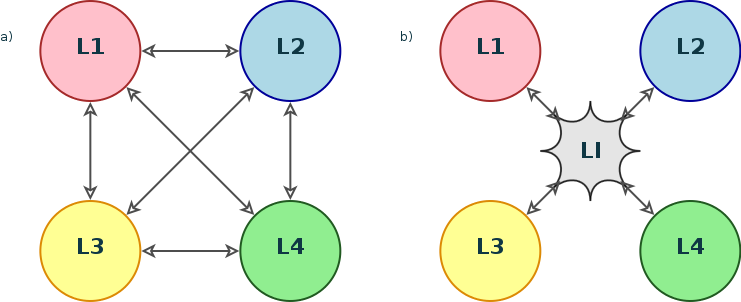
\includegraphics{interlingua.png}
\caption[Traducción directa y traducción con lengua intermedia.]{a) Grafo de traducciones necesarias en el caso de traducción directa
(se necesitan 12 diccionarios de traducción); b) Grafo de traducciones necesarias
utilizando una lengua puente (son necesarios únicamente 8 módulos de traducción).
Fuente: Wikimedia Commons.}\label{0.intro:fig-interlingua}\end{figure}

El mundo actual globalizado es un claro ejemplo de entorno multilingüe donde una
verdadera superación de la barrera del lenguaje solo puede acometerse utilizando una
interlingua. Un escenario de este tipo permitiría un acceso universal a la cultura y
una expansión comercial hacia nuevos mercados sin precedentes, los productos podrían
localizarse en la lengua nativa de cada cliente potencial sin incurrir en costes elevados.

Sin embargo, a pesar de estos beneficios, este tipo de traducción es una de las menos
utilizadas en la práctica, la mayoría son prototipos de investigación y solo el
proyecto KANT \footnote{
El proyecto Kant fue iniciado en 1989 por el Centro de Traducción Automática de
la Universidad Carnegie Mellon (Pittsburg) para la traducción de documentación
técnica. Más información puede ser consultada en su web:
\href{http://www.lti.cs.cmu.edu/Research/Kant/}{http://www.lti.cs.cmu.edu/Research/Kant/} (accedida 30 de marzo de 2015) y
también en Nyberg y Mitamura, 2000 (\phantomsection\label{0.intro:id31}{\hyperref[zreferences:nyberg2000]{\emph{{[}61{]}}}}).
} ha sido utilizado en un sistema comercial \phantomsection\label{0.intro:id27}{\hyperref[zreferences:brown2006]{\emph{{[}25{]}}}}, sin
embargo su aplicación se limita a la traducción de textos técnicos en inglés
controlado \footnote{
El adjetivo ``controlado'' aplicado a un lenguaje hace referencia a que el texto
original ha sido adaptado a una serie de reglas definidas de antemano con el
objetivo de mejorar su traducibilidad \phantomsection\label{0.intro:id33}{\hyperref[zreferences:schwitter2010]{\emph{{[}74{]}}}}.
} hacia francés, español y alemán \phantomsection\label{0.intro:id29}{\hyperref[zreferences:lonsdale1994]{\emph{{[}51{]}}}}.

Alansary \phantomsection\label{0.intro:id34}{\hyperref[zreferences:alansary2011]{\emph{{[}1{]}}}} identifica cinco características que debe cumplir una
interlingua:
\begin{itemize}
\item {} 
no puede ser ambigua,

\item {} 
debe ser capaz de representar todos los matices del texto,

\item {} 
tiene que ser universal para poder representar cualquier significado de cualquier
dominio,

\item {} 
debe representar únicamente el contenido independientemente de la representación
formal del lenguaje de origen, y

\item {} 
tiene que ser independiente tanto del lenguaje de origen como del de destino.

\end{itemize}

Teniendo en cuenta estas características ningún lenguaje natural puede ser utilizado
como interlingua puesto que no estará exento de ambigüedad e, igualmente, ninguna
interlingua puede diseñarse con la idea de ser utilizada por las personas ya que
con el tiempo evolucionará apartándose de la ortodoxia de estos principios.

En consecuencia, una lengua pívot para un sistema de traducción automática solo podrá ser
un lenguaje artificial. Este constructo, además de servir para realizar traducciones,
constituiría una herramienta de representación del conocimiento que podría ser utilizada
en cualquier aplicación de recuperación de información. Como tendremos ocasión de
exponer en el siguiente capítulo, el UNL constituye una propuesta muy interesante en este
sentido que ha contado con el apoyo de instituciones públicas de primer nivel y que
hoy en día se mantiene en desarrollo.


\section{La calidad de la traducción}
\label{0.intro:la-calidad-de-la-traduccion}
Uno de los apéndices del informe del ALPAC \phantomsection\label{0.intro:id35}{\hyperref[zreferences:pierce1966]{\emph{{[}64{]}}}} tuvo tanta
repercusión como el propio informe, se trata del apéndice 10 donde se describe
el experimento llevado a cabo por John B. Carroll para evaluar la calidad de las
traducciones, tanto humanas como automáticas. En su experimento se sometían
varias traducciones realizadas por humanos y por máquinas a la evaluación
de un conjunto de personas que las puntuaba según dos parámetros: inteligibilidad
y fidelidad.

El desarrollo de una medida que permita evaluar la calidad de una traducción es
un asunto de extremada importancia, generalmente el destinatario de la traducción o
el que la solicita no es capaz de comprender uno de los dos idiomas, por lo que
debe fiarse de que el contenido que está entregando o recibiendo se corresponde con
el texto original.

En el experimento de Carroll la evaluación era realizada por personas que daban una
puntuación a distintos fragmentos de los textos traducidos comparados con los
originales. En las conclusiones se muestra claramente cómo los textos producidos por
los sistemas automáticos obtienen valores muy por debajo de los realizados por
traductores.

En este documento abordamos precisamente este problema: la definición de una medida
de distancia entre el texto original y la traducción que permita valorar el
rendimiento de un sistema de traducción automática. Como tendremos la ocasión de
exponer en el próximo capítulo, nuestra medida se apoyará en la interlingua UNL para
poder realizar la comparación, tomará el grafo del texto original y medirá la
distancia al grafo resultante de convertir el texto traducido nuevamente a esta
interlingua (ver \hyperref[0.intro:fig-problema-interlingua]{figura  \ref*{0.intro:fig-problema-interlingua}}).
\begin{figure}[htbp]
\centering
\capstart

\includegraphics{graphviz-b4320435dfdacf521d0de69bb0728ea23c81445a.pdf}
\caption{Procedimiento de evaluación de una traducción con lengua intermedia.}\label{0.intro:fig-problema-interlingua}\end{figure}

El trabajo está organizado en siete capítulos. Tras esta introducción que permite
contextualizar la problemática relacionada con los sistemas de traducción, se realiza
una exposición en el capítulo 2 del estado del arte de los sistemas de traducción
basados en interlingua y los trabajos previos que sirven de soporte para el modelo
que propondremos. El capítulo 3 expone el problema que tratamos de abordar, el
capítulo 4 muestra las limitaciones y restricciones a las que nos vemos sometidos o
que tenemos que asumir a la hora de enfrentarnos a él. En el capítulo 5 se expone
el modelo desarrollado, que se somete a experimentación en el capítulo 6, donde también
se muestran los resultados de estas pruebas. Finalmente el capítulo 7 recoge las
conclusiones del trabajo, la valoración del autor sobre el mismo y las líneas
de investigación y desarrollo que deben continuarse para contribuir a la
resolución del problema propuesto.
\newpage

\chapter{Estado del Arte}
\label{1.state-of-the-art/index:estado-del-arte}\label{1.state-of-the-art/index::doc}
La base de los sistemas de traducción automáticos basados en una interlingua es
que esta debe representar todas las oraciones que tienen el mismo
significado de la misma manera, con el mismo conjunto de símbolos, independientemente
del idioma original del texto. Partiendo de esta representación única no ambigua
se generan las traducciones a todos los idiomas de destino como se muestra en
la \hyperref[1.state-of-the-art/index:fig-interlingua-esquema]{figura  \ref*{1.state-of-the-art/index:fig-interlingua-esquema}}.
\begin{figure}[htbp]
\centering
\capstart

\includegraphics{graphviz-d75f14de93610c0ebaaea65a76a65c56ba45b864.pdf}
\caption{Sistema de traducción automática basado en interlingua}\label{1.state-of-the-art/index:fig-interlingua-esquema}\end{figure}

Si convirtiéramos cualquiera de los textos traducidos de nuevo en la representación
en interlingua, deberíamos obtener una codificación idéntica a la que hemos
utilizado para generarlos \footnote{
Podrán existir diferencias debidas a fenómenos lingüísticos como la paráfrasis y
también pérdidas de significado debidas a limitaciones de la lengua de destino si esta
no es capaz de representar toda la riqueza semántica del texto original.
}. La calidad de la traducción en cuanto a su fiabilidad,
entendida como contenido semántico transmitido, estará por lo tanto directamente
relacionada con la proximidad entre las dos representaciones en interlingua; así
una medida adecuada de distancia o de similaridad entre ambas representaciones resulta
ser una herramienta de extremada utilidad para evaluar un sistema de traducción automática.

En este capítulo estudiamos el estado del arte de los sistemas de representación del
conocimiento que son utilizados como interlinguas, y en concreto nos centraremos en
aquellos cuya representación formal es un grafo; posteriormente expondremos las
medidas que se han propuesto en la bibliografía para estudiar la similaridad entre dos
grafos, veremos cómo evaluar la distancia semántica entre conceptos y textos, y
finalmente repasaremos los modelos propuestos que integran lo anterior para evaluar
la distancia entre grafos conceptuales (manifiestan una distancia debida a la estructura
del grafo y también al contenido de los nodos) analizando en profundidad cuáles son sus
principales aportaciones y las dificultades que aún están presentes.


\section{Sistemas de representación del conocimiento}
\label{1.state-of-the-art/i.representacion-conocimiento::doc}\label{1.state-of-the-art/i.representacion-conocimiento:sistemas-de-representacion-del-conocimiento}
Las máquinas no pueden trabajar con un lenguaje plagado de ambigüedades y de contextos
culturales subyacentes, necesitan de una representación formal explícita del
discurso para poder entenderlo y trabajar con él, así pues debemos ser capaces de
codificar nuestras ideas en una estructura rígida, estructurar la actividad
cognitiva humana en un sistema de representación inteligible por los algoritmos y
modelos programados.

Pensamiento y Lenguaje están indisolublemente unidos, las estructuras conceptuales,
si bien son diferentes de las estructuras lingüísticas, mantienen con estas una
estrecha relación: para conocerlas, identificarlas y distinguirlas precisamos del
lenguaje natural, pero también para describirlas y representarlas. Sin embargo, el
aspecto lingüístico no es constitutivo de esas estructuras por más que sea su
mediador (Izquierdo Arroyo, 1995 \phantomsection\label{1.state-of-the-art/i.representacion-conocimiento:id1}{\hyperref[zreferences:izquierdoarroyo1995]{\emph{{[}41{]}}}}).

La bibliografía contemporánea recoge la problemática de las estructuras conceptuales
desde que en 1966 apareciera el libro de Shera sobre la ``Documentación y la Organización
del Conocimiento'' \phantomsection\label{1.state-of-the-art/i.representacion-conocimiento:id2}{\hyperref[zreferences:shera1966]{\emph{{[}79{]}}}}; se trata de un problema que compete a las llamadas
Ciencias Cognitivas las cuales engloban disciplinas muy diferentes: la dimensión individual es
objeto de la Psicología, pero también hay una dimensión social que será objeto de la Sociología
y que se basa en el ``principio de cooperación'' \phantomsection\label{1.state-of-the-art/i.representacion-conocimiento:id3}{\hyperref[zreferences:grice1975]{\emph{{[}32{]}}}} que establece que el discurso
es una actividad colaborativa que se rige por unas máximas aceptadas tácitamente por todos
cuantos participan en la conversación.


\subsection{Teoría de la Dependencia Conceptual}
\label{1.state-of-the-art/i.representacion-conocimiento:teoria-de-la-dependencia-conceptual}\label{1.state-of-the-art/i.representacion-conocimiento:teoria-dependencia-conceptual}
La principal dificultad para desarrollar los sistemas de comprensión del discurso por
ordenador radica en proporcionarles esquemas conceptuales y conocimientos sobre el
mundo que les permita realizar inferencias. Uno de los primeros esfuerzos en este sentido
lo encontramos en 1979 en la obra de Roger C. Schank y Robert P. Abelson \phantomsection\label{1.state-of-the-art/i.representacion-conocimiento:id4}{\hyperref[zreferences:schank1977]{\emph{{[}73{]}}}}
donde se proponen dar con un ``aparato general para un intento de representar todo o cualquier
conocimiento'', estudiando ``cómo funciona la comprensión humana'' puesto que ``si entendemos
cómo comprende el ser humano, podremos saber cómo conseguir que un ordenador entienda,
y viceversa''. Esta doctrina se apoya en la Teoría de la Dependencia Conceptual
\phantomsection\label{1.state-of-the-art/i.representacion-conocimiento:id5}{\hyperref[zreferences:schank1969]{\emph{{[}72{]}}}} que es ``una teoría de la representación del significado de las frases'',
cuyo axioma principal consiste en que ``para cualesquiera dos frases que son idénticas en
significado, sin tener en cuenta las diferencias en el lenguaje, existe una única
representación'' \footnote{
Las citas textuales, traducciones del original, han sido tomadas
de \phantomsection\label{1.state-of-the-art/i.representacion-conocimiento:id8}{\hyperref[zreferences:izquierdoarroyo1995]{\emph{{[}41{]}}}}.
}, en esta unicidad que supone una correspondencia biunívoca entre
significado y representación nos fundamentamos para afirmar que es posible hablar de
distancia semántica como herramienta para caracterizar los sistemas de traducción
automática.

Schank y Abelson estructuran el conocimiento en una secuencia de eventos,
guiones o \emph{scripts} que representan a través de lo que llaman \emph{primitivos léxicos}, los cuales
pueden hacer referencia tanto a una acción (con la forma Actor-Acción-Objeto-Dirección
{[}-Instrumento{]}) como a un estado (Objeto-(está en)-Estado{[}-con Valor{]}). Los autores
identifican 11 actos primitivos que son los constituyentes esenciales de cualquier acción
más compleja, con lo que las reglas de inferencia y razonamiento deben definirse sobre
un conjunto finito y reducido de elementos. A partir de los guiones almacenados en la
memoria, el ser humano y el ordenador pueden elaborar razonamientos y responder a las
consultas o peticiones de información.


\subsection{Grafos conceptuales}
\label{1.state-of-the-art/i.representacion-conocimiento:grafos-conceptuales}\label{1.state-of-the-art/i.representacion-conocimiento:id9}
La característica fundamental que debe tener una interlingua es su capacidad para
representar cualquier tipo de conocimiento de una forma no ambigua. Una de las
herramientas más potentes para la representación del conocimiento que además
permite realizar inferencias son los grafos conceptuales (CG, \emph{Conceptual Graph}),
éstos son introducidos por Sowa en 1976 \phantomsection\label{1.state-of-the-art/i.representacion-conocimiento:id10}{\hyperref[zreferences:sowa1976]{\emph{{[}82{]}}}} donde los define como:
\begin{quote}

A \emph{conceptual graph} is a finite, connected, undirected, bipartite graph with
nodes of one type called \emph{concepts} and nodes of the other type called
\emph{conceptual relations}. A conceptual graph may consist of a single concept,
but it cannot have conceptual relations with unattached links. \footnote{
Traducción: Un \emph{grafo conceptual} es un grafo bipartito finito, conectado y no
dirigido en el que los nodos de un tipo se llaman \emph{conceptos} y los del otro tipo se
conocen como \emph{relaciones conceptuales}. Un grafo conceptual puede constar de un único
concepto, pero no puede contener relaciones conceptuales que tengan enlaces sin conectar.
}
(Cursivas en el original)
\end{quote}

La primera aproximación de Sowa a los grafos conceptuales la realiza en el contexto
de las bases de datos y los sistemas de recuperación de información \footnote{
John F. Sowa desarrolla los CGs en más profundidad en sus libros
\emph{Conceptual Structures: Information Processing in Mind and Machine}, Addison Wesley
Publishing Co., London, UK, 1984 y \emph{Knowledge Representation: Logical, Philosophical and
Computational Foundations}, Brooks Cole Publishing Co., Pacific Grove, CA, 2000.
}, como una herramienta
intermedia de comunicación entre los usuarios y las máquinas: el grafo describe el
significado desde el punto de vista del humano, pero su codificación puede ser fácilmente
interpretada por un programa:
\begin{itemize}
\item {} 
Los \textbf{conceptos} están representados por cajas que contienen un etiqueta identificativa
del elemento cognitivo que representan, que puede tratarse de cualquier entidad real o
abstracción. Sowa, además, introduce una propiedad de ordenamiento entre los conceptos
que le permite crear una estructura jerárquica; esta propiedad, representada por \(<\),
puede aplicarse a dos conceptos cualesquiera \(a\) y \(b\), de tal forma que
si se cumple \(a < b\) entonces \(a\) es un \emph{subtipo} de \(b\), es decir,
representa un concepto más específico. No hay ninguna restricción que impida que un
concepto sea \emph{subtipo común} de varios otros, por lo que la jerarquía que puede
construirse de este modo será un grafo acíclico dirigido (DAG, \emph{Directed Acyclic Graph}).

\item {} 
Las \textbf{relaciones conceptuales} están representadas por círculos en el grafo y pueden tener una
o más conexiones. Estas relaciones actúan como restricciones al seleccionar qué conceptos
pueden unir \phantomsection\label{1.state-of-the-art/i.representacion-conocimiento:id14}{\hyperref[zreferences:clancey1985]{\emph{{[}17{]}}}}, de esta forma incorporan una dimensión lógica en los grafos.

\item {} 
En Sowa (2003) \phantomsection\label{1.state-of-the-art/i.representacion-conocimiento:id15}{\hyperref[zreferences:sowa2003]{\emph{{[}83{]}}}} el autor introduce los \emph{nested graph models} (NGM) que
permiten expresar el \textbf{contexto} de una relación, así es posible incorporar lógica modal y
temporal.

\end{itemize}

Sowa habla de ontologías en relación a los nodos-concepto, indica que la selección de las
categorías ontológicas debe ser el primer paso para diseñar una base de datos, de
conocimiento o un sistema orientado a objetos \phantomsection\label{1.state-of-the-art/i.representacion-conocimiento:id17}{\hyperref[zreferences:shapiro2012]{\emph{{[}78{]}}}}; sin embargo no
introduce ningún tipo de restricción en cuanto a los tipos de relaciones existentes que
pueden aparecer en el grafo.
\begin{figure}[htbp]
\centering
\capstart

\scalebox{0.800000}{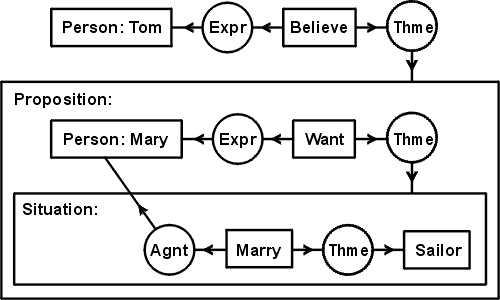
\includegraphics{sowagraph.png}}
\caption[Ejemplo de grafo conceptual con contextos.]{Un grafo conceptual con dos contextos anidados. El grafo representa la oración \emph{Tom believes that Mary wants to marry a sailor}. Imagen extraída de Sowa (2003) \phantomsection\label{1.state-of-the-art/i.representacion-conocimiento:id18}{\hyperref[zreferences:sowa2003]{\emph{{[}83{]}}}}.}\label{1.state-of-the-art/i.representacion-conocimiento:fig-sowa}\end{figure}


\subsection{Semántica estructural}
\label{1.state-of-the-art/i.representacion-conocimiento:semantica-estructural}
En los nodos de tipo \emph{concepto} de los CGs tiene que tener cabida cualquier entidad real
o abstracta y esta tiene que poder expresarse de una manera no ambigua. En su artículo de
1976 \phantomsection\label{1.state-of-the-art/i.representacion-conocimiento:id19}{\hyperref[zreferences:sowa1976]{\emph{{[}82{]}}}} Sowa ya indica que estos conceptos son meros identificadores y que
por conveniencia son representados con una breve etiqueta en inglés, pero podría tratarse
de un número o una dirección de memoria en un ordenador.

Más importante es la jerarquización entre conceptos que introduce a través de la propiedad
\(<\) a la que hemos hecho mención, en artículos posteriores Sowa empezará a hablar de
ontología y de categorías al hacer referencia a la jerarquía de conceptos.

El término \emph{ontología} hace referencia a una parte de la metafísica que trata del ser en
general y sus propiedades trascendentales; es un concepto que se ha estudiado desde la época
clásica con la intención de realizar una clasificación de todo lo que \emph{es}.
Sin embargo, nos interesa más abordar las ontologías desde el punto de vista de la
Ingeniería del Conocimiento, en este ámbito
una de las definiciones más extendidas y aceptadas es la que se ofrece en \phantomsection\label{1.state-of-the-art/i.representacion-conocimiento:id20}{\hyperref[zreferences:studer1998]{\emph{{[}84{]}}}}:
\emph{``An ontology is a formal, explicit specification of a shared conceptualization''} \footnote{
Traducción: una ontología es una especificación explícita y formal de un
conceptualización compartida.
}. Por
\emph{conceptualización} se entiende una modelización abstracta de un fenómeno identificando sus
conceptos relevantes. Por \emph{explícito} se hace referencia a que tanto los conceptos como sus
relaciones y restricciones tienen que estar definidas explícitamente. Al ser \emph{formal} la
ontología puede procesarse mediante un programa informático (no estará expresada en lenguaje
natural). Y también tiene que ser \emph{compartida}, tiene que recoger un conocimiento consensuado,
ha de ser aceptada por un grupo.

En los sistemas de traducción automática una ontología de los conceptos deberá recoger toda
la realidad expresable en cualquier lenguaje natural, todos los significados posibles a los
que haga referencia cualquier significante, ya sean realidades o pensamientos, abstracciones
o acciones.

El estudio de los conceptos, los referentes, los símbolos, etc. es una rama de la lingüística que
se desarrolla como ciencia durante el siglo XX y de forma sistemática a partir de los 1960s.
La semiótica comienza su andadura con lingüísticas y filólogos como Ferdinand de Saussure,
Louis Hjelmslev, Roman Jakobson y Ludwig Wittgenstein en Europa y paralelamente en
Estados Unidos con Charles Sanders Peirce. Peirce y Saussure son contemporáneos y abordan el
mismo problema, la creación de una \emph{ciencia de los signos}, pero desde perspectivas diferentes.
Saussure, lingüista, la aborda desde una perspectiva psicosocial e indica que se trata de una
nueva ciencia a la que llama \emph{semiología}, Peirce considera que esta
ciencia de los signos ya existe desde la antigüedad, aunque no plenamente desarrollada
\phantomsection\label{1.state-of-the-art/i.representacion-conocimiento:id23}{\hyperref[zreferences:castanares2000]{\emph{{[}15{]}}}}, así su trabajo consistió en la exploración, sistematización y ampliación
de la lógica heredada de Aristóteles \phantomsection\label{1.state-of-the-art/i.representacion-conocimiento:id24}{\hyperref[zreferences:peirce1902]{\emph{{[}7{]}}}}. Peirce desarrolló los grafos
existenciales, que son el punto de partida para los grafos conceptuales de John F. Sowa.

Fruto de estos estudios en el campo de la lingüística se realizan avances muy importantes
relacionados con el significado de las palabras, nos interesa aquí hacer referencia a la
semántica estructural y las principales relaciones que se dan entre significados y que
han de ser considerados en una ontología de conceptos \phantomsection\label{1.state-of-the-art/i.representacion-conocimiento:id25}{\hyperref[zreferences:wpsemantica]{\emph{{[}99{]}}}}:
\begin{itemize}
\item {} 
\textbf{Hiperonimia}: es la relación que se da entre una palabra (hiperónimo) cuyo significado
está totalmente incluido en los significados de otras más específicas (hipónimos).

\item {} 
\textbf{Hiponimia}: es la relación en la que el significado de una palabra más específica
(hipónimo) contiene todos los rasgos de significado del término más general (hiperónimo).
Dos hipónimos de un mismo hiperónimo, son cohipónimos.

\item {} 
\textbf{Holonimia}: es la relación que se establece entre una palabra (holónimo) y otra u
otras (merónimos) que designan partes de lo denotado por la primera. No se trata de una
relación entre significados, sino de rasgos extralingüísticos.

\item {} 
\textbf{Meronimia}: un merónimo designa una parte de la realidad nombrada por un holónimo.

\end{itemize}

Atendiendo a las propias palabras en relación con sus significados encontramos los siguientes
fenómenos \phantomsection\label{1.state-of-the-art/i.representacion-conocimiento:id26}{\hyperref[zreferences:wpsemantica]{\emph{{[}99{]}}}}:
\begin{itemize}
\item {} 
\textbf{Monosemia}: palabras que tienen un único significado o acepción.

\item {} 
\textbf{Polisemia}: una sóla palabra tiene varios significados, estando todos ellos emparentados
semánticamente.

\item {} 
\textbf{Homonimia}: varios significados asociados a una misma forma, pero con orígenes diferentes.

\item {} 
\textbf{Sinonimia}: es la relación entre dos términos de significados similares e intercambiables
en el discurso por pertenecer a la misma categoría sintáctica.

\item {} 
\textbf{Antonimia}: es la relación que mantienen dos palabras cuyos significados se oponen.

\end{itemize}

En la \hyperref[1.state-of-the-art/i.representacion-conocimiento:fig-wordnet-lightning]{figura  \ref*{1.state-of-the-art/i.representacion-conocimiento:fig-wordnet-lightning}} se muestran algunos casos de hiperonimia/hiponimia y
holonimia/meronimia en torno a la palabra \emph{candle}. En la misma imagen se puede ver también el
fenómeno polisémico de esta palabra en inglés que puede denotar los conceptos de \emph{vela}, \emph{candela}
o hacer referencia al verbo, inexistente en español, para referirse a la realización de una
ovoscopia.
\begin{figure}[htbp]
\centering
\capstart

\includegraphics{graphviz-cc85bd4f4e8f23b4dace53125aef3808c14b8c04.pdf}
\caption[Estructura de relaciones semánticas de WordNet en torno a la palabra *candle*.]{Esquema de relaciones semánticas en torno a la palabra \emph{candle}, que en inglés hace referencia a los conceptos \emph{vela} y \emph{candela}, y también al verbo utilizado para la realización de una \emph{ovoscopia}. Cada nodo representa un concepto (representado por varias palabras sinónimas). Las relaciones han sido extraídas de Wordnet v3.1.}\label{1.state-of-the-art/i.representacion-conocimiento:fig-wordnet-lightning}\end{figure}


\subsection{WordNet}
\label{1.state-of-the-art/i.representacion-conocimiento:id27}\label{1.state-of-the-art/i.representacion-conocimiento:wordnet}
Una de los esfuerzos más importantes para realizar una ontología de conceptos es WordNet
\phantomsection\label{1.state-of-the-art/i.representacion-conocimiento:id28}{\hyperref[zreferences:miller1990]{\emph{{[}55{]}}}} \phantomsection\label{1.state-of-the-art/i.representacion-conocimiento:id29}{\hyperref[zreferences:fellbaum1998]{\emph{{[}28{]}}}}, se trata de una red de conceptos que contiene
información codificada manualmente sobre sustantivos, verbos, adjetivos y adverbios
en inglés; los términos que representan un mismo concepto están agrupados en \emph{synsets} y
son estos elementos los que constituyen los nodos de la red.
WordNet se creó en el Laboratorio de Ciencia Cognitiva de la Universidad de Princeton en
1985 bajo la dirección del profesor de psicología George Armitage Miller (1920-2012).

Un \emph{synset} es un conjunto de palabras de la misma categoría gramatical que hacen
referencia a la misma realidad extralingüística y por lo tanto pueden ser intercambiadas
en un texto sin afectar al significado. Son elementos semánticamente equivalentes.
Las palabras polisémicas aparecerán múltiples veces en \emph{synset} diferentes.
WordNet se encuentra actualmente en su versión 3.1 y se puede acceder online en
\code{https://wordnet.princeton.edu}, cuenta con más de 117.000 synsets.

Las principales relaciones codificadas en WordNet son las de hiperonimia/hiponimia, seguidas
por las de holonimia/meronimia, ambas estructuran los conceptos en jerarquías como la que
se muestra en la \hyperref[1.state-of-the-art/i.representacion-conocimiento:fig-wordnet-lightning]{figura  \ref*{1.state-of-the-art/i.representacion-conocimiento:fig-wordnet-lightning}}. Los verbos también están organizados
en jerarquías arbóreas donde los hijos expresan maneras cada vez más específicas de realizar
la acción (troponimia). Los adjetivos incluyen relaciones de antonimia, similaridad
semántica y también relaciones con los sustantivos de los cuales derivan. En cuanto a los
adverbios, son la categoría gramatical menos representada, en general están relacionados
con los adjetivos de los que derivan.

WordNet es un recurso valiosísimo para cualquier tipo de aplicación con contenido semántico,
como lo es una interlingua para representación del conocimiento; así WordNet se puede utilizar
como un diccionario para identificar sin ambigüedades los conceptos que se utilizan en los
nodos de un grafo conceptual y también, como veremos posteriormente, es una herramienta ideal
para medir distancias semánticas entre conceptos.


\subsection{EuroWordNet}
\label{1.state-of-the-art/i.representacion-conocimiento:eurowordnet}
La importancia probada de WordNet en la investigación asociada a lingüística computacional
condujo a la creación de un proyecto europeo (LE-2 4003 y LE-4 8328) para generar \emph{wordnets}
en otros idiomas europeos y unir todos ellos en una base de datos multilingüe que permite,
a partir de una palabra, consultar palabras similares en cualquier otro idioma \footnote{
EuroWordNet: Building a multilingual database with wordnets for several European
languages. \href{http://www.illc.uva.nl/EuroWordNet/}{http://www.illc.uva.nl/EuroWordNet/} (accedida en mayo de 2015)
}.

Los primeros cuatro idiomas que se adhirieron al proyecto fueron holandés (Universidad de
Amsterdam), italiano (CNR, Pisa), español (Fundación Universidad Empresa) e inglés (Universidad
de Sheffield, adaptando el WordNet original); posteriormente se incorporan el checo, estonio,
alemán y francés \phantomsection\label{1.state-of-the-art/i.representacion-conocimiento:id32}{\hyperref[zreferences:vossen1998]{\emph{{[}95{]}}}}.

La principal contribución de este proyecto es la multilingualidad, el \emph{wordnet} de cada idioma
es específico, pero todos ellos se integran en una base de datos única a través de un índice
interlingual (ILI, \emph{inter-lingual index}) que conecta los \emph{synsets} que son equivalentes
en los diferentes idiomas.

El proyecto se dió por finalizado en 1999 con la definición de la base de datos, las relaciones,
la \emph{Top Concept Ontology} (una ontología con 63 conceptos abstractos que se utilizaría para
clasificar al resto de conceptos más concretos) y la definición del índice ILI. Con
posterioridad se han seguido desarrollando los \emph{wordnets} de cada idioma y se han sumado
idiomas nuevos que han utilizado las especificaciones del EuroWordNet para generar sus bases
de datos.

Actualmente el testigo ha sido recogido por la \emph{Global WordNet Association} \footnote{
The Global WordNet Association. \href{http://globalwordnet.org/}{http://globalwordnet.org/} (accedido en mayo de 2015).
} que intenta
promover el desarrollo, difusión y estandarización de los \emph{wordnets} que se vayan realizando.

Apoyándose en estas redes de conceptos se han desarrollado multitud de aplicaciones
de procesamiento de lenguaje natural, y recursos lingüísticos como el proyecto \emph{MEANING
Multilingual Central Repository} \phantomsection\label{1.state-of-the-art/i.representacion-conocimiento:id35}{\hyperref[zreferences:atserias2004]{\emph{{[}5{]}}}}, ontologías como SUMO \phantomsection\label{1.state-of-the-art/i.representacion-conocimiento:id36}{\hyperref[zreferences:niles2001]{\emph{{[}60{]}}}}
o la \emph{EuroWordNet Top Concept Ontology} que ya hemos citado \phantomsection\label{1.state-of-the-art/i.representacion-conocimiento:id37}{\hyperref[zreferences:alvez2008]{\emph{{[}2{]}}}}.


\subsection{Interlingua}
\label{1.state-of-the-art/i.representacion-conocimiento:interlingua}
En el capítulo introductorio hablamos de la traducción automática utilizando sistemas basados
en interlinguas (ver \DUspan{xref,std,std-ref}{sección 1.3}) como la aproximación
adecuada en un entorno multilingüe, sin embargo existen algunos problemas que dificultan
su utilización.

El argumento más relevante en contra del uso de las interlinguas está relacionado con el nivel
de abstracción y universalidad que debe tener esta lengua, lo que la convertiría en inviable
económicamente \phantomsection\label{1.state-of-the-art/i.representacion-conocimiento:id38}{\hyperref[zreferences:martins2002]{\emph{{[}87{]}}}}: no solo debería ser capaz de expresar cualquier significado
de cualquier lengua sino que también tendría que poder trabajar con las particularidades
cognitivas de todas las culturas, un problema sin acotar. Por ejemplo, una interlingua de
carácter universal debería ser capaz de representar la lógica trivalente del
aymara \phantomsection\label{1.state-of-the-art/i.representacion-conocimiento:id39}{\hyperref[zreferences:rojas1985]{\emph{{[}33{]}}}}, que supone un desafío para el mundo occidental heredero de la
lógica dicotómica aristotélica.
Hutchins \phantomsection\label{1.state-of-the-art/i.representacion-conocimiento:id40}{\hyperref[zreferences:hutchins1992]{\emph{{[}38{]}}}} expone otros muchos problemas acompañados de una gran
colección de ejemplos.


\subsubsection{Eurotra}
\label{1.state-of-the-art/i.representacion-conocimiento:eurotra}
Ante la dificultad (en la práctica insalvable) que supone construir una interlingua universal,
se proponen interlinguas restringidas que permitan una representación exacta para un
conjunto cerrado de lenguas.
Un ejemplo de este tipo ha sido el proyecto Eurotra que se concibe en 1978 y se dota de fondos
en noviembre de 1982 con el objetivo de producir traducciones
satisfactorias para todos los idiomas de la Comunidad Europea \phantomsection\label{1.state-of-the-art/i.representacion-conocimiento:id41}{\hyperref[zreferences:hutchins1992a]{\emph{{[}39{]}}}}.
Es un proyecto a medio camino entre una interlingua y los
sistemas \emph{transfer} entre pares de lenguas.

El proyecto se detiene en 1992 sin que lograra desembocar en un sistema comercial de traducción
automática, sin embargo sí que llegó a crear un prototipo de investigación y sentó las
bases para el nacimiento de grupos de investigación asociados con la traducción en los
países del sur del continente europeo.


\subsubsection{PIVOT}
\label{1.state-of-the-art/i.representacion-conocimiento:pivot}
A finales de los 1980s también se iniciaba el proyecto de traducción automática multilingüe
conocido como PIVOT; a diferencia del programa EUROTRA, este sí planteaba la creación de una
interlingua que sirviera como eje de las traducciones.
No era el único proyecto en este sentido, Fujitsu lo estaba haciendo en su proyecto ATLAS
(Dr. Uchida) y la universidad Carnegie Mellon de Pittsburg (USA) con KANT (Jaime Carbonell).

PIVOT estaba dirigido por el Dr. Muraki desde Japón y patrocinado por NEC. En España, la
Universidad Politécnica de Madrid se encargó de desarrollar el módulo de español cuyo
objetivo era convertir los textos de español en la interlingua y generar las traducciones
a español.

Este proyecto también finaliza en 1992, al igual que EUROTRA. El proyecto ATLAS, por su
parte, aún puede ser encontrado en la página web de Fujitsu como un producto comercial
relacionado con la traducción, aunque solo entre el par de lenguas inglés-japonés \footnote{
Fujitsu. ATLAS V14. Información disponible en \href{https://www.fujitsu.com/global/products/software/packaged-software/translation/atlas/}{https://www.fujitsu.com/global/products/software/packaged-software/translation/atlas/} (accedido en junio de 2015)
}.


\subsection{El lenguaje universal UNL}
\label{1.state-of-the-art/i.representacion-conocimiento:el-lenguaje-universal-unl}
Un paso adelante en las interlinguas para representación del conocimiento es el lenguaje
universal (UNL, \emph{Universal Networking Language}). Este \emph{lenguaje} surgió como una
iniciativa del Instituto de Estudios Avanzados de la Universidad de la Naciones Unidas
en 1996 con el objetivo de eliminar las barreras lingüísticas para el comercio y la
educación.

La representación de un texto en UNL se realiza oración por oración, cada oración se
codifica en un hipergrafo donde los conceptos son los nodos y las relaciones entre ellos
constituyen los arcos. Este hipergrafo también puede ser representado como un conjunto
de relaciones binarias que enlazan los conceptos presentes en la oración.

Los conceptos se representan con etiquetas literales que reciben el nombre de
\emph{palabras universales} (UW, \emph{Universal Words}) que además pueden ir acompañadas de
varios atributos (se utiliza el símbolo \code{@} para indicarlos) que
permiten mostrar más informacón sobre el uso específico del concepto en la oración
original \phantomsection\label{1.state-of-the-art/i.representacion-conocimiento:id44}{\hyperref[zreferences:uchida1999]{\emph{{[}93{]}}}}. Estas UWs son el equivalente a los nodos-concepto de Sowa
y a los \emph{synsets} de WordNet.

Como ejemplo, mostramos el utilizado por Uchida y Zhu en \phantomsection\label{1.state-of-the-art/i.representacion-conocimiento:id45}{\hyperref[zreferences:uchida2001]{\emph{{[}91{]}}}} donde muestran
la codificación de la oración ``Hace tiempo, en la ciudad de Babilonia, la gente comenzó a
construir una torre enorme, que parecía alcanzar los cielos.'' tanto en su forma
gráfica (\hyperref[1.state-of-the-art/i.representacion-conocimiento:fig-example-unl]{figura  \ref*{1.state-of-the-art/i.representacion-conocimiento:fig-example-unl}}) como codificada (\hyperref[1.state-of-the-art/i.representacion-conocimiento:code-example-unl]{listado  \ref*{1.state-of-the-art/i.representacion-conocimiento:code-example-unl}}).
\begin{figure}[htbp]
\centering
\capstart

\includegraphics{graphviz-bd0cbd4fd50b08c30514ed96807eb2e28ed03eae.pdf}
\caption[Ejemplo de representación gráfica de una oración codificada en UNL.]{Representación gráfica en UNL de la oración ``Hace tiempo, en la ciudad de Babilonia, la gente comenzó a construir una torre enorme, que parecía alcanzar los cielos.''. El atributo \code{@entry} indica el concepto principal de la oración.}\label{1.state-of-the-art/i.representacion-conocimiento:fig-example-unl}\end{figure}

En el ejemplo indicado aparecen numerosas relaciones como \code{mod}, \code{agt}, \code{aoj}, etc.
que indican la relación entre los conceptos (UWs) que enlazan, aparecen varias UWs como
\code{city(icl\textgreater{}region)}, \code{tower(icl\textgreater{}building)} que indican objetos o \code{seem(icl\textgreater{}be)},
\code{begin(icl\textgreater{}do)} que son verbos, e incluso adjetivos como \code{huge(icl\textgreater{}big)} o el adverbio
\code{long ago(icl\textgreater{}ago)}; también aparece una UW que es un nombre propio de ciudad
\code{Babylon(iof\textgreater{}city)}. Muchas UWs están acompañadas por varios attributos como \code{@past},
\code{@def} o \code{@entry}.
Las palabras universales UWs y las relaciones están diseñadas para representar el contenido
objetivo del texto (el mensaje, la información, el contenido semántico), mientras que los
atributos codifican rasgos gramaticales del lenguaje, intencionalidad, etc. que pueden
no ser representables en todas las lenguas.

La principal diferencia entre el UNL y otros sistemas de representación del conocimiento como
los grafos conceptuales (ver \hyperref[1.state-of-the-art/i.representacion-conocimiento:grafos-conceptuales]{sección  \ref*{1.state-of-the-art/i.representacion-conocimiento:grafos-conceptuales}}) o el \emph{Resource Description
Framework} (RDF) \phantomsection\label{1.state-of-the-art/i.representacion-conocimiento:id46}{\hyperref[zreferences:brickley2014]{\emph{{[}8{]}}}} es que el número y el significado de las relaciones y
atributos deben formar parte del estándar \phantomsection\label{1.state-of-the-art/i.representacion-conocimiento:id47}{\hyperref[zreferences:teixeiramartins2005]{\emph{{[}86{]}}}}.

Antes de continuar con la exposición del lenguaje UNL debe hacerse notar que actualmente todo
el consorcio UNL no comparte las mismas especificaciones y los grupos originales de trabajo
están divergiendo en sus líneas de investigación y estándares. La Comunidad Europea ha dejado
de financiar el proyecto y no ha vuelto a mostrar interés por él \phantomsection\label{1.state-of-the-art/i.representacion-conocimiento:id48}{\hyperref[zreferences:tovar2000]{\emph{{[}88{]}}}} y es la
Fundación UNDL quien se encarga de coordinar los diferentes Centros de Lengua siendo éstos
ahora los que tienen que buscar financiación para mantener la iniciativa.

Asimismo la inactividad de la Fundación UNDL desembocó en la creación del
Consorcio UNL \footnote{
El acuerdo de constitución del Consorcio UNL puede ser consultado en \href{http://www.unl.fi.upm.es/consorcio/archivos/term\_constitution.pdf}{http://www.unl.fi.upm.es/consorcio/archivos/term\_constitution.pdf} (accedido en junio de 2015).
} en 2005 en el marco de la conferencia CICLING (Méjico); en 2006 este
consorcio adoptó el nombre Consorcio U++ \footnote{
Datos históricos extraídos de la web del Consorcio U++. \href{http://www.unl.fi.upm.es/consorcio/index.php}{http://www.unl.fi.upm.es/consorcio/index.php} (accedido en junio de 2015).
}.

La última especificación del lenguaje realizada por la UNDL Fundation (aunque no es aceptada
por parte del Consorcio U++) es la Version II (16 de febrero de 2014) \phantomsection\label{1.state-of-the-art/i.representacion-conocimiento:id53}{\hyperref[zreferences:zhu2014]{\emph{{[}102{]}}}} que
incluye 57 relaciones y 94 atributos.
Las UWs no son un conjunto cerrado, cualquier persona puede proponer nuevas UWs que expresen
un concepto no contemplado hasta el momento, aunque en teoría existe \footnote{
A pesar de que se habla de la \emph{UNL Knowledge Base} o más recientemente Ontología UNL en
varios entradas bibliográficas, el autor no ha sido capaz de encontrar esta base de datos ni
de obtener una referencia cierta a la misma.
} una base de datos,
\emph{UNL Knowledge Base} u Ontología UNL, con todas las UWs aceptadas y sus
relaciones \phantomsection\label{1.state-of-the-art/i.representacion-conocimiento:id55}{\hyperref[zreferences:zhu2002]{\emph{{[}92{]}}}}.


\subsubsection{Palabras universales (UWs)}
\label{1.state-of-the-art/i.representacion-conocimiento:palabras-universales-uws}
Las UWs constituyen una red de palabras similar a la vista en WordNet (\hyperref[1.state-of-the-art/i.representacion-conocimiento:wordnet]{sección  \ref*{1.state-of-the-art/i.representacion-conocimiento:wordnet}}),
UNL tiene las mismas cuatro categorías de conceptos: sustantivos, verbos, adjetivos y adverbios.
Las UWs se forman utilizando una palabra inglesa como etiqueta seguida de un conjunto de
restricciones:
\begin{gather}
\begin{split}<UW> ::= <headword> [<constraint \quad list>]\end{split}\notag
\end{gather}
donde cada una de las partes es:
\begin{itemize}
\item {} 
La \emph{headword} es una expresión en inglés (usualmente es una palabra, pero puede ser una
palabra compuesta o una oración si es necesario) que representa un conjunto de términos
a los que hace referencia esa expresión en inglés, se conoce como \emph{Basic UW}. Si no
existe una etiqueta en inglés para hacer referencia al concepto, entonces se utiliza la
palabra correspondiente en otro idioma y la UW se conoce como \emph{Extra UW}.

\item {} 
La lista de restricciones sirve para desambiguar los distintos significados a los que puede
hacer referencia una misma \emph{headword}. Cada restricción está formada por una relación UNL
y otra UW previamente definida que se combina con esta UW en dicha relación. Estas UWs
desambiguadas se conocen como \emph{Restricted UW}.

\end{itemize}

La \hyperref[1.state-of-the-art/i.representacion-conocimiento:table-uws-example]{tabla  \ref*{1.state-of-the-art/i.representacion-conocimiento:table-uws-example}} muestra algunos ejemplos de UWs con los significados
correspondientes; aparecen algunas UWs básicas como \emph{go} o \emph{house}, UWs restringidas y
también ejemplos de UWs extra.


\begin{threeparttable}
\capstart\caption{Ejemplos de palabras universales (UWs).}
\label{1.state-of-the-art/i.representacion-conocimiento:table-uws-example}
\begin{tabulary}{\linewidth}{|p{0.2\linewidth}|p{0.2\linewidth}|p{0.2\linewidth}|p{0.25\linewidth}|}
\hline
\textsf{\relax 
\textbf{UW}
} & \textsf{\relax 
\textbf{Headword}
} & \textsf{\relax 
\textbf{Restricciones}
} & \textsf{\relax 
\textbf{Significado}
}\\
\hline
go
 & 
go
 &  & 
Ir
\\
\hline
house
 & 
house
 &  & 
Casa
\\
\hline
state(icl\textgreater{}country)
 & 
state
 & 
icl\textgreater{}country
 & 
País
\\
\hline
state(icl\textgreater{}region)
 & 
state
 & 
icl\textgreater{}region
 & 
Región de un país
\\
\hline
state( icl\textgreater{}express( agt\textgreater{}thing, gol\textgreater{}person, obj\textgreater{}thing))
 & 
state
 & 
icl\textgreater{}express( agt\textgreater{}thing, gol\textgreater{}person, obj\textgreater{}thing)
 & 
Acción por la que una persona expresa algo
\\
\hline
samba(icl\textgreater{}dance)
 & 
samba
 & 
icl\textgreater{}dance
 & 
Danza popular brasileña.
\\
\hline
soufflé(icl\textgreater{}food)
 & 
soufflé
 & 
icl\textgreater{}food
 & 
Tipo de comida
\\
\hline\end{tabulary}

\end{threeparttable}


Todas las UWs aceptadas deberían estar recogidas en un único repositorio centralizado conocido
como \emph{UNL Ontology} (anteriormente \emph{UNL Knowledge Base}). Esta base de datos constituiría una red
semántica con todas las relaciones binarias dirigidas que existen entre las palabras universales,  asignando a estas relaciones un grado de certeza absoluto (imposible o verdadero) \footnote{
La posibilidad de asignar a una relación un grado de certeza \emph{imposible} sirve para
eliminar relaciones heredadas. Por ejemplo, si una palabra permite una relación determinada
todos sus hipónimos también la permitirán por haberla heredado; la única manera de eliminarlas
es utilizar estas declaraciones de imposibles.
}.
De esta forma cualquier UW aceptada aparecería en la ontología relacionada con otras palabras.

Las relaciones principales entre UWs para construir la ontología son las siguientes:
\begin{itemize}
\item {} 
\code{icl} (incluido en, tipo de): indica un concepto superior o más general, codifica la
relación de hiponimia descrita en apartados anteriores.

\item {} 
\code{equ} (equivalencia): indica equivalencia entre dos conceptos, se puede asimilar a
una relación de sinonimia.

\item {} 
\code{iof} (instancia de): indica el tipo de concepto al que pertenece la instancia, se
utiliza con entidades y nombres propios.

\item {} 
\code{pof} (parte de): codifica la relación de meronimia.

\end{itemize}

La Ontología UNL también contendría el resto de relaciones posibles entre cualquier par de
UWs, no obstante, estas relaciones solo aparecerían entre los conceptos más generales posibles,
de tal forma que se explota la propiedad de herencia de las UWs: cualquier UWs hereda las
relaciones más restrictivas de sus hiperónimos.

Esta ontología constituiría una red semántica con características similares a WordNet, por lo
que las técnicas y metodologías utilizadas sobre WordNet podrán ser aplicadas al sistema UNL
sin requerir una adaptación especial. En concreto en el problema de distancia entre grafos
conceptuales, la distancia entre los conceptos podrá ser medida utilizando las relaciones
presentes en esta ontología.
De hecho existen algunos esfuerzos que muestran cómo se puede utilizar WordNet para enriquecer
un diccionario UNL, mapeando los conceptos UNL con los \emph{synsets} de la jerarquía de
WordNet \phantomsection\label{1.state-of-the-art/i.representacion-conocimiento:id59}{\hyperref[zreferences:iraola2003]{\emph{{[}40{]}}}}.


\section{Medidas de distancia y similaridad}
\label{1.state-of-the-art/ii.medidas-distancia::doc}\label{1.state-of-the-art/ii.medidas-distancia:medidas-de-distancia-y-similaridad}
La diferencia semántica entre dos grafos que codifican información debe interpretarse en
términos de distancia o similaridad entre la estructura de los grafos y también entre los
conceptos que están presentes en cada grafo. Dos grafos (coceptuales o UNL) pueden
codificar una información totalmente distinta a pesar de compartir la estructura, pero
también podrían contener la misma información a pesar de mostrar estructuras
diferentes (paráfrasis).

Una distancia o disimilaridad entre dos individuos \(i\) y \(j\) es una medida,
indicada por \(d(i,j)\) que mide la desemejanza entre ambos objetos en relación a un
conjunto de características cuantitativas o cualitativas. El valor de \(d(i,j)\) es
siempre no negativo y cuanto mayor sea mayor será la diferencia entre los individuos.

Toda medida de distancia debe verificar como mínimo las siguientes propiedades:
\begin{itemize}
\item {} 
\(d(i,j)>0\) (no negatividad)

\item {} 
\(d(i,i)=0\)

\item {} 
\(d(i,j)=d(j,i)\) (simetría)

\end{itemize}

Además, se dice que la distancia es euclidiana si verifica la desigualdad triangular:
\begin{itemize}
\item {} 
\(d(i,j) \leq d(i,t)+d(t,j)\)

\end{itemize}

Existe una gran cantidad de medidas de distancia e indicadores de disimilaridad, y no hay
ninguna regla general que nos permita definir una medida que sea válida para todo tipo de
análisis en cualquier escenario. De las propiedades de los objetos, la naturaleza de las
variables seleccionadas y la finalidad del estudio dependerá la elección adecuada de una u
otra.

También podemos utilizar indicadores de similitud entre los individuos para determinar su
homogeneidad; estos indicadores actúan de forma contraria a las distancias, cuanto mayor
es su valor, más parecidos son los objetos.

La conversión entre valores de distancia y similaridad resulta intuitiva, pero dependerá
del rango de valores que pueda alcanzar la medida que se tome como referencia. Para medidas
de distancia en el rango \(d(i,j) \in [0, 1]\) la similaridad asociada podrá calcularse como
\begin{gather}
\begin{split}s(i,j) = 1-d(i,j)\end{split}\notag
\end{gather}
en el caso de medidas no acotadas donde \(d(i,j) \in [0, \infty)\)
tendrá que utilizarse algo como
\begin{gather}
\begin{split}s(i,j) \propto \frac{1}{1 + d(i,j)}\end{split}\notag
\end{gather}
No obstante, la relación adecuada entre distancia y similaridad podría ser diferente según el
problema concreto con el que se trabaje.


\subsection{Comparación de grafos}
\label{1.state-of-the-art/ii.medidas-distancia:comparacion-de-grafos}
La comparación de grafos es un problema muy prolífico en la literatura; desde hace tiempo,
multitud de problemas en el ámbito del reconocimiento de patrones se han codificado en forma
de grafos, una herramienta muy potente para representar la información de forma clara y
concisa. Pero los grafos no solo se utilizan para almacenar la información, en muchos casos
es precisa la búsqueda de patrones dentro de un conjunto de grafos, o la clasificación de
un nuevo grafo.

El interés por los grafos aparece a finales los 1970s, momento en el que se plantean
algoritmos y técnicas basadas en ellos para el reconocimiento de patrones, sin embargo el coste
computacional para su aplicación no es compatible con las tecnologías de la
época \phantomsection\label{1.state-of-the-art/ii.medidas-distancia:id1}{\hyperref[zreferences:conte2004]{\emph{{[}18{]}}}} y su utilización queda limitada al marco teórico.

A partir del año 2000 el interés despierta de nuevo, la
potencia de los ordenadores empieza a ser suficiente para ejecutar los algoritmos en
aplicaciones prácticas y así se puede comprobar en la evolución de las referencias
bibliográficas (\hyperref[1.state-of-the-art/ii.medidas-distancia:table-graph-articles]{tabla  \ref*{1.state-of-the-art/ii.medidas-distancia:table-graph-articles}}).
\phantomsection\label{1.state-of-the-art/ii.medidas-distancia:table-graph-articles}
El problema que se plantea, de acuerdo con Jolion \phantomsection\label{1.state-of-the-art/ii.medidas-distancia:id2}{\hyperref[zreferences:jolion2001]{\emph{{[}44{]}}}}, es ¿qué significa
exactamente comparar dos grafos? ¿Comparar su estructura? ¿Su contenido? ¿Con qué
flexibilidad debe hacerse? Un planteamiento comunmente aceptado para comparar dos grafos
consistiría en ``encontrar en un grafo \(G_1\) cuál es el subgrafo \(G'_1\)
que es similar (exacto o parcial) a un subgrafo \(G'_2\) de otro grafo \(G_2\)''.

La comparación entre los grafos puede realizarse de manera exacta (isomorfismo,
\emph{exact matching}) o bien permitir cierta tolerancia a errores puesto que los datos
pueden contener ruido. La comparación exacta se utilizará cuando el objetivo sea
la búsqueda o el reconocimiento de patrones.

En el caso de la traducción automática asumimos que va a haber discrepancias en los grafos,
fruto tanto de la elección de las palabras o los conceptos para expresar ciertas ideas,
como de la estructura sintáctica utilizada para expresar la oración. Lo que nos interesa
es precisamente medir las variaciones introducidas por cada traductor con respecto al
texto original, el ruido que separa dos grafos que \emph{a priori} deberían ser iguales, tal y
como postulaba la Teoría de la Dependencia Conceptual
(ver {\hyperref[1.state-of-the-art/i.representacion-conocimiento:teoria-dependencia-conceptual]{\emph{\DUspan{}{sección 2.1.1}}}}).

Como hemos visto anteriormente, los grafos conceptuales y los grafos UNL que representan
las oraciones tienen nodos y relaciones con atributos por lo que muchas de las técnicas
de comparación (aún inexacta) de grafos no serán aplicables, pero resulta imprescindible
conocerlas para exponer posteriormente los algoritmos donde sí se tienen en cuenta estas
características.


\subsubsection{Máximo grafo común}
\label{1.state-of-the-art/ii.medidas-distancia:id3}\label{1.state-of-the-art/ii.medidas-distancia:maximo-grafo-comun}
Uno de los problemas que mayor interés atrae en la literatura asociado a la comparación
exacta de grafos es la búsqueda del \textbf{máximo grafo común} (MCS, \emph{maximum common subgraph}),
es decir, la búsqueda de un subgrafo del primer grafo que sea isomorfo con algún subgrafo
que pueda extraerse del segundo, básicamente la idea de Jolion \phantomsection\label{1.state-of-the-art/ii.medidas-distancia:id4}{\hyperref[zreferences:jolion2001]{\emph{{[}44{]}}}} que
exponíamos anteriormente (ver \hyperref[1.state-of-the-art/ii.medidas-distancia:fig-mcs-example]{figura  \ref*{1.state-of-the-art/ii.medidas-distancia:fig-mcs-example}}).
\begin{figure}[htbp]
\centering
\capstart

\includegraphics{graphviz-67277d4a94607c97c8586b17536089261bf29843.pdf}
\caption[Cálculo del máximo grafo común.]{Dados dos grafos \code{A} y \code{B}, el máximo grafo común, \code{mcs(A,B)} estará formado por el conjunto de nodos presentes en ambos y las conexiones entre ellos. En la figura se han indicado las correspondencias utilizando el símbolo \code{\textbackslash{}equiv} y los colores rojo para el grafo \code{A} y azul para el \code{B}.}\label{1.state-of-the-art/ii.medidas-distancia:fig-mcs-example}\end{figure}

De esta forma la distancia entre dos grafos puede calcularse en función del tamaño
relativo del MCS frente al de los grafos originales.

El problema de búsqueda del MCS puede reducirse a la búsqueda del máximo
\emph{clique} \phantomsection\label{1.state-of-the-art/ii.medidas-distancia:id5}{\hyperref[zreferences:ambler1973]{\emph{{[}3{]}}}}. La mayoría de algoritmos utilizan una búsqueda en árbol
con marcha atrás (\emph{backtracking}) utilizando su conversión al problema del máximo
\emph{clique}, como es el caso de Ullmann \phantomsection\label{1.state-of-the-art/ii.medidas-distancia:id6}{\hyperref[zreferences:ullmann1976]{\emph{{[}94{]}}}}, Ghahraman \emph{et al.}
\phantomsection\label{1.state-of-the-art/ii.medidas-distancia:id7}{\hyperref[zreferences:ghahraman1980]{\emph{{[}30{]}}}}, Cordella \emph{et al} \phantomsection\label{1.state-of-the-art/ii.medidas-distancia:id8}{\hyperref[zreferences:cordella2000]{\emph{{[}23{]}}}} \phantomsection\label{1.state-of-the-art/ii.medidas-distancia:id9}{\hyperref[zreferences:cordella1998]{\emph{{[}20{]}}}} o
Balas y Yu \phantomsection\label{1.state-of-the-art/ii.medidas-distancia:id10}{\hyperref[zreferences:balas1986]{\emph{{[}6{]}}}}. Larrosa y Valiente \phantomsection\label{1.state-of-the-art/ii.medidas-distancia:id11}{\hyperref[zreferences:larrosa2002]{\emph{{[}46{]}}}} lo plantean también
cómo búsqueda de máximo \emph{clique} en el ámbito de los problemas de satisfacción de
restricciones (CSP, \emph{Constraint Satisfaction Problem}).

Se trata de un problema costoso computacionalmente por lo que también se investigan
algoritmos de procesamiento en paralelo, como Shinano \emph{et al.} \phantomsection\label{1.state-of-the-art/ii.medidas-distancia:id12}{\hyperref[zreferences:shinano1998]{\emph{{[}80{]}}}},
Pardalo \emph{et al.} \phantomsection\label{1.state-of-the-art/ii.medidas-distancia:id13}{\hyperref[zreferences:pardalos1998]{\emph{{[}62{]}}}} o San Segundo \emph{et al.} \phantomsection\label{1.state-of-the-art/ii.medidas-distancia:id14}{\hyperref[zreferences:sansegundo2011]{\emph{{[}71{]}}}}.

Otro algoritmo que aplica marcha atrás en la búsqueda del MCS se debe a McGregor en
1979 \phantomsection\label{1.state-of-the-art/ii.medidas-distancia:id15}{\hyperref[zreferences:mcgregor1982]{\emph{{[}54{]}}}}, este no convierte el problema en la búsqueda del máximo \emph{clique}
y, según Bunke \emph{et al.} \phantomsection\label{1.state-of-the-art/ii.medidas-distancia:id16}{\hyperref[zreferences:bunke2002]{\emph{{[}13{]}}}} ofrece resultados más rápido que los otros
algoritmos que sí lo hacen cuando los grafos son dispersos. McGregor implementa
el algoritmo dentro de un programa para analizar las modificaciones en los enlaces de
los compuestos químicos.


\subsubsection{Comparación inexacta de grafos}
\label{1.state-of-the-art/ii.medidas-distancia:comparacion-inexacta-de-grafos}
Cuando las restricciones impuestas por la correspondencia exacta entre grafos
no se adaptan al problema, es necesario relajar estas restricciones para obtener un
resultado adecuado en un tiempo suficientemente corto. En este tipo de algoritmos se
introducen penalizaciones cuando la correspondencia entre los nodos o los arcos no es
exacta. Por lo tanto, el algoritmo deberá encontrar la solución que minimice este coste.

Hay algoritmos que garantizan la solución óptima (exacta en caso de que exista) y otros
que solo la aproximan ofreciendo un resultado que es mínimo local, generalmente los
segundos ofrecerán tiempos de respuesta mucho más breves.

En función de la estrategia utilizada por los algoritmos podemos clasificarlos en:
\begin{itemize}
\item {} 
Algoritmos \emph{error correcting} o \emph{error-tolerant}: asignan un coste a las
discrepacias y errores existentes entre los grafos.

\item {} 
Algoritmos \emph{edit cost}: definen un conjunto de operaciones de edición de un grafo,
cada una con un coste asociado y buscan una secuencia de operaciones que permita
transformar un grafo en otro.

\end{itemize}

En ambos casos estamos ante un problema de optimización donde el objetivo será conseguir
la combinación de errores o de ediciones que minimice el coste de correspondencia entre
los grafos a comparar.

Una elección adecuada de los costes asociados a los errores o a las operaciones de edición
permite que los valores obtenidos cumplan las propiedades de una distancia métrica y, por
lo tanto, podríamos hablar de \textbf{distancia entre grafos} y así aplicar a este dominio
algoritmos de otros espacios métricos.

Un caso particular de distancia entre grafos, cuando se utiliza un algoritmo \emph{edit cost},
se conoce como \emph{graph edit distance}. Bunke demostró en 1997 \phantomsection\label{1.state-of-the-art/ii.medidas-distancia:id17}{\hyperref[zreferences:bunke1997]{\emph{{[}11{]}}}} que el problema
de máximo grafo común puede ser considerado un caso especial del cálculo de la \emph{graph
edit distance} cuando se asignan valores adecuados a los costes de edición, y también lo son
el isomorfismo entre grafos y el isomorfismo entre subgrafos \phantomsection\label{1.state-of-the-art/ii.medidas-distancia:id18}{\hyperref[zreferences:bunke1999]{\emph{{[}12{]}}}}.

Los tipos de algoritmos utilizados para la comparación inexacta de grafos más relevantes
son (el lector podrá encontrar una exposición más exhaustiva en el trabajo de Conte \phantomsection\label{1.state-of-the-art/ii.medidas-distancia:id19}{\hyperref[zreferences:conte2004]{\emph{{[}18{]}}}}):
\begin{itemize}
\item {} 
\textbf{Búsqueda en árbol con marcha atrás}: estos algoritmos requieren una heurística que
realice una buena estimación de cuál va a ser el coste de edición o error en caso de
seguir un camino determinado. De este modo podrá definirse el orden de búsqueda en el
árbol o podarse aquellas ramas que no vayan a visitarse.

Los primeros algoritmos solo permitían la sustitución de nodos y arcos por lo que las
estructuras de ambos grafos debían ser isomorfas \phantomsection\label{1.state-of-the-art/ii.medidas-distancia:id20}{\hyperref[zreferences:tsai1979]{\emph{{[}89{]}}}}, posteriormente se
incorpora la adición y sustracción de elementos (o su división y unión).

Resulta interesante el trabajo de Cordella \emph{et al.} \phantomsection\label{1.state-of-the-art/ii.medidas-distancia:id21}{\hyperref[zreferences:cordella1996]{\emph{{[}21{]}}}}
\phantomsection\label{1.state-of-the-art/ii.medidas-distancia:id22}{\hyperref[zreferences:cordella1998a]{\emph{{[}22{]}}}} cuyo algoritmo incorpora un modelo de transformación que en
determinadas circunstancias permite sustituir un subgrafo por un único nodo (podría
ser interesante su utilización cuando los grafos conceptuales tengan contextos).
También el trabajo de Serratosa \emph{et al.} \phantomsection\label{1.state-of-the-art/ii.medidas-distancia:id23}{\hyperref[zreferences:serratosa2000]{\emph{{[}77{]}}}} que proponen un
algoritmo que utiliza información contextual.

\item {} 
\textbf{Optimización continua}: convierte el problema de comparación de grafos, que en principio es
un problema de optimización discreta, en un problema continuo no lineal y se aplican
diferentes algoritmos o heurísticas para obtener un solución suficientemente buena en
el dominio continuo que debe ser transformada posteriormente al discreto original.

La mayoría de este tipo de algoritmos que aparecen en \phantomsection\label{1.state-of-the-art/ii.medidas-distancia:id24}{\hyperref[zreferences:conte2004]{\emph{{[}18{]}}}} no consideran
los atributos en nodos y arcos, tan solo el propuesto por Christmas \emph{et al.}
\phantomsection\label{1.state-of-the-art/ii.medidas-distancia:id25}{\hyperref[zreferences:christmas1995]{\emph{{[}16{]}}}} que utilizan para el reconocimiento de carreteras en imágenes
aéreas.

\item {} 
\textbf{Métodos espectrales}: basadas en los autovalores y autovectores calculados a partir de la
matriz de adyacencia. El inconveniente de estos métodos es que solo tienen en cuenta la
estructura del grafo y no los atributos de los nodos y arcos. Una revisión actualizada de
algoritmos de este tipo que utilizan la matriz de distancias puede ser consultada en
el articulo de Aouchiche y Hansen de 2014 \phantomsection\label{1.state-of-the-art/ii.medidas-distancia:id26}{\hyperref[zreferences:aouchiche2014]{\emph{{[}4{]}}}}.

\item {} 
Otras técnicas incluyen la descomposición y el preprocesamiento de los grafos, redes
neuronales, algoritmos genéticos, convirtiéndolo en un grafo bipartito o utilizando
propiedades locales de los nodos.

\end{itemize}


\subsection{Distancia en redes de conceptos}
\label{1.state-of-the-art/ii.medidas-distancia:distancia-en-redes-de-conceptos}
Igual de importante que comparar los grafos que codifican la información es ser capaces de
estimar cuál es la distancia o la similaridad entre dos conceptos. De esta forma podemos asignar
costes a la sustitución de un nodo por otro o a los errores en la correspondencia de los
elementos de los grafos en los algoritmos mostrados en el apartado anterior. Debemos tener presente
que en nuestro caso no existe el problema de desambiguar puesto que los conceptos presentes en
un grafo conceptual o en UNL están perfectamente identificados \footnote{
La identificación en UNL está realizada en base a las \emph{Universal Words} cuya correspondencia
con los \emph{synsets} de WordNet no es inmediata. Aunque la mayoría de las medidas de distancia
hacen referencia a WordNet, la Ontología UNL tiene una estructura basada en las mismas
relaciones de hiponimia y meronimia por lo que los algoritmos pueden aplicarse en una u otra
red de conceptos de la misma manera.
}.

La distancia semántica entre conceptos ha sido un tema que ha captado la atención investigadora
desde hace mucho tiempo; y con el surgimiento de las redes de conceptos como MeSH
(\href{http://www.nlm.nih.gov/mesh/}{http://www.nlm.nih.gov/mesh/}) o WordNet ha tenido un impulso notable.

La medida de la similaridad entre conceptos se ha abordado desde tres perspectivas principales
\phantomsection\label{1.state-of-the-art/ii.medidas-distancia:id29}{\hyperref[zreferences:slimani2013]{\emph{{[}81{]}}}}:
\begin{itemize}
\item {} 
basadas en la estructura de la red de conceptos,

\item {} 
centradas en el contenido de información de cada nodo, y

\item {} 
aproximaciones basadas en características de los términos.

\end{itemize}

Por supuesto, también hay otros propuestas que utilizan medidas híbridas que combinan
varias de estas perspectivas. Desarrollamos cada uno de los puntos anteriores a continuación.


\subsubsection{Basadas en la estructura}
\label{1.state-of-the-art/ii.medidas-distancia:redes-conceptos-estructura}\label{1.state-of-the-art/ii.medidas-distancia:basadas-en-la-estructura}
Considerar la jerarquía de conceptos y el número de conexiones existentes entre ellos es una
de las maneras más sencillas y naturales de calcular su similaridad. La formulación más
simple consiste en calcular el camino más corto entre dos conceptos dentro de la red
(utilizaremos \(len(c_1, c_2)\) para designar la longitud del camino más corto entre
un concepto \(c_1\) y otro \(c_2\)) y
considerar su distancia semántica proporcional a la longitud de este camino.

\textbf{Rada et al.} \phantomsection\label{1.state-of-the-art/ii.medidas-distancia:id30}{\hyperref[zreferences:rada1989]{\emph{{[}66{]}}}} aplican este principio para calcular la distancia entre
conceptos en la red MeSH (\emph{Medical Subject Headers}), Jarmasz y Szpakowicz
\phantomsection\label{1.state-of-the-art/ii.medidas-distancia:id31}{\hyperref[zreferences:jarmasz2003]{\emph{{[}42{]}}}} utilizan la misma técnica con el \emph{Roget's Thesaurus}.
En ambos casos los resultados son bastante buenos debido a que solo utilizan las relaciones
\code{is-a} \phantomsection\label{1.state-of-the-art/ii.medidas-distancia:id32}{\hyperref[zreferences:lee1993]{\emph{{[}48{]}}}}. Esta distancia se formularía como \footnote{
De ahora en adelante utilizaremos la nomenclatura \(d_{T}(c_1, c_2)\) para indicar
la distancia \(d\) entre dos conceptos \(c_1\) y \(c_2\) utilizando el
algoritmo \(T\) (\(T\) deberá ser sustituído en cada caso por el identificador del
algoritmo concreto).
}:
\begin{gather}
\begin{split}d_{SP}(c_1, c_2) = len(c_1, c_2)\end{split}\notag
\end{gather}
No obstante, parece lógico pensar que la distancia entre dos nodos adyacentes cualesquiera
no tiene por qué ser idéntica, así cada conexión debe tener un peso asignado en el cálculo
de esta distancia.
En redes muy grandes, como es el caso que nos ocupa, esta peso no puede ser asignado manualmente
para cada conexión, deben implementarse algoritmos que permitan calcularlo basándose en
características de la red. Algunas de estas características estructurales típicamente
relacionadas con una red de conceptos jerárquica son \phantomsection\label{1.state-of-the-art/ii.medidas-distancia:id35}{\hyperref[zreferences:jiang1997]{\emph{{[}43{]}}}}:
\begin{itemize}
\item {} 
\textbf{Densidad}: la densidad de la red no es la misma en todas sus partes; se puede sugerir
que cuanto mayor es la densidad en una zona, menor es la distancia entre los nodos que
están en esa zona \phantomsection\label{1.state-of-the-art/ii.medidas-distancia:id36}{\hyperref[zreferences:richardson1995]{\emph{{[}69{]}}}}.

\item {} 
\textbf{Profundidad}: cuanto más se desciende en la jerarquía más sutiles son las diferencias
entre los conceptos, por lo tanto la distancia entre los nodos es cada vez menor.

\item {} 
\textbf{Tipo de conexión}: el peso de cada conexión será diferente según el tipo de relación
que indique: hiponimia, meronimia, antonimia, etc.

\item {} 
\textbf{Fuerza de cada conexión}: en la relación de un nodo con sus hijos no todas las
conexiones tienen que tener el mismo peso. En este punto es donde los métodos estadísticos
basados en el contenido de información (ver más abajo) pueden ser útiles.

\end{itemize}

\textbf{Sussna} \phantomsection\label{1.state-of-the-art/ii.medidas-distancia:id37}{\hyperref[zreferences:sussna1993]{\emph{{[}85{]}}}} propone una métrica de distancia que considera la profundidad
dentro de la red de conceptos de tal forma que la distancia semántica entre ellos es
tanto menor cuanto más se desciende en la jerarquía. Asigna a cada relación \(r\) que
parte de un nodo \(c_1\) le asigna un peso \(wt\) dentro del intervalo
\([min_r, max_r]\) en función del número de relaciones de tipo \(r\) que
parten de él:
\phantomsection\label{1.state-of-the-art/ii.medidas-distancia:equation-sussna}\begin{gather}
\begin{split}wt(c_1 \rightarrow_r) = max_r - \frac{max_r - min_r}{edges_r (c_1)}\end{split}\label{1.state-of-the-art/ii.medidas-distancia-sussna}
\end{gather}
La distancia entre dos conceptos adyacentes \(c_1\) y \(c_2\) es la media
de los pesos de la relación en ambas direcciones ponderada por la profundidad de los nodos.
\begin{gather}
\begin{split}d_{S}(c_i, c_j) = \frac{wt(c_i \rightarrow_r) + wt(c_j \rightarrow_{r'}) }{2 \cdot max\{depth(c_i), depth(c_j)\}}\end{split}\notag
\end{gather}
donde \(r'\) es la relación inversa de \(r\), es decir, aquella que va en sentido
contrario, y \(depth(c_i)\) es la profundidad del concepto \(c_i\) en la jerarquía \footnote{
La formulación mostrada aquí se corresponde con la que aparece en el artículo de Sussna y la
bibliografía posterior. No obstante, el autor considera que existe un error en esta formulación y
propone una corrección en la \DUspan{xref,std,std-ref}{sección 5.1.4}).
}.

La distancia semántica entre dos nodos cualesquiera de la red, \(c_1\) y \(c_2\)
se calcularía como la suma de distancias entre cada par de nodos adyacentes a lo largo
del camino más corto que los une:
\begin{gather}
\begin{split}d_{S}(c_1, c_2) = \sum\limits_{i,j \in len(c_1, c_2)} d_{S}(c_i, c_j)\end{split}\notag
\end{gather}
\textbf{Wu and Palmer} \phantomsection\label{1.state-of-the-art/ii.medidas-distancia:id40}{\hyperref[zreferences:wu1994]{\emph{{[}100{]}}}} proponen una medida de similaridad entre conceptos que tiene
en cuenta al hiperónimo común más profundo en la jerarquía (\emph{lowest-super-ordinate}, \code{lso})
de ambos conceptos:
\begin{gather}
\begin{split}s_{WP}(c_1, c_2) = \frac{2 \cdot depth(lso(c_1, c_2))}{len(c_1, lso(c_1, c_2)) + len(c_2, lso(c_1, c_2)) + 2 \cdot depth(lso(c_1, c_2))}\end{split}\notag
\end{gather}
y la distancia se puede expresar como:
\begin{gather}
\begin{split}d_{WP}(c_1, c_2) = 1 - s_{WP}(c_1, c_2)\end{split}\notag
\end{gather}
Así, la distancia entre los conceptos es menor cuanto mayor es la profundidad del hiperónimo común dentro de la jerarquía.

\textbf{Leacock and Chodorow} \phantomsection\label{1.state-of-the-art/ii.medidas-distancia:id41}{\hyperref[zreferences:leacock1998]{\emph{{[}47{]}}}} proponen una función de similaridad semántica
que tiene en cuenta la profundidad máxima de la jerarquía de conceptos:
\begin{gather}
\begin{split}s_{LC}(c_1, c_2) = -log \frac{len(c_1, c_2)}{2 \cdot \underset{c \in WordNet}{max} depth(c)}\end{split}\notag
\end{gather}
\textbf{Li et al.} \phantomsection\label{1.state-of-the-art/ii.medidas-distancia:id42}{\hyperref[zreferences:li2003]{\emph{{[}49{]}}}} plantean una función no lineal que pondera la longitud del camino
más corto entre el par de conceptos y la profundidad del hiperónimo común:
\begin{gather}
\begin{split}s_{Li}(c_1, c_2) = e^{-\alpha \cdot len(c_1, c_2)} \frac{e^{\beta \cdot N} - e^{-\beta \cdot N}}{e^{\beta \cdot N} + e^{-\beta \cdot N}}\end{split}\notag
\end{gather}
donde \(N = depth(lso(c_1, c_2))\), \(\alpha \geq 0\) y \(\beta \geq 0\). Después del
análisis que realizan en el artículo concluyen que los parámetros óptimos en la fórmula
anterior son \(\alpha = 0.2\) y \(\beta = 0.6\).


\subsubsection{Basadas en el contenido de información}
\label{1.state-of-the-art/ii.medidas-distancia:basadas-en-el-contenido-de-informacion}\label{1.state-of-the-art/ii.medidas-distancia:redes-conceptos-contenido-informacion}
Una de las formas de evaluar la densidad de la red de conceptos es considerar el contenido de
información de un concepto \phantomsection\label{1.state-of-the-art/ii.medidas-distancia:id43}{\hyperref[zreferences:resnik1999]{\emph{{[}68{]}}}}, para ello no basta con la red de conceptos
sino que es necesario contar con un \emph{corpus} etiquetado suficientemente grande. Así,
si la probabilidad de encontrar un concepto \(c\) en el corpus es \(p(c)\),
el contenido de información dado por este concepto, según la teoría de la información es:
\begin{gather}
\begin{split}IC(c) = -log(p(c))\end{split}\notag
\end{gather}
La primera vez en la que se utiliza el contenido de información para calcular la distancia
semántica entre conceptos pudo ser en 1995 por Resnik quien solo tenía
en cuenta la frecuencia de aparición de un término para evaluarlo.

\textbf{Resnik} \phantomsection\label{1.state-of-the-art/ii.medidas-distancia:id44}{\hyperref[zreferences:resnik1995]{\emph{{[}67{]}}}} propone la siguiente medida de similaridad semántica:
\begin{gather}
\begin{split}s_R(c_1, c_2) = -log \, p(lso(c_1, c_2))\end{split}\notag
\end{gather}
Para el cálculo de las frecuencias de aparición de los conceptos en el corpus, Resnik realiza
el cálculo contando como una aparición del concepto cada vez que aparece el propio concepto
o uno de sus hipónimos en la jerarquía (hay que hacer notar que Resnik trabaja a nivel de palabras
y no de conceptos desambiguados), formalmente:
\begin{gather}
\begin{split}freq(c) = \sum_{w \in words(c)} count(w)\end{split}\notag
\end{gather}
donde \(words(c)\) sería el conjunto de conceptos cuyo hiperónimo es \(c\). De este modo
la probabilidad de un concepto puede calcularse como su frecuencia relativa de aparición:
\begin{gather}
\begin{split}p(c) = \frac{freq(c)}{N}\end{split}\notag
\end{gather}
siendo \(N\) el número total de términos que aparecen en el \emph{corpus}.

Como señala Budanitsky y Hirst \phantomsection\label{1.state-of-the-art/ii.medidas-distancia:id45}{\hyperref[zreferences:budanitsky1998]{\emph{{[}9{]}}}} uno de los mayores incovenientes de esta
medida es que se obtiene el mismo valor de similaridad para cualesquiera dos conceptos que
tengan el mismo \code{lso}, algo que en las medidas que consideran la longitud del camino mínimo
no ocurre.

\textbf{Jiang y Conrath} \phantomsection\label{1.state-of-the-art/ii.medidas-distancia:id46}{\hyperref[zreferences:jiang1997]{\emph{{[}43{]}}}} ofrecen una aproximación en la que combinan las técnicas
basadas en nodos y las basadas en arcos, la estructura de la red y la información estadística
ofrecida por el \emph{corpus}.

En primer lugar consideran el peso de las conexiones en la red y postulan que este peso es
proporcional a la probabilidad condicionada de encontrar una instancia de un concepto \(c\)
cuando ha aparecido el concepto padre \(f\):
\begin{gather}
\begin{split}p(c|f) = \frac{p(c \cap f)}{p(f)} = \frac{p(c)}{p(f)}\end{split}\notag
\end{gather}
la segunda igualdad se justifica según \phantomsection\label{1.state-of-the-art/ii.medidas-distancia:id47}{\hyperref[zreferences:resnik1999]{\emph{{[}68{]}}}} puesto que toda aparición de \code{c}
contará también como una aparición de \code{f}. De este modo el peso de cada conexión puede
calcularse a través de la teoría de la información como:
\begin{gather}
\begin{split}wt(c, f) = -log [p(c|f)] = IC(c) - IC(f)\end{split}\notag
\end{gather}
es decir, el peso de cada conexión es simplemente la diferencia en el contenido de información
entre el concepto hijo y su hiperónimo directo.

Jiang y Conrath consideran también otros factores que deben incorporarse al peso de cada
conexión, estos son: la densidad local, la profundidad del nodo y el tipo de enlace; obteniendo
entonces una formulación como la que se sigue:
\begin{gather}
\begin{split}wt(c, f) = \bigg(\beta + (1-\beta)\frac{\overline{E}}{E(f)}\bigg) \bigg(\frac{d(f) + 1}{d(f)}\bigg)^{\alpha} [IC(c) - IC(f)] \, T(c, f)\end{split}\notag
\end{gather}
donde \(d(f)\) es la profundidad del nodo \code{f} en la jerarquía, \(E(f)\) el número
de arcos (densidad local), \(\overline{E}\) la densidad media en la jerarquía y \(T(c,f)\)
es el factor correspondiente al tipo de enlace. Los parámetros \(\alpha (\alpha \geq 0)\)
y \(\beta (0 \leq \beta \leq 1)\) controlan el grado de influencia de los diferentes factores
en el peso final del enlace.

Utilizando esta formulación puede calcularse la distancia entre dos conceptos como la suma de los
pesos de las conexiones del camino más corto que los une. En el caso especial en el que solo se
considera el peso de los enlaces de tipo hiperónimo/hipónimo con un peso 1,
\(\alpha = 0, \beta = 1, T(c,f)=1\), entonces la distancia puede calcularse como:
\begin{gather}
\begin{split}d_{JC}(c_1, c_2) = IC(c_1) + IC(c_2) - 2 \cdot IC(lso(c_1, c_2))\end{split}\notag
\end{gather}
es decir,
\begin{gather}
\begin{split}d_{JC}(c_1, c_2) = 2log\, p(lso(c_1, c_2)) - (log \, p(c_1) + log \, p(c_2))\end{split}\notag
\end{gather}
\textbf{Lin} \phantomsection\label{1.state-of-the-art/ii.medidas-distancia:id48}{\hyperref[zreferences:lin1998]{\emph{{[}50{]}}}} propone una medida de similaridad universal, que no dependa de la
representación de los conceptos ni de un recurso o aplicación específico. Así Lin prueba
el siguiente teorema:
\begin{quote}

\textbf{Similarity Theorem}: The similarity between A and B is measured by the ratio between the
amount of information needed to state the commonality of A and B and the information
needed to fully describe what A and B are:
\begin{gather}
\begin{split}s(A, B) = \frac{log P(common(A, B))}{log P(description(A,B))}\end{split}\notag
\end{gather}\end{quote}

es decir, la similaridad es el ratio entre la información que ambos conceptos tienen en común
y la información necesaria para describirlos. La aplicación de este teorema a una jerarquía
de conceptos es automática:
\begin{gather}
\begin{split}s_{Lin}(c_1, c_2) = \frac{2 \cdot log \, p(lso(c_1, c_2))}{log(p(c_1)) + log(p(c_2))}\end{split}\notag
\end{gather}

\subsubsection{Basadas en características de los términos}
\label{1.state-of-the-art/ii.medidas-distancia:basadas-en-caracteristicas-de-los-terminos}
Una aproximación diferente permite calcular la similaridad entre dos conceptos basándose en
características descriptivas de cada uno de ellos, el valor de similaridad se calcula
utilizando formulaciones análogas al coeficiente de Jaccard.
Uno de los principales incovenientes para poder aplicar este tipo de modelos es que normalmente
no se dispone de un conjunto de características homogeneo para todos los conceptos.

Como referencia citamos los trabajos de Petrakis \emph{et al.} \phantomsection\label{1.state-of-the-art/ii.medidas-distancia:id49}{\hyperref[zreferences:petrakis2006]{\emph{{[}63{]}}}} y
Tversky \phantomsection\label{1.state-of-the-art/ii.medidas-distancia:id50}{\hyperref[zreferences:tversky1977]{\emph{{[}90{]}}}}, pero su enfoque se aparta del planteamiento de esta tesis
donde contamos con los conceptos desambiguados y con una red de conceptos a nuestra
disposición.

En Maind \emph{et al.} \phantomsection\label{1.state-of-the-art/ii.medidas-distancia:id51}{\hyperref[zreferences:maind2012]{\emph{{[}52{]}}}} podemos encontrar otras medidas de similaridad que
utilizan los resultados de motores de búsqueda de internet, de este modo no están sujetos
a la limitación impuesta por el conjunto de palabras cerrado que está presente tanto en
las ontologías como en los \emph{corpus}. Para realizar el cálculo de la distancia entre
palabras se han propuesto algoritmos que utilizan el número de resultados de búsqueda y
otros que se apoyan en los contextos donde aparece la palabra y que son proporcionados
por el buscador.


\section{Distancia semántica entre textos}
\label{1.state-of-the-art/iii.distancia-semantica:distancia-semantica-entre-textos}\label{1.state-of-the-art/iii.distancia-semantica::doc}
El problema que pretendemos abordar en esta tesis debe combinar una medida de distancia
asociada al grafo de representación del contenido con una medida de distancia entre
conceptos. Para medir la distancia que separa un grafo de otro tenemos que considerar la
estructura de los mismos, pero también debemos medir cuál es la distancia que separa los
atributos de los nodos (conceptos) y los arcos (relaciones).

En la literatura encontramos algunas medidas de distancia asociadas a los grafos conceptuales
({\hyperref[1.state-of-the-art/i.representacion-conocimiento:grafos-conceptuales]{\emph{\DUspan{}{sección 2.1.2}}}}), en ellas se aborda el problema conjunto que estamos
presentando aquí; en algunos casos se orienta hacia la búsqueda exacta de un patrón en un
conjunto de grafos, pero en otros se implementan medidas de similaridad que pueden tomar
valores en un rango continuo.

Antes de mostrar los modelos propuestos en la bibliografía debemos exponer dos
características del lenguaje que tenemos que tener muy presentes para valorar las
dificultades a las que se enfrentan.


\subsection{Fenómenos lingüísticos}
\label{1.state-of-the-art/iii.distancia-semantica:fenomenos-linguisticos}\label{1.state-of-the-art/iii.distancia-semantica:id1}
El lenguaje natural está repleto de ambigüedades que solo se resuelven en la interacción
entre los interlocutores (o entre el escritor y el lector de un texto), lo presentábamos
anteriormente como ``principio de cooperación'' \phantomsection\label{1.state-of-the-art/iii.distancia-semantica:id2}{\hyperref[zreferences:grice1975]{\emph{{[}32{]}}}}. Además, una gran cantidad
de matices (o incluso elementos relevantes de una lengua) no pueden ser representados
ni en los grafos conceptuales ni en los grafos UNL, y, lo que puede ser más grave, la
interpretación de una misma oración puede ser muy distinta incluso entre personas del
mismo sustrato cultural como han mostrado Teixeira \emph{et al.} \phantomsection\label{1.state-of-the-art/iii.distancia-semantica:id3}{\hyperref[zreferences:martins2002]{\emph{{[}87{]}}}} o
Hutchins \phantomsection\label{1.state-of-the-art/iii.distancia-semantica:id4}{\hyperref[zreferences:hutchins1992]{\emph{{[}38{]}}}}.

Estas ambigüedades pueden darse asociadas a tres fenómenos presentes en los
lenguajes naturales, a saber:
\begin{itemize}
\item {} 
\textbf{Sinonimia}: la RAE define el término sinónimo como ``Dicho de un vocablo o de una
expresión: Que tiene una misma o muy parecida significación que otro.'' \footnote{
Real Academia Española. Diccionario de la lengua española. 22ª edición (2012)
}, por lo
tanto a la hora de asignar términos a un concepto o UW en el lenguaje UNL, según
el grado de semejanza, se identificarán con la misma UW o diferentes.

El problema es que no hay una unidad de medida objetiva para la semejanza
semántica entre palabras; dos sinónimos \emph{totales} son intercambiables en cualquier
contexto y deberán ser asignados a la misma UW, pero en el caso de sinonimia \emph{parcial}
donde cada voz conserva rasgos connotativos propios, la asignación o no a una misma UW
resulta subjetiva, dependiente del sustrato socio-cultural o incluso del
contexto en que aparece (melioración y peyoración) \phantomsection\label{1.state-of-the-art/iii.distancia-semantica:id6}{\hyperref[zreferences:martinellgifre1994]{\emph{{[}53{]}}}}
\phantomsection\label{1.state-of-the-art/iii.distancia-semantica:id7}{\hyperref[zreferences:gelabert1994]{\emph{{[}29{]}}}}.

Muchos de estos matices se pierden cuando en el grafo son representados por una misma UW,
aunque los atributos de UNL permiten codificar algunos de estos rasgos.

\item {} 
\textbf{Polisemia}: un mismo término puede hacer referencia a dos conceptos distintos; este
fenómeno queda perfectamente cubierto en la codificación a través de UWs. Teniendo el
grafo, la polisemia está perfectamente desambiguada.

\item {} 
\textbf{Paráfrasis}: la paráfrasis consiste en transmitir un mismo mensaje utilizando otras
palabras. Una buena traducción debe ser fiel al texto original, pero podemos encontrarnos
con dos traducciones igual de buenas donde algunas expresiones sean distintas. Una medida
de distancia será sensible a estas diferencias, debemos ser conscientes de ellas para poder
interpretar los resultados.

\end{itemize}

Estos fenómenos pueden afectar de forma importante a la medida de distancia semántica entre
grafos indicando que son diferentes dos oraciones cuyo contenido semántico podría ser el
mismo. Hay que ser consciente de estos fenómenos para identificarlos cuando aparezcan y
valorar su influencia en las medidas propuestas.


\subsection{Limitaciones del lenguaje}
\label{1.state-of-the-art/iii.distancia-semantica:limitaciones-del-lenguaje}
En el proceso de traducción automática que hemos mostrado en la
{\hyperref[0.intro:fig-problema-interlingua]{\emph{\DUspan{}{figura 1.2}}}} donde comparamos los grafos de interlingua producidos
a partir de los generadores con el grafo en interlingua de partida, la información que
tendrán los grafos generados a partir de los textos traducidos no podrá ser mayor que la
información que es posible expresar en los lenguajes de destino. Es decir, ningún grafo
obtenido a partir de un texto puede contener más información que el propio texto.

Así, si el texto original es en japonés y aparece el término \emph{ikebana}, este será codificado
en UNL mediante la UW \code{ikebana(icl\textgreater{}flower arrangement)}, al traducir este texto al español,
idioma en el que no existe una traducción exacta para este concepto, el generador tendrá que optar
por un término aproximado como \emph{arreglo floral} donde ya se han perdido las connotaciones
artísticas que este término tenía en japonés.

Al generar a partir de la traducción en español la interlingua no podrán recuperarse
los matices que ya se han perdido y en el nuevo
grafo aparecerá la UW \code{flower arrangement}. En este ejemplo existirá una distancia entre la
interlingua original (generada a partir del texto en japonés) y la producida después de la
traducción (generada a partir del texto en español), pero esta distancia no podrá
achacarse al generador ni al algoritmo, sino que será consecuencia de las limitaciones
del lenguaje.

Esta pérdida de información que hemos mostrado como ejemplo está provocada por carencia de
vocabulario, pero las diferencias entre las lenguas son muy diversas y mucho
más profundas (el lector interesado podrá encontrar una buena muestra en la obra de
Eco \phantomsection\label{1.state-of-the-art/iii.distancia-semantica:id9}{\hyperref[zreferences:eco1999]{\emph{{[}26{]}}}}).


\subsection{Modelos propuestos en la bibliografía}
\label{1.state-of-the-art/iii.distancia-semantica:modelos-propuestos-en-la-bibliografia}
La mayoría de los modelos de comparación de grafos conceptuales aparecen relacionados con
la investigación en el campo de la recuperación de información; muchos de ellos se limitan
al problema de determinar si un grafo está contenido dentro de otro, son problemas de
recuperación de información donde no se obtiene ninguna medida de similaridad \phantomsection\label{1.state-of-the-art/iii.distancia-semantica:id10}{\hyperref[zreferences:ellis1994]{\emph{{[}27{]}}}} \phantomsection\label{1.state-of-the-art/iii.distancia-semantica:id11}{\hyperref[zreferences:huibers1996]{\emph{{[}35{]}}}} \phantomsection\label{1.state-of-the-art/iii.distancia-semantica:id12}{\hyperref[zreferences:cardenosa2013]{\emph{{[}14{]}}}}.
En el problema que nos ocupa necesitamos poder comparar grafos de una forma flexible, donde se
permita que los atributos de los nodos o los arcos sean diferentes, pero aún así se establezca
una relación entre ellos que permita continuar con la comparación.

Algunos algoritmos, como el de Myaeng y López-López \phantomsection\label{1.state-of-the-art/iii.distancia-semantica:id13}{\hyperref[zreferences:myaeng1992]{\emph{{[}59{]}}}} introducen un primer
nivel de flexibilidad al realizar la búsqueda utilizando el concepto de máximo subgrafo común
(ver {\hyperref[1.state-of-the-art/ii.medidas-distancia:maximo-grafo-comun]{\emph{\DUspan{}{sección 2.2.1}}}}); su algoritmo calcula una medida de similaridad
en función del conjunto de todos los MCS, sin embargo, la correspondencia entre los elementos
tiene que ser exacta.

\textbf{Montes-y-Gómez et al.} \phantomsection\label{1.state-of-the-art/iii.distancia-semantica:id14}{\hyperref[zreferences:montes2000]{\emph{{[}58{]}}}} utilizan el mismo planteamiento: el
proceso de comparación comienza por el cálculo de todos los MCS y partiendo de esta nueva
estructura se calcula una medida de similaridad, \(s\), que combina la similaridad
conceptual \(s_c\) y la relacional \(s_r\).

Dados dos grafos conceptuales \(G_1\) y \(G_2\) y el grafo \(G_1 \cap G_2 = G_c\)
se calculan la similaridad conceptual de forma análaga al coeficiente de Sørensen-Dice
utilizado en recuperación de información:
\begin{gather}
\begin{split}s_c = \frac{2 \cdot n(G_c)}{n(G_1) + n(G_2)}\end{split}\notag
\end{gather}
donde \(n(G)\) es el número de nodos tipo concepto del grafo \code{G}.

Para la similaridad relacional utilizan los arcos que unen los conceptos y que están presentes
en \(G_c\) o en conexión con él:
\begin{gather}
\begin{split}s_r = \frac{2 \cdot m(G_c)}{m_{G_c}(G_1) + m_{G_c}(G_2)}\end{split}\notag
\end{gather}
\(m(G_c)\) es el número de arcos que hay en \(G_c\), y \(m_{G_c}(G)\) es el número
de arcos que hay en la inmediata vecindad de \(G_c\) y que pertenecen al grafo \code{G}.

El valor final de similaridad se obtiene como combinación lineal de los otros dos:
\begin{gather}
\begin{split}s = s_c \cdot (a + b \cdot s_r)\end{split}\notag
\end{gather}
de tal forma que aunque no compartan ninguna conexión podrá haber una similaridad basada en
los conceptos presentes en ambos grafos.

Un año después, \textbf{Montes-y-Gómez et al.} \phantomsection\label{1.state-of-the-art/iii.distancia-semantica:id15}{\hyperref[zreferences:montes2001]{\emph{{[}57{]}}}} proponen un nuevo algoritmo
que permite una mayor flexibilidad en la correspondencia de los términos utilizando un
tesauro con relaciones de hiponimia adaptado al usuario. En primer lugar calculan el conjunto
de todas las superposiciones (\emph{overlaps}) posibles de tamaño máximo entre los dos grafos
a comparar \(G_1\) y \(G_2\).

A continuación calculan la similaridad entre los grafos de partida y cada uno de los
\emph{overlaps} calculados utilizando una formulación igual a la del anterior artículo donde
combinan similaridad conceptual y relacional: \(s = s_c \cdot (a + b \cdot s_r)\).

Para la comparación entre cada par de conceptos y de relaciones utilizan una formulación
en la que intervienen numerosos parámetros que debe definir el usuario que ponderan el
peso de cada concepto según su categoría gramatical o la distancia en el tesauro, y lo mismo
para las relaciones.

\textbf{Zhong et al.} \phantomsection\label{1.state-of-the-art/iii.distancia-semantica:id16}{\hyperref[zreferences:zhong2002]{\emph{{[}101{]}}}} proponen un algoritmo para recuperación de información
en motores de búsqueda para un dominio específico. El algoritmo utiliza una medida de
similaridad entre conceptos y otra entre relaciones para utilizarlas en la comparación de
los grafos conceptuales.

La similaridad entre conceptos la basan en la profundidad de éstos dentro de la red jerárquica
de hiponimia de WordNet, desarrollan una medida propia de una manera análoga a la mostrada en la
{\hyperref[1.state-of-the-art/ii.medidas-distancia:redes-conceptos-estructura]{\emph{\DUspan{}{sección 2.2.2}}}}.

Para la similaridad entre relaciones también utilizan una jerarquía de relaciones desarrollada
por ellos mismos, de tal forma que el valor de similaridad entre una relación \(r_Q\) del
grafo de búsqueda y otra \(r_R\) del grafo en el que se busca es:
\begin{gather}
\begin{split}s(r_Q, r_R) = 1 - d(r_Q, r_R) = \begin{cases}
1, & r_Q \quad subsumes \quad r_R\\
0, & otherwise.
\end{cases}\end{split}\notag
\end{gather}
es decir, que la similaridad solo valdrá \(1\) en el caso de que la relación presente en el
grafo de búsqueda sea más general que la presente en el grafo con el que se compara. Esta
circunstancia provoca que la medida resultante del algoritmo no sea simétrica.

Para la comparación de los grafos, Zhong \emph{et al.} además tienen en cuenta que éstos poseen un
nodo de entrada o raíz (este nodo está presente en los grafos conceptuales y también en
los grafos UNL), que será por el que comience su algoritmo.

De este modo crean un algoritmo recursivo que comienza por el nodo raíz de cada grafo y
continúa comparando todas las posibles combinaciones de los subgrafos que cuelgan de este, el
algoritmo devolverá el valor máximo de similaridad entre todas las posibles combinaciones.
\newpage

\chapter{Descripción del problema}
\label{2.problem/index:descripcion-del-problema}\label{2.problem/index::doc}

\section{La distancia semántica}
\label{2.problem/index:la-distancia-semantica}
En la revisión del estado del arte del capítulo anterior hemos mostrado los diferentes
elementos que se han de tener en cuenta para la comparación de dos oraciones en lenguaje
natural. Hemos comentado muy sucintamente los problemas relacionados con la conversión de
este en una representación del conocimiento independiente de la lengua y que
no presente ambigüedades, que es la base de los sistemas de traducción basados en
interlingua. Hemos repasado los grafos conceptuales y la evolución de estos hasta el
\emph{Universal Networking Language} (UNL).

Hemos mostrado las principales medidas de distancia entre conceptos que se
proponen en la bibliografía y los algoritmos de comparación de grafos que son la base
para la comparación de grafos conceptuales, presentados en la última sección del
estado del arte.

Sin embargo, ninguno de los artículos revisados es concluyente, debido, en primer lugar
a que \textbf{no existe una definición objetiva de distancia semántica} a nivel de conceptos y,
por lo tanto, este problema se arrastra hasta la comparación de grafos conceptuales y de
textos completos. No hay una unidad de medida que permita saber cómo de lejos está
un significado de otro y, probablemente, dadas las características del lenguaje natural,
su ambigüedad, diversidad y subjetividad, sea imposible establecer una medida absoluta.

Como hemos dicho, la problemática se presenta en dos niveles: el primero de ellos en
los conceptos individualizados y el segundo en el conjunto de la oración.


\subsection{Distancia entre conceptos}
\label{2.problem/index:distancia-entre-conceptos}
Cada autor considera unas características diferentes a la hora de desarrollar su métrica
de distancia entre conceptos: unos la restringen a un contexto concreto, otros utilizan el
\emph{corpus} que mejor se adecua al experimento que van a realizar.

Existen esfuerzos como el de Budanitsky y Hirst \phantomsection\label{2.problem/index:id1}{\hyperref[zreferences:budanitsky1998]{\emph{{[}9{]}}}} \phantomsection\label{2.problem/index:id2}{\hyperref[zreferences:budanitsky2006]{\emph{{[}10{]}}}}
o el dirigido por Slimani \phantomsection\label{2.problem/index:id3}{\hyperref[zreferences:slimani2013]{\emph{{[}81{]}}}} que muestran la correlación entre diferentes
medidas de similaridad semántica o con datos obtenidos de estudios de campo.
Aún así, estas comparaciones con datos de distancia percibidos por
personas se basan en pequeños experimentos (pocos sujetos y pocos pares de palabras) que
parten del realizado por Rubenstein y Goodenough \phantomsection\label{2.problem/index:id4}{\hyperref[zreferences:rubenstein1965]{\emph{{[}70{]}}}} en 1965 con 51 nativos
ingleses sobre 65 pares de palabras.

El estudio de Rubenstein y Goodenough ha sido comparado con otras muestras obtenidas
de otros sujetos varias veces obteniéndose unos niveles de correlación muy altos: Miller
y Charles en 1991 \phantomsection\label{2.problem/index:id5}{\hyperref[zreferences:miller1991]{\emph{{[}56{]}}}}, Resnik en 1995 \phantomsection\label{2.problem/index:id6}{\hyperref[zreferences:resnik1995]{\emph{{[}67{]}}}} y Pirró más
recientemente en 2009 \phantomsection\label{2.problem/index:id7}{\hyperref[zreferences:pirro2009]{\emph{{[}65{]}}}}. Los resultados muestran estabilidad en
la distancia semántica percibida por las personas a lo largo del tiempo para el conjunto de
palabras elegido, pero la lengua cambia, los usos de las palabras se modifican y no se
puede aceptar esta premisa como válida en términos generales (e.g. la palabra bizarro que
la RAE define como ``valiente'', pero que en su uso está más próxima al concepto
``raro, extravagante'' importado del inglés \emph{bizarre}).

Resulta imprescindible disponer de un conjunto mayor de palabras y mejor etiquetado, que
identifique, además de la distancia semántica, a las personas que han
realizado el trabajo de clasificación: procedencia, edad, educación, contexto
socio-cultural, etc. que pueden afectar a la identificación de la realidad
extralingüística con un término concreto.


\subsection{Distancia entre oraciones}
\label{2.problem/index:distancia-entre-oraciones}
El otro gran problema asociado a la representación del conocimiento es la interpretación
del mensaje, que también tiene un componente subjetivo difícilmente medible. Una parte
muy importante del mensaje es implícito y su comprensión depende del sustrato cultural
común de los interlocutores, es un problema que mencionábamos al hablar de los
fenómenos lingüísticos ({\hyperref[1.state-of-the-art/iii.distancia-semantica:fenomenos-linguisticos]{\emph{\DUspan{}{sección 2.3.1}}}}).

De acuerdo con la teoría de la dependencia conceptual dos oraciones con el mismo contenido
semántico deberán representarse de la misma forma, pero pueden tener realizaciones
distintas en el lenguaje natural en función de parámetros subjetivos que ya hemos enunciado.
Este hecho puede provocar que un mismo mensaje sea codificado de formas diferentes
y, por lo tanto, detectar una distancia semántica en teoría inexistente; una buena medida
de distancia deberá ofrecer un valor muy bajo indicando que son muy similares.

Pero también puede ocurrir que un mismo mensaje sea interpretado de manera diferente por
distintos sujetos sin que ninguno esté equivocado, entonces la representación mental del
significado deberá ser diferente en cada caso y existirá una distancia semántica entre
ellas. El analizador de lenguaje natural debería tener en cuenta estas subjetividades a
la hora de codificar el grafo, un problema para nada trivial que escapa del objeto de esta
tesis.

En la literatura que hemos consultado hay numerosos artículos en torno a la comparación
de grafos, pero pocos de ellos se centran en grafos conceptuales y, mucho menos, en la
comparación flexible de grafos UNL que es el problema que nosotros abordamos. Tampoco
se ha encontrado ningún artículo en el que se ofrezca una comparativa entre los resultados
obtenidos por diferentes algoritmos ni recursos etiquetados.

El problema de la distancia semántica entre oraciones parece que apenas ha sido
objeto de estudio.


\section{Recursos disponibles}
\label{2.problem/index:recursos-disponibles}
Como hemos hecho mención más arriba, el problema que planteamos desde el principio
también se ve condicionado por la disponibilidad (o carencia) de recursos adecuados:
\begin{itemize}
\item {} 
Los ejemplos de pares de palabras etiquetados por personas con la distancia
semántica entre ellos son muy pocos y bastante pequeños. Cualquier medida de
distancia que propongamos apenas podrá ser contrastada contra un conjunto de
datos de test, solo podrá ser evaluada contra otras medidas presentes en la
bibliografía.

\item {} 
Mucho menos existe un repositorio con oraciones y las distancias entre ellas, en
este caso, además, los artículos que se han encontrado se limitan a presentar el
algoritmo y mostrar algunas pruebas de su funcionamiento.

\end{itemize}

Respecto al enfoque desde el lenguaje UNL que quiere abordarse en esta tesis hay que
señalar que tampoco se ha encontrado la Ontología UNL o \emph{UNL Knowledge Base} a la que
se hacía referencia en el capítulo anterior. Esta carencia puede ser subsanada
utilizando WordNet cuya base de datos es accesible; sin embargo será necesario establecer
una correspondencia entre las UWs y los \emph{synsets}.

En cuanto a oraciones codificadas en forma de grafos UNL o grafos conceptuales pueden
extraerse ejemplos de algunos artículos, aunque en este caso tenemos disponible en la
web del Centro de Lengua Española del Consorcio UNL un conjunto de ejemplos \footnote{
En la Web del Centro de Lengua Española hay una serie de ejemplos de generación
de lenguaje partiendo de grafos codificados en UNL:
\href{http://www.unl.fi.upm.es/CLE/spanish/fr\_examples.htm}{http://www.unl.fi.upm.es/CLE/spanish/fr\_examples.htm} (accedido en junio de 2015).
} que
podremos utilizar como punto de partida para generar variaciones y ver cómo afectan a
nuestra medida.


\section{Planteamiento del problema}
\label{2.problem/index:planteamiento-del-problema}\label{2.problem/index:planteamiento-problema}
A la vista del estado del arte, las dificultades encontradas en la bibliografía y las
carencias detectadas, el problema que se plantea en esta tesis es un problema no
resuelto: \textbf{una medida de distancia entre grafos UNL}.

Realmente no creemos que el problema esté completamente resuelto en ninguna de sus partes,
si acaso más avanzado en lo referente a propuestas de modelos para el cálculo de distancias
entre conceptos dentro de una estructura jerárquica, pero al no haber un conjunto de datos
de validación suficientemente amplio no puede fundamentarse qué modelo es mejor que otro.

En esta situación creemos que hay un trabajo pendiente en todas las fases
involucradas en esta tesis:
\begin{enumerate}
\item {} 
Creación de la \textbf{Ontología UNL}: es el recurso principal para poder automatizar el
cálculo de distancias entre conceptos. Esfuerzos como el de Iraola \phantomsection\label{2.problem/index:id10}{\hyperref[zreferences:iraola2003]{\emph{{[}40{]}}}},
UNLWordNet \footnote{
Martins, Ronaldo. \emph{UNLWordNet}. Mackenzie University. São Paulo. Brazil. Disponible
online en \href{http://www.ronaldomartins.pro.br/unlwordnet/}{http://www.ronaldomartins.pro.br/unlwordnet/} (accedido en junio de 2015).
} o la base de datos de UWs del Grupo de Validación y Aplicaciones
Industriales de la UPM deben ser tenidos en cuenta e integrados \footnote{
J. Bekios, I. Boguslavsky, J. Cardeñosa y C. Gallardo. \emph{Universal Words Dictionary}.
Disponible online en \href{http://pacifico.dia.fi.upm.es:8080/dicweb/index.jsp}{http://pacifico.dia.fi.upm.es:8080/dicweb/index.jsp} (accedido en
junio de 2015).
}.

\item {} 
Creación de una \textbf{jerarquía de relaciones UNL}: las relaciones entre conceptos también
deben ser tenidas en cuenta en la distancia entre oraciones; para ello es necesario
saber cómo se vinculan unas relaciones con otras. A este trabajo se añade el esfuerzo
de definir y acordar entre los diferentes grupos de trabajo cuáles son las
relaciones válidas.

\item {} 
Obtención de un \textbf{dataset con distancias semánticas etiquetadas} entre palabras que
sea suficientemente amplio y generalista para cubrir cualquier dominio. Hay que
tener en cuenta dos características de la lengua: su variación a lo largo del tiempo
y también su localidad, los significados de las palabras cambian en el tiempo y en
el espacio. Trabajar a nivel de conceptos (WordNet o UWs) en teoría permite
abstraerse de estos problemas, pero no podemos olvidar que los conceptos deben
expresarse utilizando el lenguaje natural con la ambigüedad que implica. Debe
desarrollarse un proceso de obtención de datos que sea fácilmente reproducible y
replicable para mantener actualizado el \emph{dataset}.

\item {} 
\textbf{Corpus etiquetado con UWs}: las medidas de distancia basadas en el contenido
de información requieren de un \emph{corpus} para poder calcular la frecuencia de aparición
de los diferentes conceptos. Etiquetado para WordNet solo se ha encontrado el
corpus SemCor \footnote{
El corpus SemCor lo hemos podido encontrar en la página de R. Mihalcea (Universidad
de Michigan, USA) \href{http://web.eecs.umich.edu/~mihalcea/downloads.html\#semcor}{http://web.eecs.umich.edu/\textasciitilde{}mihalcea/downloads.html\#semcor} (accedido
en junio de 2015). También está disponible en los corpus de datos que ofrece la
librería NLTK de Python (\href{http://www.nltk.org/}{http://www.nltk.org/}).

Sin embargo, según ha podido saber el autor de este trabajo a través de correos
electrónicos intercambiados con la profesora R. Mihalcea, la actualización de este
corpus no está garantizada. A este hecho hay que añadir que no se ha encontrado ningún
otro corpus etiquetado para WordNet.
} que es un subconjunto del Brown Corpus \footnote{
El Brown Corpus se crea en los 1960s por Henry Kucera y
W. Nelson Francis (Brown University, Providence, Rhode Island) tomando 500 muestras de
artículos de periódico escritos por hablantes nativos de inglés americano. Hay que hacer
notar la triple limitación: medio (escrito), local (USA), temporal (1961) y
cuantitativo (un millón de palabras); no podemos darle una validez general.
} anotado con los conceptos de
WordNet 1.6 y mapeado automáticamente a las versiones posteriores de WordNet.

\item {} 
\textbf{Modelo de distancia entre UWs}: la mayoría de los modelos propuestos sobre WordNet
pueden ser aplicados a la Ontología UNL. Con un dataset de validación adecuado puede
realizarse una comparación de los diferentes modelos para caracterizar su comportamiento
e idoneidad en diferentes aplicaciones.

\item {} 
Obtención de un \textbf{dataset con distancias semánticas entre grafos UNL}: aunque no se
ha realizado una búsqueda intensiva, parece que tampoco hay disponible un \emph{dataset}
con distancias entre oraciones y, menos, con distancias entre grafos conceptuales o
UNL.

Hay aquí dos trabajos diferentes relacionados: la obtención de las oraciones y
su distancia semántica por un lado y, por otro, la construcción de los grafos con
sus conceptos y los problemas de interpretación y ambigüedades que conllevan.

\item {} 
\textbf{Modelo de distancia entre grafos UNL}: también resultaría sencillo trasladar los
modelos propuestos para grafos conceptuales en modelos válidos para grafos UNL. A
diferencia de los modelos de distancia entre conceptos, creemos que aquí todavía
pueden proponerse nuevos modelos y, por supuesto, algoritmos que hagan viable su
aplicación a grafos de grandes dimensiones.

La validación y comparación de estos modelos tendría que realizarse contra el \emph{dataset}
al que hacíamos referencia en el punto anterior.

\end{enumerate}

Los trabajos reseñados anteriormente exceden con mucho el alcance de esta tesis, pero hemos
creído conveniente exponerlos como fruto de la investigación que se ha realizado sobre la
materia y servirán para orientar el trabajo futuro. Nosotros nos centraremos en proponer
un nuevo modelo para el último de los puntos a los que se ha hecho referencia.
\newpage

\chapter{Hipótesis de trabajo}
\label{3.hypothesis/index:hipotesis-de-trabajo}\label{3.hypothesis/index::doc}
\begin{notice}{warning}{Advertencia:}
la verdad es que no tengo nada claro cómo enfocar este capítulo.
\end{notice}

La cantidad de trabajo requerido para realizar todo el estudio con el rigor científico
necesario excede el alcance de este trabajo por lo que, como el título de la tesis indica,
nos hemos centrado en la construcción de un modelo que sirva para medir la distancia
entre grafos UNL. Además, como hemos visto en el capítulo anterior, dada la carencia de
recursos existente tendremos que realizar un importante trabajo para generarlos sin
condicionar el funcionamiento del algoritmo.

Por todo lo anterior el alcance del presente trabajo se limitará a lo siguiente:
\begin{itemize}
\item {} 
Implementación en lenguaje C++ de varios modelos de distancia semántica entre
conceptos. La entrada serán dos UWs (que estarán mapeados a los \emph{synsets}
equivalentes de WordNet) y la salida será una medida de distancia entre ellos
en el intervalo \([0, 1]\).

\item {} 
Desarrollo de un modelo para el cálculo de distancia entre grafos UNL (las UWs
estarán representadas por conceptos de WordNet). El modelo
tomará como entrada dos grafos y su salida será un número real indicando la
similaridad entre los mismos en el intervalo \([0, 1]\) (una similaridad
\(1\) indicará que los grafos son idénticos, valores menores indicarán
grafos cada vez más distintos hasta el mínimo valor \(0\)).
Se cumplirá la igualdad
\begin{gather}
\begin{split}d(g_1, g_2) + s(g_1, g_2) = 1\end{split}\notag
\end{gather}
entre la distancia \(d\) y la similaridad \(s\) para cualquier par de grafos
\(g_1\), \(g_2\).

\item {} 
El modelo de distancia entre grafos permitirá utilizar cualquiera de los modelos
anteriores de distancia entre conceptos.

\item {} 
Implementación del modelo en el lenguaje de programación C++ para probarlo: se
programará una aplicación capaz de tomar como entrada dos archivos de texto, cada uno
describiendo un grafo, y devolverá un número real indicando su similaridad. El
tiempo que tarde este proceso no es relevante, pero debe permitir el desarrollo
de las pruebas necesarias.

\item {} 
En este desarrollo no se considerarán los atributos de las UWs en la
comparación de los grafos, se descarta así una cantidad importante de contenido
semántico, pero se simplifica la interpretación de los resultados y la primera
evaluación del modelo.

\item {} 
El modelo será probado con un conjunto de oraciones que permita obtener una
valoración cualitativa de su funcionamiento. Estas oraciones serán traducidas
utilizando sistemas de traducción automáticos (Google, Systrans y Yandex) sin que
por ello el objetivo sea valorar la calidad de estos traductores.

\item {} 
El valor relativo de distancia entre las traducciones (cuál está más cerca del
contenido original) se comparará con una clasificación realizada por una persona
sin conocimientos ni formación específica, la intención es mostrar la metodología
utilizada más que constrastar el algoritmo puesto que el número de muestras no
se considera suficiente para esta valoración.

\end{itemize}

Durante el desarrollo del trabajo también tenemos que dar por válidas algunas limitaciones
dada la carencia de recursos disponibles:
\begin{itemize}
\item {} 
Las metodologías propuestas para distancias entre conceptos en WordNet son directamente
aplicables a las UWs en la Ontología UNL (si existiera). La conversión entre unos y otras
será realizada de forma manual por el autor.

\item {} 
La información codificada en WordNet es válida para todos los contextos de trabajo y
experimentación.

\item {} 
El \emph{corpus} anotado SemCor supone una muestra adecuada del inglés para ser utilizado
en las medidas de distancia entre conceptos que así lo requieren.

\end{itemize}
\newpage

\chapter{Propuesta de modelo}
\label{4.model/index::doc}\label{4.model/index:propuesta-de-modelo}
Ante la carencia de un modelo que permita comparar grafos UNL y cuyo algoritmo estuviera
claramente expuesto, se ha decidido crear un modelo nuevo utilizando algunas ideas
vistas durante la revisión del estado del arte e incorporando la posibilidad de indicar un
umbral de flexibilidad en la comparación entre conceptos, algo que consideramos
imprescindible en este campo.

Ante la imposibilidad de encontrar un recurso tan imprescindible como la Ontología UNL,
el trabajo se ha desarrollado utilizando WordNet, por lo tanto no podemos hablar estrictamente
de distancia entre grafos UNL puesto que estamos sustituyendo las UWs por los \emph{synsets}
correspondientes.
Esta sustitución, sin embargo, no supone ninguna pérdida de generalidad puesto que la
metodología utilizada puede ser aplicada de la misma forma en cualquier jerarquía de
conceptos con relaciones de hiponimia/hiperonimia.

El modelo propuesto satisface los siguientes objetivos:
\begin{itemize}
\item {} 
Ofrecer una medida de similaridad entre grafos conceptuales cuyo valor esté contenido
en el intervalo \([0,1]\), donde \(0\) indica mínima similaridad
y el valor \(1\) que se trata de grafos idénticos. No se plantea el estudio sobre
si esta medida cumple las propiedades de una distancia y por lo tanto podría ser
tratada como tal, así que en general hablaremos de similaridad.

\item {} 
Maximizar la similaridad calculada entre grafos: el algoritmo debe buscar la combinación que
ofrezca la mínima distancia (máxima similaridad) entre los grafos a comparar, el cálculo
propuesto realiza una búsqueda exhaustiva por lo que está garantizado que
encuentra el máximo global \footnote{
Como se expondrá más adelante esta búsqueda exhaustiva resulta en muchos
casos ineficiente en términos de tiempo de computación y se recomendará la utilización
de heurísticas. En este trabajo se han optimizado algunos algoritmos para reducir
los tiempos de computación, pero no se ha utilizado ninguna heurística, el espacio
de búsqueda se explora en su totalidad.
}.

\item {} 
Permitir la utilización de diferentes métricas de distancias entre conceptos, se
utilizarán las que hemos expuesto en el estado del arte.

\item {} 
Permitir la utilización de diferentes métricas de distancias entre relaciones UNL.

\item {} 
Utilizar un par de parámetros configurables que permitan definir el umbral de
tolerancia en la comparación de conceptos y relaciones de tal forma que dos \emph{synsets}
puedan ser considerados iguales y, por lo tanto, formen parte del máximo grafo
común a pesar de existir cierta distancia entre ellos.

\end{itemize}

Para poder alcanzar estos objetivos nos hemos apoyado en los recursos que se exponen en el
apartado siguiente. Una vez expuestos se describirá el modelo que se ha propuesto.


\section{Recursos utilizados}
\label{4.model/i.recursos:recursos-utilizados}\label{4.model/i.recursos::doc}
El modelo se apoya en varios recursos, algoritmos y librerías desarrollados por
otras personas, nosotros los combinamos y añadimos nuestra aportación para poder
calcular la medida que nos interesa.

El autor ha podido utilizar algunos de los recursos tal cual estaban disponibles,
pero en otros ha colaborado en su desarrollo o transcripción al lenguaje de
programación seleccionado, en cada caso se indicarán las contribuciones realizadas.


\subsection{WordNet 3.1}
\label{4.model/i.recursos:wordnet-3-1}
En la exposición del estado del arte hemos descrito sucintamente la base de datos WordNet y
sus características (ver {\hyperref[1.state-of-the-art/i.representacion-conocimiento:wordnet]{\emph{\DUspan{}{sección 2.1.4}}}}), no lo repetiremos aquí. Para este
trabajo hemos utilizado el diccionario correspondiente a la versión 3.1 y también la
búsqueda \emph{online} para seleccionar las correspondencias entre las UWs y los \emph{synsets}.


\subsection{SemCor}
\label{4.model/i.recursos:semcor}
El \emph{corpus} SemCor es el único recurso etiquetado con WordNet que hemos encontrado; su
utilización es imprescindible para poder hacer uso de medidas de distancia que tienen
en cuenta el contenido de información
(ver {\hyperref[1.state-of-the-art/ii.medidas-distancia:redes-conceptos-contenido-informacion]{\emph{\DUspan{}{sección 2.2.2}}}}). Sin embargo no
se ha analizado cómo de representativo es este \emph{corpus} para el dominio de información
en el que vamos a experimentar, los resultados de algunas medidas de distancia pueden
verse profundamente afectados por esta circunstancia.


\subsection{WordNet-blast}
\label{4.model/i.recursos:wordnet-blast}
WordNet-blast es un proyecto de código abierto desarrollado por Ugo Jardonnet que pretende
proveer un acceso rápido a la ontología WordNet \footnote{
Página personal de Ugo Jardonnet: \href{http://logserv.free.fr/}{http://logserv.free.fr/} (accedida en junio de 2015)
}. El código fuente está disponible en
Github \footnote{
Github. Código fuente de Wordnet-blast. \href{https://github.com/jardon-u/wordnet-blast}{https://github.com/jardon-u/wordnet-blast}
}, nosotros hemos tenido que realizar algunas modificaciones sobre el mismo para
subsanar algún error y prepararlo para su utilización desde nuestro modelo \footnote{
Algunas de estas modificaciones han sido incorporadas al código fuente del repositorio
principal, otras están disponibles en la rama perteneciente al autor de esta
tesis: \href{https://github.com/jgsogo/wordnet-blast}{https://github.com/jgsogo/wordnet-blast}
}.


\subsection{Medidas de distancia entre conceptos}
\label{4.model/i.recursos:medidas-de-distancia-entre-conceptos}
En el estado del arte hemos visto varios intentos por diferentes autores para lograr una
medida de distancia (similaridad en algunos casos) entre conceptos utilizando la jerarquía de
WordNet. Nosotros hemos implementado las siguientes utilizando el lenguaje C++:
\begin{itemize}
\item {} 
Jiang y Conrath (1997) \phantomsection\label{4.model/i.recursos:id7}{\hyperref[zreferences:jiang1997]{\emph{{[}43{]}}}}.

\item {} 
Leacock y Chodorow (1998) \phantomsection\label{4.model/i.recursos:id8}{\hyperref[zreferences:leacock1998]{\emph{{[}47{]}}}}.

\item {} 
Lin (1998) \phantomsection\label{4.model/i.recursos:id9}{\hyperref[zreferences:lin1998]{\emph{{[}50{]}}}}.

\item {} 
Resnik (1995) \phantomsection\label{4.model/i.recursos:id10}{\hyperref[zreferences:resnik1995]{\emph{{[}67{]}}}}.

\item {} 
Sussna (1993) \phantomsection\label{4.model/i.recursos:id11}{\hyperref[zreferences:sussna1993]{\emph{{[}85{]}}}}: en la {\hyperref[1.state-of-the-art/ii.medidas-distancia:redes-conceptos-estructura]{\emph{\DUspan{}{sección 2.2.2}}}})
mostramos la formulación que aparece en la bibliografía para el cálculo del peso
de las conexiones entre los conceptos.

Según Sussna, este peso, que representa la distancia semántica, debe ser menor
cuanto mayor sea el número de conexiones del mismo tipo que parten de cada nodo; a pesar
de que en el texto del artículo de 1993 se expresa claramente que \emph{``the two inverse
weights for an edge are averaged''} tanto en la formulación presente en dicho artículo
como en la literatura posterior no se tiene en cuenta este punto.

En nuestro modelo hemos implementado la formulación que debería ser la
correcta \footnote{
No se ha contactado con el autor del artículo para consultar esta discrepancia.
}: a medida que el número de relaciones aumenta, la distancia semántica se
hace más pequeña (ver \hyperref[4.model/i.recursos:fig-sussna-fail]{figura  \ref*{4.model/i.recursos:fig-sussna-fail}}):
\begin{gather}
\begin{split}d_{S}(c_i, c_j) = \frac{ \frac{1}{wt(c_i \rightarrow_r)} + \frac{1}{wt(c_j \rightarrow_{r'})} }{2 \cdot max\{depth(c_i), depth(c_j)\}}\end{split}\notag
\end{gather}
\item {} 
Wu y Palmer \phantomsection\label{4.model/i.recursos:id13}{\hyperref[zreferences:wu1994]{\emph{{[}100{]}}}}.

\item {} 
Rada \emph{et al} (1989) \phantomsection\label{4.model/i.recursos:id14}{\hyperref[zreferences:rada1989]{\emph{{[}66{]}}}}.

\end{itemize}
\begin{figure}[htbp]
\centering
\capstart

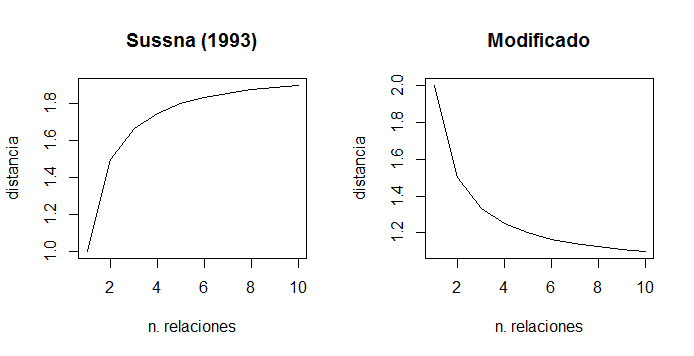
\includegraphics{sussnafail.png}
\caption[Evolución de la distancia entre conceptos según la formulación de Sussna (y corrección propuesta).]{Variación de la distancia asociada a una conexión en función del número relaciones
entre los elementos. A la izquierda los resultados según la formulación de
Sussna, a la derecha los resultados según la modificación propuesta. La línea roja
muestra la variación de la distancia cuando el concepto está en el primer nivel de
profundidad de la jerarquía y la azul cuando está a una profundidad de 10.}\label{4.model/i.recursos:fig-sussna-fail}\end{figure}

Al programar todas las medidas de distancia anteriores se han tenido en cuenta los siguientes
puntos:
\begin{itemize}
\item {} 
Todas utilizan la jerarquía de WordNet 3.1 construida con \code{WordNet-blast} haciendo uso
únicamente de las relaciones de hiponimia/hiperonima.

\item {} 
A las medidas basadas en el contenido de información que necesitaban de un \emph{corpus} se les
ha proporcionado los datos del \emph{corpus} SemCor expuesto anteriormente.

\item {} 
Todas estas medidas se han programado de tal forma que ofrezcan un valor de distancia
\(d\) o similaridad \(s\) comprendido en el intervalo \([0,1]\) tal que
se cumpla la relación
\begin{gather}
\begin{split}d(c_1, c_2) + s(c_1, c_2) = 1\end{split}\notag
\end{gather}
para cualquier par de conceptos \(c1\) y \(c2\) de la jerarquía. En algunos
casos la formulación estaba preparada para devolver este valor, en otros ha tenido
que calcularse el máximo valor posible dados los recursos utilizados (WordNet y SemCor)
para poder normalizar el resultado.

\end{itemize}

Gracias a estas consideraciones y, en especial, a la normalización realizada,
todas estas medidas pueden ser intercambiadas en el modelo de distancia entre grafos,
se pueden así comparar los resultados obtenidos con ellas.


\subsection{Distancia y jerarquía entre relaciones UNL}
\label{4.model/i.recursos:distancia-y-jerarquia-entre-relaciones-unl}
En la bibliografía no hemos encontrado ningún documento acerca de la distancia semántica entre
relaciones UNL, por lo que debemos proponer una. Para ello planteamos un modelo muy simple
basado en la jerarquía de relaciones que aparece en UNLWeb \footnote{
UNL Wiki. Universal Relations. \href{http://www.unlweb.net/wiki/Universal\_Relations}{http://www.unlweb.net/wiki/Universal\_Relations}
(accedido en junio de 2015)
} (ver \hyperref[4.model/i.recursos:table-unl-relations]{tabla  \ref*{4.model/i.recursos:table-unl-relations}}).

\begin{longtable}{|p{3cm}|p{4cm}|p{4cm}|}
\caption{Jerarquía de relaciones UNL según UNLWeb.}\label{4.model/i.recursos:table-unl-relations}\\
\hline
\endfirsthead

\multicolumn{1}{c}%
{{\textsf{\tablename\ \thetable{} -- proviene de la página anterior}}} \\
\hline
\endhead

\hline \multicolumn{1}{|r|}{{\textsf{Continúa en la página siguiente}}} \\ \hline
\endfoot

\endlastfoot


\begin{DUlineblock}{0em}
\item[] \textbf{agt}: agent
\item[] \textbf{and}: conjuntion
\item[] \textbf{aoj}: object of an attribute
\item[]
\begin{DUlineblock}{\DUlineblockindent}
\item[] \textbf{ant}: antonym, different from
\item[] \textbf{equ}: synonym, equal to
\item[] \textbf{fld}: field
\item[] \textbf{icl}: hyponym, a kind of
\item[] \textbf{iof}: example, instance of
\item[] \textbf{pof}: meronym, part of
\end{DUlineblock}
\item[] \textbf{ben}: beneficiary
\item[] \textbf{cnt}: content or theme
\item[] \textbf{con}: condition
\item[] \textbf{exp}: experiencer
\item[] \textbf{mod}: modifier
\item[]
\begin{DUlineblock}{\DUlineblockindent}
\item[] \textbf{mat}: material
\item[] \textbf{nam}: name
\item[] \textbf{pos}: possessor
\item[] \textbf{qua}: quantifier
\end{DUlineblock}
\item[] \textbf{obj}: patient
\item[]
\begin{DUlineblock}{\DUlineblockindent}
\item[] \textbf{opl}: objective place
\item[] \textbf{res}: result
\end{DUlineblock}
\item[] \textbf{or}: disjunction
\item[] \textbf{per}: proportion, rate, distribution or basis for a comparison
\item[]
\begin{DUlineblock}{\DUlineblockindent}
\item[] \textbf{bas}: basis for a comparison
\end{DUlineblock}
\item[] \textbf{plc}: location: physical or logical
\item[]
\begin{DUlineblock}{\DUlineblockindent}
\item[] \textbf{gol}: final place or state, destination
\item[] \textbf{lpl}: logical place, scene
\item[] \textbf{src}: initial place or state, origin
\item[] \textbf{via}: intermediate place, path
\end{DUlineblock}
\item[] \textbf{ptn}: partner
\end{DUlineblock}
\\
\hline
\begin{DUlineblock}{0em}
\item[] \textbf{tim}: time
\item[]
\begin{DUlineblock}{\DUlineblockindent}
\item[] \textbf{tmf}: initial time
\item[] \textbf{tmt}: final time
\item[] \textbf{dur}: duration
\item[]
\begin{DUlineblock}{\DUlineblockindent}
\item[] \textbf{coo}: co-occurrence
\end{DUlineblock}
\end{DUlineblock}
\item[] \textbf{man}: manner
\item[]
\begin{DUlineblock}{\DUlineblockindent}
\item[] \textbf{ins}: instrument or method
\item[]
\begin{DUlineblock}{\DUlineblockindent}
\item[] \textbf{met}: method
\end{DUlineblock}
\item[] \textbf{pur}: purpose
\end{DUlineblock}
\item[] \textbf{rsn}: reason
\item[] \textbf{seq}: consequence
\end{DUlineblock}
\\
\hline\end{longtable}


Proponemos un modelo según el cual dos relaciones son iguales si pertenecen a la misma
tipología de primer nivel (agt, and, aoj,...) y distintas en caso contrario (ver
\hyperref[4.model/i.recursos:table-unl-relations]{tabla  \ref*{4.model/i.recursos:table-unl-relations}}), así, sean dos relaciones, \(r_1\) y \(r_2\),
que conectan dos pares de conceptos equivalentes según la medida de similaridad entre
conceptos seleccionada, entonces:
\begin{gather}
\begin{split}s_r(r_1, r_2) = 1 - d_r(r_1, r_2) = \begin{cases}
1, & r_1 \equiv r_2\\
0.8, & \exists r_p \mid r_p \quad subsumes \quad \{r_1, r_2\}\\
0.2, & otherwise.
\end{cases}\end{split}\notag
\end{gather}
Como se puede observar la mínima similaridad entre dos relaciones es \(0.2\), se
considera así que la mera existencia de una relación entre dos mismos conceptos
indica un grado mínimo de similaridad.


\subsection{Algoritmo de McGregor}
\label{4.model/i.recursos:algoritmo-de-mcgregor}
El modelo que proponemos se basa en la búsqueda de máximos grafos comunes, es un problema
bastante tratado en la bibliografía. Existen dos aproximaciones muy frecuentes para la
resolución de este problema: convertirlo en un problema de búsqueda del máximo \emph{clique} o
realizar una búsqueda con retroceso.

El algoritmo propuesto por McGregor en 1982 \phantomsection\label{4.model/i.recursos:id18}{\hyperref[zreferences:mcgregor1982]{\emph{{[}54{]}}}} pertenece a los de búsqueda
con retroceso y según diferentes autores esta aproximación es más eficiente en grafos
dispersos \phantomsection\label{4.model/i.recursos:id19}{\hyperref[zreferences:bunke2002]{\emph{{[}13{]}}}} \phantomsection\label{4.model/i.recursos:id20}{\hyperref[zreferences:conte2007]{\emph{{[}19{]}}}} \phantomsection\label{4.model/i.recursos:id21}{\hyperref[zreferences:welling2011]{\emph{{[}97{]}}}}, como es el caso de
los grafos conceptuales.

Este algoritmo lo hemos incorporado a nuestro modelo utilizando la implementación disponible
en la librería \emph{graph} dentro de las Boost \footnote{
Boost Graph Library: McGregor Common Subgraphs. Boost C++ Libraries.
\href{http://www.boost.org/doc/libs/1\_58\_0/libs/graph/doc/mcgregor\_common\_subgraphs.html}{http://www.boost.org/doc/libs/1\_58\_0/libs/graph/doc/mcgregor\_common\_subgraphs.html}
(accedido en junio de 2015)
}, que además están programadas en C++.

La implementación disponible en la Boost nos permite aplicar con facilidad dos ideas
que perseguimos en el planteamiento de nuestro modelo:
\begin{itemize}
\item {} 
Podemos ejecutar el algoritmo con una función de comparación entre los nodos
de los grafo definida por nosotros mismos. Utilizaremos esta funcionalidad para
incorporar cualquiera de las medidas de distancia entre conceptos que ya hemos
expuesto, pero también para codificar el umbral de tolerancia entre ellos.

Nuestra función indicará al algoritmo McGregor de las Boost que dos nodos son
iguales cuando la distancia entre ellos sea menor que el umbral indicado:
\begin{gather}
\begin{split}c_1 \equiv c_2 \iff d_T(c_1, c_2) \leq t_c\end{split}\notag
\end{gather}
El mismo razonamiento lo utilizaremos para aplicar la distancia entre relaciones.

\item {} 
La librería también nos permite ejecutar el algoritmo de tal forma que podemos
acceder a todos los grafos que encuentra, aunque no sean el máximo grafo común;
esto nos permite almacenarlos todos ellos, algo que utilizaremos posteriormente en
nuestro modelo.

\end{itemize}


\section{El modelo}
\label{4.model/ii.modelo::doc}\label{4.model/ii.modelo:el-modelo}
Sean dos grafos conceptuales \(G_1\) y \(G_2\), nuestro objetivo es encontrar un
subgrafo \(H_1\) de \(G_1\) y un subgrafo \(H_2\) de \(G_2\) tal que
\(H_1\) y \(H_2\) sean isomorfos y maximicen la similaridad entre los grafos
de partida. Los subgrafos \(H_1\) y \(H_2\) no es necesario que sean conexos.

La correspondencia entre los subgrafos \(H_1\) y \(H_2\) se realiza a través de una
función de similaridad semántica entre conceptos \(s_C(c_i, c_j)\) y de similaridad entre
relaciones \(s_R(r_i, r_j)\) que se pueden configurar con un umbral de tolerancia entre
cada pareja de conceptos o relaciones, \(t_c\) y \(t_r\) respectivamente, en el
intervalo \([0, 1)\) donde \(0\) exige una correspondencia exacta y \(1\)
aceptaría como iguales cualquier pareja.

La búsqueda de los subgrafos \(H_1\) y \(H_2\) se realiza utilizando el algoritmo
McGregor y guardando todos los subgrafos comunes candidatos a ser máximo subgrafo común;
en un paso posterior se escoge de entre los candidatos el subconjunto que maximice la
similaridad entre los grafos de partida (no se consideran componentes formados por
un único nodo). Así:
\begin{gather}
\begin{split}sim(G_1, G_2) = argmax \sum_{i \in G_1, j \in G_2} sim(c_i, c_j) + sim(r_i, r_j)\end{split}\notag
\end{gather}
Este valor se normaliza teniendo en cuenta el valor máximo que podría alcanzar, el cual
se calcula considerando todos los ejes y conexiones de ambos grafos:
\begin{gather}
\begin{split}sim_{MAX}(G_1, G_2) = max(|G_1|, |G_2|) + max(e_{G_1}, e_{G_2})\end{split}\notag
\end{gather}
donde \(|G_i|\) representa la cardinalidad del grafo \(G_i\), es decir, el
número de nodos y \(e_{G_i}\) es el número de conexiones existentes en el
grafo \(G_i\).

Por lo tanto, el valor de similaridad se calcularía como
\begin{gather}
\begin{split}s(G_1, G_2) = \frac{sim(G_1, G_2)}{sim_{MAX}(G_1, G_2)}\end{split}\notag
\end{gather}
y tomará siempre valores en el intervalo \([0, 1]\).
\begin{figure}[htbp]
\centering
\capstart

\includegraphics{graphviz-ffa0b0859a1da950b25f6f683931cdabc9b29a30.pdf}
\caption{Grafos de ejemplo \(g_1\) (izda) y \(g_2\) (dcha).}\label{4.model/ii.modelo:fig-model-example-graph}\end{figure}

En la \hyperref[4.model/ii.modelo:fig-model-example-graph]{figura  \ref*{4.model/ii.modelo:fig-model-example-graph}} se muestran dos grafos que servirán de
ejemplo para ilustrar el modelo. En este caso no se han introducido etiquetas en las
relaciones para simplificar la representación.

El algoritmo de McGregor nos permitirá realizar la búsqueda del máximo grafo común
de una forma ordenada. Utilizando un nivel de tolerancia entre conceptos \(t_c=0\)
exigimos una correspondencia exacta entre ellos y obtenemos el resultado de la
\hyperref[4.model/ii.modelo:fig-model-example-mcs1]{figura  \ref*{4.model/ii.modelo:fig-model-example-mcs1}}.

En dicha figura se ha marcado en color los nodos y las relaciones que pertenecen a
la solución de nuestro algoritmo: en este caso estaría formada por dos subgrafos
(el rojo se correspondenría con el máximo grafo común) y ambos contribuyen al
valor de similaridad. A pesar de que hay otros nodos que también están presentes
en ambos grafos (como el nodo \(A\)) este no forma parte de la solución puesto
que está aislado y ya hemos comentado que solo se consideran aquellos componentes que
estén formados por un mínimo de dos nodos (como es el caso de la pareja \(G, H\)).
\begin{figure}[htbp]
\centering
\capstart

\includegraphics{graphviz-0e7f07f7f1ad51b62d383754a0177a5750a46883.pdf}
\caption{Máximo grafo común de \(g_1\) y \(g_2\) con nivel de tolerancia, \(t_c=0\) (exige correspondencia exacta en los nodos).}\label{4.model/ii.modelo:fig-model-example-mcs1}\end{figure}

El valor de similaridad calculado por el modelo sería la suma de las similaridades de
los dos subgrafos coincidentes, entre la máxima posible:
\begin{gather}
\begin{split}s(g_1, g_2)_{t_c=0}=\frac{s_{g_{ROJO}} + s_{g_{AZUL}}}{max(|g_1|, |g_2|) + max(e_{g_1}, e_{g_2})}\end{split}\notag
\end{gather}
y como hemos exigido una correspondencia exacta (\(t_c=0\)) entonces la similaridad
entre cada pareja de nodos será la máxima (la unidad) y podemos calcular el valor
resultante de forma sencilla:
\begin{gather}
\begin{split}s(g_1, g_2)_{t_c=0}=\frac{|g_{ROJO}| + |g_{AZUL}| + e_{g_{ROJO}} + e_{g_{AZUL}}}{|g_1| + e_{g_1}} = \frac{4 + 2 + 4 + 1}{9 + 11} = \frac{11}{20}\end{split}\notag
\end{gather}
Si aumentamos la tolerancia entre conceptos, \(t_c\), ocurrirá que nodos que
antes no aparecían en la solución comiencen a hacerlo puesto que su distancia semántica
según la medida elegida será menor que el umbral de tolerancia utilizado como
parámetro. En concreto, si hacemos que el valor \(t_c\) verifique que
\begin{gather}
\begin{split}t_c \geq d(I, i)  \Rightarrow  t_c \geq 1 - s(I, i)\end{split}\notag
\end{gather}
entonces la solución de nuestro algoritmo será la mostrada en la
\hyperref[4.model/ii.modelo:fig-model-example-mcs2]{figura  \ref*{4.model/ii.modelo:fig-model-example-mcs2}} donde se verifica que \(I \approx i\) y se
incorporan a la solución en el subgrafo azul.
\begin{figure}[htbp]
\centering
\capstart

\includegraphics{graphviz-7fc55e444d54889cb878f9c556c18f2fb099ac32.pdf}
\caption{Máximo grafo común de \(g_1\) y \(g_2\) con nivel de toleracia, \(t_c \geq d(I, i)\).}\label{4.model/ii.modelo:fig-model-example-mcs2}\end{figure}

El valor de similaridad será mayor que el calculado anteriormente, en concreto se
incrementará debido a la similaridad aportada por la nueva conexión que pasa a
formar parte de la solución y la similaridad entre los nodos:
\begin{gather}
\begin{split}s(g_1, g_2)_{t_c \geq d(I,i)}= s(g_1, g_2)_{t_c=0} + \frac{1 + s(I, i)}{20} = \frac{12 + s(I, i)}{20}\end{split}\notag
\end{gather}
El valor de similaridad se incrementa a medida que aumentamos los umbrales de
tolerancia. En grafos donde la correspondencia entre nodos no sea tan evidente al
aumentar el umbral de tolerancia van a aparecer subgrafos
superpuestos, en estos casos el modelo deberá explorar todas las combinaciones posibles
para quedarse con la solución que maximice la similaridad.
\newpage

\chapter{Pruebas}
\label{5.pruebas/index::doc}\label{5.pruebas/index:pruebas}
Con el objetivo de probar el modelo se ha diseñado un experimento que permite
contrastar textos generados por dos sistemas diferentes de traducción automática
para evaluar la distancia con respecto al texto original.

El experimento consiste en comparar un conjunto de grafos UNL
(convertidos a grafos cuyos nodos son \emph{synsets} de WordNet) extraídos de un
documento perteneciente al Forum Universal de las Culturas 2004 \footnote{
Fòrum Universal de les Cultures.
\href{http://www.barcelona2004.org/www.barcelona2004.org/cat/index.html}{http://www.barcelona2004.org/www.barcelona2004.org/cat/index.html}
(accedida en junio de 2015)
} celebrado
en Barcelona. La comparación se realizará contra los grafos resultantes de traducir
estas oraciones al español y de vuelta al inglés utilizando software de traducción
disponible en internet.
\begin{figure}[htbp]
\centering
\capstart

\includegraphics{graphviz-dfc284b51cbf5a3de58db7f60d1f3b03491e90c9.pdf}
\caption[Metodología elaborada para obtener el conjunto de datos utilizado en la experimentación del modelo.]{Metodología elaborada para obtener el conjunto de datos utilizado en la experimentación del modelo. Se muestra la obtención de la distancia entre el grafo original y el obtenido a partir de la traducción de Yandex.}\label{5.pruebas/index:fig-experiment-layout}\end{figure}

En la \hyperref[5.pruebas/index:fig-experiment-layout]{figura  \ref*{5.pruebas/index:fig-experiment-layout}} se muestra el proceso seguido para cada
una de las oraciones seleccionadas y los actores que intervienen en la generación de
los recursos; como ya se indicó en la {\hyperref[2.problem/index:planteamiento-problema]{\emph{\DUspan{}{sección 3.3}}}}, al
carecer de tiempo y medios para generar un conjunto de datos adecuado, ha sido
necesario crearlos \emph{ex profeso} para este trabajo \footnote{
En el {\hyperref[appendix-data:appendix-data]{\emph{\DUspan{}{Apéndice A}}}} se encuentran disponibles todos los datos
utilizados para la realización del experimento.
}. Se asume así que los resultados
deben ser revisados con un enfoque más científico, pero creemos que los datos generados
de esta forma pueden servir para realizar una primera evaluación del modelo.


\section{Metodología}
\label{5.pruebas/index:metodologia}
Ilustraremos la metodología mostrada en la \hyperref[5.pruebas/index:fig-experiment-layout]{figura  \ref*{5.pruebas/index:fig-experiment-layout}} con
el ejemplo número 3 del \emph{dataset} que hemos elaborado. El procedimiento se detalla
en los siguientes apartados.


\subsection{Datos de partida: oración y grafo UNL}
\label{5.pruebas/index:datos-de-partida-oracion-y-grafo-unl}
En el documento al que hemos hecho referencia anteriormente tenemos disponibles las
oraciones en inglés y su transcripción como grafo UNL. La oración sobre la que
trabajaremos es la siguiente,
\begin{description}
\item[{Ejemplo 3}] \leavevmode
: \emph{These concepts are essential for advancing towards a sustainable, more human world agenda, and they will undoubtedly continue to be relevant for many years to come.}

\end{description}

cuyo grafo UNL se muestra en el \hyperref[5.pruebas/index:code-example-unl-3]{listado  \ref*{5.pruebas/index:code-example-unl-3}}.

\begin{literal-block}
\caption{Codificación UNL original de la oración ejemplo 3.}
\begin{Verbatim}[commandchars=\\\{\}]
[S]
obj(continue(icl\PYGZgt{}occur).@entry,:01)
mod:01(concept(icl\PYGZgt{}logic).@entry.@pl,this)
man(continue(icl\PYGZgt{}occur).@entry,undoubtedly(icl\PYGZgt{}man))
gol(continue(icl\PYGZgt{}occur).@entry,:02)
aoj:02(relevant(mod\PYGZlt{}thing).@entry,:01)
dur:02(relevant(mod\PYGZlt{}thing).@entry,year(icl\PYGZgt{}time).@pl)
mod:02(year(icl\PYGZgt{}time).@pl,many)
mod:02(year(icl\PYGZgt{}time).@pl,forthcoming(mod\PYGZlt{}thing))
and(continue(icl\PYGZgt{}occur).@entry,essential(mod\PYGZlt{}thing))
aoj(essential(mod\PYGZlt{}thing),:01)
pur(essential(mod\PYGZlt{}thing),advance(icl\PYGZgt{}progress(icl\PYGZgt{}do)))
man(advance(icl\PYGZgt{}progress(icl\PYGZgt{}do)),towards)
obj(towards,:03)
mod:03(agenda(icl\PYGZgt{}programme).@entry,world(mod\PYGZlt{}thing))
mod(:03,human(mod\PYGZlt{}thing))
man(human(mod\PYGZlt{}thing),more)
and(human(mod\PYGZlt{}thing),sustainable(mod\PYGZlt{}thing))
[/S]
\end{Verbatim}
\phantomsection\label{5.pruebas/index:code-example-unl-3}
\end{literal-block}


\subsection{Traducción a idioma intermedio}
\label{5.pruebas/index:traduccion-a-idioma-intermedio}
El siguiente paso consiste en traducir la oración original a un segundo idioma que
servirá de punto de partida para las traducciones generadas por los sistemas que vamos
a comparar.

En nuestro caso el idioma intermedio será el español, y la traducción la generaremos
utilizando el sistema Systrans \footnote{
SYSTRANet – Online translation software and tools – Dictionary.
\href{http://www.systranet.com/dictionary/english-spanish}{http://www.systranet.com/dictionary/english-spanish} (accedido en junio
de 2015)
}:
\begin{quote}

\textbf{Systrans}: Estos conceptos son esenciales para avanzar hacia un orden del día sostenible, más humano del mundo, y continuarán indudablemente siendo relevantes durante muchos años de venir.
\end{quote}

Como podemos ver, este sistema ya ha introducido alguna variación respecto al contenido
original, incluso la corrección gramatical de la oración parece estar comprometida.


\subsection{Traducción al idioma original}
\label{5.pruebas/index:traduccion-al-idioma-original}
La oración en español es traducida nuevamente al idioma de partida (inglés) utilizando
dos sistemas de traducción automática: Google \footnote{
Traductor de Google. \href{https://translate.google.es}{https://translate.google.es} (accedido en junio de 2015)
} y Yandex \footnote{
Yandex.Translate. \href{https://translate.yandex.com/}{https://translate.yandex.com/} (accedido en junio de 2015)
}, con los que obtenemos
los siguientes resultados:
\begin{quote}

\textbf{Google}: \emph{These concepts are essential in order to move towards a more sustainable day human world, and will undoubtedly continue to be relevant for many years to come.}

\textbf{Yandex}: \emph{These concepts are essential for progress towards an agenda for sustainable, more human world, and undoubtedly will continue to remain relevant for many years to come.}
\end{quote}

Leyendo las oraciones resultantes podemos observar cómo las traducciones no son idénticas
entre ellas y se han alejado del contenido semántico original. Nuestro modelo trabajará con
estos datos para obtener una medida de distancia entre las traducciones y la oración
original.


\subsection{Identificación de los \emph{synsets} de WordNet}
\label{5.pruebas/index:identificacion-de-los-synsets-de-wordnet}
Como hemos indicado, la ontología UNL no está disponible, por lo que la manera
de utilizar las medidas de distancia que hemos expuesto en el estado del arte debe
ser a través de la jerarquía de conceptos de WordNet. Para ello hemos tenido que
identificar cada concepto expresado por las UWs con un \emph{synset} concreto en WordNet.

Este proceso se ha realizado manualmente y, con total seguridad, el autor está
introduciendo una primera
desviación semántica entre la oración original y el grafo base para la comparación; no
obstante, se ha tenido la precaución de que siempre que aparecen los mismos conceptos
se sustituye por el mismo \emph{synset}.

De este modo, el grafo UNL original, se convierte en el grafo mostrado en el
\hyperref[5.pruebas/index:code-example-original-3]{listado  \ref*{5.pruebas/index:code-example-original-3}} que también se muestra en la
\hyperref[5.pruebas/index:sample03-original]{figura  \ref*{5.pruebas/index:sample03-original}}.

\begin{literal-block}
\caption{Codificación utilizando los \emph{synsets} de WordNet de la oración ejemplo 7.}
\begin{Verbatim}[commandchars=\\\{\}]
\PYGZob{}unl\PYGZcb{}
obj(continue\PYGZpc{}2:42:01::, concept\PYGZpc{}1:09:00::)
man(continue\PYGZpc{}2:42:01::, undoubtedly\PYGZpc{}4:02:00::)
gol(continue\PYGZpc{}2:42:01::, be\PYGZpc{}2:42:03::)
aoj(be\PYGZpc{}2:42:03::, concept\PYGZpc{}1:09:00::)
obj(be\PYGZpc{}2:42:03::, relevant\PYGZpc{}3:00:00::)
dur(relevant\PYGZpc{}3:00:00::, year\PYGZpc{}1:28:01::)
mod(year\PYGZpc{}1:28:01::, many\PYGZpc{}3:00:00::)
mod(year\PYGZpc{}1:28:01::, forthcoming\PYGZpc{}5:00:00:future:00)
and(continue\PYGZpc{}2:42:01::, essential\PYGZpc{}3:00:00:necessary:00)
aoj(essential\PYGZpc{}3:00:00:necessary:00, concept\PYGZpc{}1:09:00::)
pur(essential\PYGZpc{}3:00:00:necessary:00, advance\PYGZpc{}2:38:00::)
plc(advance\PYGZpc{}2:38:00::, agenda\PYGZpc{}1:10:00::)
mod(agenda\PYGZpc{}1:10:00::, world\PYGZpc{}1:14:02::)
mod(agenda\PYGZpc{}1:10:00::, human\PYGZpc{}3:01:00::)
man(human\PYGZpc{}3:01:00::, more\PYGZpc{}4:02:00::)
and(human\PYGZpc{}3:01:00::, sustainable\PYGZpc{}3:01:00::)
\PYGZob{}/unl\PYGZcb{}
\end{Verbatim}
\phantomsection\label{5.pruebas/index:code-example-original-3}
\end{literal-block}
\begin{figure}[htbp]
\centering
\capstart

\scalebox{1.000000}{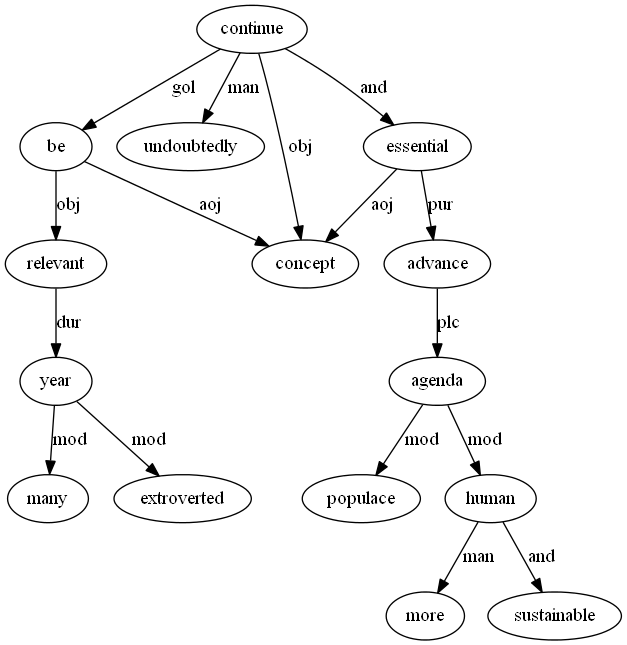
\includegraphics[width=1.000\linewidth]{sample03_original.png}}
\caption[Grafo correspondiente al ejemplo \#3 utilizado en el experimento.]{Grafo correspondiente al ejemplo \#3 utilizado en el experimento (se muestran
únicamente las \emph{headwords} correspondientes a cada concepto).}\label{5.pruebas/index:sample03-original}\end{figure}

La conversión de los conceptos UNL expresados en las UWs en los \emph{synsets} de WordNet
se ha realizado utilizando el buscador de WordNet accesible en la página web de la Universidad
de Princeton \footnote{
WordNet Search - 3.1. \href{http://wordnetweb.princeton.edu/perl/webwn}{http://wordnetweb.princeton.edu/perl/webwn} (accedido en
junio de 2015).
}, de entre todas las opciones proporcionadas para cada palabra se
ha seleccionado el concepto más próximo dentro de la categoría gramatical adecuada.

El mismo procedimiento se ha realizado para convertir las traducciones de Google y
Yandex en grafos. Los resultados obtenidos se pueden consultar en los listados
\hyperref[5.pruebas/index:code-example-google-3]{ \ref*{5.pruebas/index:code-example-google-3}} y \hyperref[5.pruebas/index:code-example-yandex-3]{ \ref*{5.pruebas/index:code-example-yandex-3}} y las figuras
\hyperref[5.pruebas/index:sample03-google]{ \ref*{5.pruebas/index:sample03-google}} y \hyperref[5.pruebas/index:sample03-yandex]{ \ref*{5.pruebas/index:sample03-yandex}}.

\begin{literal-block}
\caption{Codificación utilizando los \emph{synsets} de WordNet del resultado de la traducción de la oración ejemplo 3 mediante el sistema Google.}
\begin{Verbatim}[commandchars=\\\{\}]
 \PYGZob{}unl\PYGZcb{}
 obj(continue\PYGZpc{}2:42:01::, concept\PYGZpc{}1:09:00::)
 man(continue\PYGZpc{}2:42:01::, undoubtedly\PYGZpc{}4:02:00::)
 gol(continue\PYGZpc{}2:42:01::, be\PYGZpc{}2:42:03::)
 aoj(be\PYGZpc{}2:42:03::, concept\PYGZpc{}1:09:00::)
 obj(be\PYGZpc{}2:42:03::, relevant\PYGZpc{}3:00:00::)
 dur(relevant\PYGZpc{}3:00:00::, year\PYGZpc{}1:28:01::)
 mod(year\PYGZpc{}1:28:01::, many\PYGZpc{}3:00:00::)
 mod(year\PYGZpc{}1:28:01::, forthcoming\PYGZpc{}5:00:00:future:00)
 and(continue\PYGZpc{}2:42:01::, essential\PYGZpc{}3:00:00:necessary:00)
 aoj(essential\PYGZpc{}3:00:00:necessary:00, concept\PYGZpc{}1:09:00::)
 pur(essential\PYGZpc{}3:00:00:necessary:00, move\PYGZpc{}2:41:01::)
 plc(move\PYGZpc{}2:41:01::, day\PYGZpc{}1:26:00::)
 mod(day\PYGZpc{}1:26:00::, world\PYGZpc{}1:14:02::)
 mod(day\PYGZpc{}1:26:00::, human\PYGZpc{}3:01:00::)
 mod(day\PYGZpc{}1:26:00::, sustainable\PYGZpc{}3:01:00::)
 \PYGZob{}/unl\PYGZcb{}
\end{Verbatim}
\phantomsection\label{5.pruebas/index:code-example-google-3}
\end{literal-block}
\begin{figure}[htbp]
\centering
\capstart

\scalebox{1.000000}{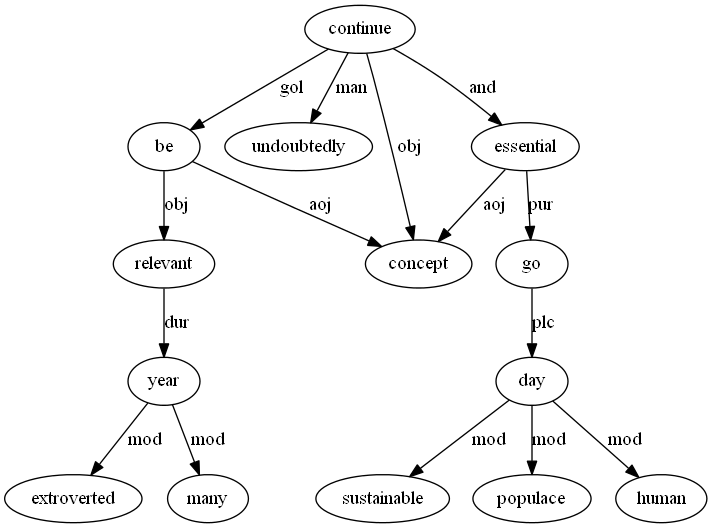
\includegraphics[width=1.000\linewidth]{sample03_google.png}}
\caption{Grafo correspondiente a la traducción de Google del ejemplo \#3.}\label{5.pruebas/index:sample03-google}\end{figure}

\begin{literal-block}
\caption{Codificación utilizando los \emph{synsets} de WordNet del resultado de la traducción de la oración ejemplo 3 mediante el sistema Yandex.}
\begin{Verbatim}[commandchars=\\\{\}]
 \PYGZob{}unl\PYGZcb{}
 obj(continue\PYGZpc{}2:42:01::, concept\PYGZpc{}1:09:00::)
 man(continue\PYGZpc{}2:42:01::, undoubtedly\PYGZpc{}4:02:00::)
 gol(continue\PYGZpc{}2:42:01::, be\PYGZpc{}2:42:03::)
 aoj(be\PYGZpc{}2:42:03::, concept\PYGZpc{}1:09:00::)
 obj(be\PYGZpc{}2:42:03::, relevant\PYGZpc{}3:00:00::)
 dur(relevant\PYGZpc{}3:00:00::, year\PYGZpc{}1:28:01::)
 mod(year\PYGZpc{}1:28:01::, many\PYGZpc{}3:00:00::)
 mod(year\PYGZpc{}1:28:01::, forthcoming\PYGZpc{}5:00:00:future:00)
 and(continue\PYGZpc{}2:42:01::, essential\PYGZpc{}3:00:00:necessary:00)
 aoj(essential\PYGZpc{}3:00:00:necessary:00, concept\PYGZpc{}1:09:00::)
 pur(essential\PYGZpc{}3:00:00:necessary:00, progress\PYGZpc{}2:30:00::)
 plc(progress\PYGZpc{}2:30:00::, agenda\PYGZpc{}1:10:00::)
 pur(agenda\PYGZpc{}1:10:00::, world\PYGZpc{}1:14:02::)
 mod(world\PYGZpc{}1:14:02::, human\PYGZpc{}3:01:00::)
 man(human\PYGZpc{}3:01:00::, more\PYGZpc{}4:02:00::)
 and(world\PYGZpc{}1:14:02::, sustainable\PYGZpc{}3:01:00::)
 \PYGZob{}/unl\PYGZcb{}
\end{Verbatim}
\phantomsection\label{5.pruebas/index:code-example-yandex-3}
\end{literal-block}
\begin{figure}[htbp]
\centering
\capstart

\scalebox{1.000000}{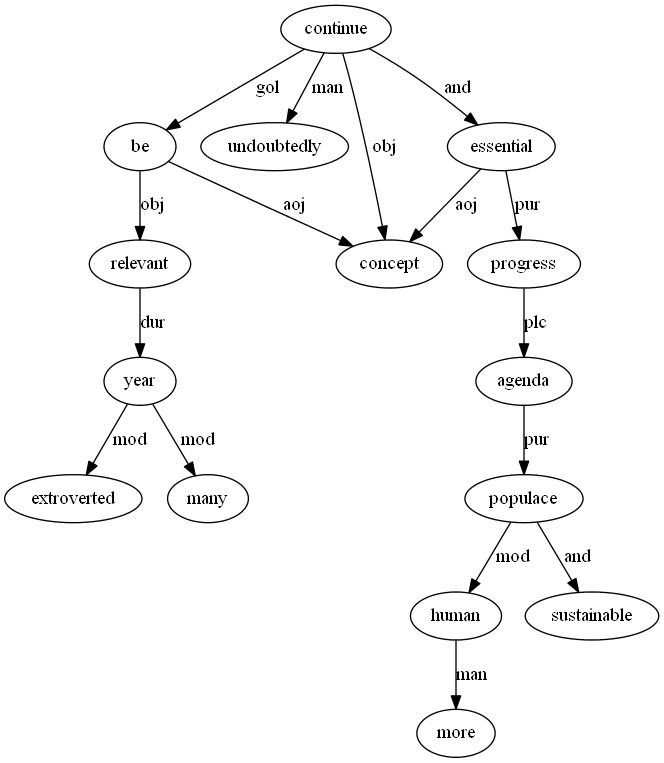
\includegraphics[width=1.000\linewidth]{sample03_yandex.png}}
\caption{Grafo correspondiente a la traducción de Yandex del ejemplo \#3.}\label{5.pruebas/index:sample03-yandex}\end{figure}


\subsection{Ejecución del modelo}
\label{5.pruebas/index:ejecucion-del-modelo}
Una vez que se tienen disponibles los grafos generados por los traductores, se
realiza la comparación de cada uno de ellos con el grafo de referencia para calcular
la distancia semántica introducida por cada uno de los sistemas de traducción y
poder evaluar su rendimiento de forma automática.

A la hora de ejecutar el modelo, el usuario debe seleccionar algunos parámetros:
\begin{itemize}
\item {} 
Algoritmo para el cálculo de la distancia entre conceptos.

\item {} 
Tolerancia en la comparación entre conceptos.

\item {} 
Tolerancia en la comparación entre relaciones.

\end{itemize}
\begin{figure}[htbp]
\centering
\capstart

\scalebox{1.000000}{\includegraphics[width=1.000\linewidth]{measures-yandex-synset.png}}
\caption[Similaridad entre el grafo original y el grafo generado por el traductor de Yandex.]{Similaridad entre el grafo original y el grafo generado por el traductor de Yandex en función de la tolerancia entre conceptos. Se muestra la evolución de este valor para todas las métricas de distancia incorporadas en el algoritmo.}\label{5.pruebas/index:sample03-measures-yandex-synset}\end{figure}
\begin{figure}[htbp]
\centering
\capstart

\scalebox{1.000000}{\includegraphics[width=1.000\linewidth]{measures-google-synset.png}}
\caption[Similaridad entre el grafo original y el grafo generado por el traductor de Google.]{Similaridad entre el grafo original y el grafo generado por el traductor de Google en función de la tolerancia entre conceptos. Se muestra la evolución de este valor para todas las métricas de distancia incorporadas en el algoritmo.}\label{5.pruebas/index:sample03-measures-google-synset}\end{figure}

En la \hyperref[5.pruebas/index:sample03-measures-yandex-synset]{figura  \ref*{5.pruebas/index:sample03-measures-yandex-synset}} y en la
\hyperref[5.pruebas/index:sample03-measures-google-synset]{figura  \ref*{5.pruebas/index:sample03-measures-google-synset}}
se muestra el valor calculado de similaridad para estos grafos utilizando todas
las medidas de similaridad/distancia entre conceptos disponibles y para
diferentes valores de tolerancia entre conceptos, \(t_c \in [0.0, 0.9]\).

Una gráfica similar se ha realizado fijando un valor de tolerancia para la
distancia entre conceptos y variando la tolerancia entre relaciones, no se ha
reproducido aquí porque no se produce ninguna variación en el valor de
similaridad.

Tanto en la comparación con el grafo generado por el traductor de Google como
en el de Yandex, existe un umbral de \(t_c\) en el que se produce un salto
en el valor de similaridad entre los grafos para la mayoría de los algoritmos
de distancia semántica. Una inspección detallada de los resultados nos permite
encontrar el par de palabras que empiezan a ser equivalentes cuando la tolerancia
supera cierto umbral.

En la comparación entre la traducción de Google y el grafo original, el par de
palabras que pasa a ser considerado equivalente es \code{agenda} y \code{day}, en cada
caso con un valor de similaridad diferente:
\begin{itemize}
\item {} 
Sussna \(s_c(agenda, day) = 0.828666\)

\item {} 
Shortest-path \(s_c(agenda, day) = 0.684211\)

\item {} 
Leacock-Chodorow: \(s_c(agenda, day) = 0.31688\)

\item {} 
Wu-Palmer \(s_c(agenda, day) = 0.142857\)

\item {} 
Resnik \(s_c(agenda, day) = 0.122799\)

\item {} 
Jiang-Conrath \(s_c(agenda, day) < 0.1\)

\item {} 
Lin \(s_c(agenda, day) < 0.1\)

\end{itemize}

En el caso de la traducción de Yandex el par de palabras que se incorpora al
máximo grafo común es \code{agenda} y \code{populace}, con los siguientes valores:
\begin{itemize}
\item {} 
Sussna \(s_c(agenda, populace) = 0.85633\)

\item {} 
Shortest-path \(s_c(agenda, populace) = 0.763158\)

\item {} 
Leacock-Chodorow \(s_c(agenda, populace) = 0.395966\)

\item {} 
Wu-Palmer \(s_c(agenda, populace) = 0.181818\)

\item {} 
Resnik \(s_c(agenda, populace) = 0.122799\)

\item {} 
Jiang-Conrath \(s_c(agenda, populace) < 0.1\)

\item {} 
Lin \(s_c(agenda, populace) < 0.1\)

\end{itemize}

Como consecuencia de la incorporación de un nuevo nodo al grafo resultante,
se añaden nuevas conexiones con sus valores de similaridad que incrementan
el valor calculado para la pareja de grafos.
\begin{figure}[htbp]
\centering
\capstart

\scalebox{1.000000}{\includegraphics[width=1.000\linewidth]{sussna-synset_tol-00.png}}
\caption{Conjunto de nodos y relaciones equivalentes en la comparación entre el grafo original y las traducciones de Google (en rojo) y Yandex (azul), cuando \(t_c = 0\).}\label{5.pruebas/index:sample03-sussna-synset-tol-0}\end{figure}
\begin{figure}[htbp]
\centering
\capstart

\scalebox{1.000000}{\includegraphics[width=1.000\linewidth]{sussna-synset_tol-09.png}}
\caption{Conjunto de nodos y relaciones equivalentes en la comparación entre el grafo original y las traducciones de Google (en rojo) y Yandex (azul), con tolerancia entre conceptos \(t_c = 0.9\).}\label{5.pruebas/index:id13}\end{figure}


\subsection{Valor de similaridad}
\label{5.pruebas/index:valor-de-similaridad}
Puesto que se dispone de varios algoritmos de medida de similaridad entre conceptos,
para calcular el valor final de similaridad entre los grafos podemos utilizar la media
de todos ellos, de este modo se obtiene un resultado como el que se muestra en la
\hyperref[5.pruebas/index:sample03-relation-tol-0]{figura  \ref*{5.pruebas/index:sample03-relation-tol-0}}: el valor de similaridad muestra una incremento
monótono conforme la tolerancia entre los conceptos aumenta, que es lo que cabría
esperar y que hemos comentado al exponer el modelo.
\begin{figure}[htbp]
\centering
\capstart

\scalebox{1.000000}{\includegraphics[width=1.000\linewidth]{synset_tol-relation_tol-0.png}}
\caption{Similaridad semántica entre el grafo original y los grafos correspondientes a las traducciones realizadas con Google (rojo) y Yandex (azul) en función de la tolerancia \(t_c\) entre conceptos (intervalo de confianza 95\%).}\label{5.pruebas/index:sample03-relation-tol-0}\end{figure}

En este caso concreto, el algoritmo indica que la distancia semántica es menor en el
caso de la traducción de Yandex que en la de Google; un conjunto de oraciones
etiquetado adecuadamente (probablemente fuera necesario realizarlo manualmente)
nos podría servir para valorar el desempeño de los traductores.


\section{Resultados}
\label{5.pruebas/index:resultados}
Para la experimentacion se ha preparado un \emph{dataset} con 10 oraciones extraídas del
documento del Forum Universal de las Culturas de Barcelona 2004 y traducidas utilizando
los servicios indicados anteriormente. El conjunto completo de oraciones se incluye a
continuación; la codificacion original, así como las correspondencias con WordNet y
la representación gráfica tanto del original como de las traducciones puede
consultarse en el \emph{dataset} completo que se adjunta en el {\hyperref[appendix-data:appendix-data]{\emph{\DUspan{}{Apéndice A}}}}.
\begin{description}
\item[{Ejemplo 1}] \leavevmode
: \emph{The Universal Forum of Cultures will be held from April 23 to September 24, 2004, and will include exhibitions, debates and festivals to celebrate cultural diversity throughout the world.}

\textbf{Systrans}: El foro universal de culturas será sostenido del 23 de abril al 24 de septiembre de 2004, e incluirá exposiciones, discusiones y festivales para celebrar diversidad cultural en el mundo entero.

\textbf{Google}: \emph{The Universal Forum of Cultures will be held from April 23 to September 24, 2004, and will include exhibitions, debates and festivals to celebrate cultural diversity in the world.}

\textbf{Yandex}: \emph{The universal forum of cultures will be held from April 23 to September 24, 2004, and will include exhibitions, discussions, and festivals that celebrate cultural diversity in the world.}

\end{description}
\begin{figure}[htbp]
\centering
\capstart

\scalebox{1.000000}{\includegraphics[width=1.000\linewidth]{synset_tol-relation_tol-01.png}}
\caption{Similaridad semántica entre el grafo original y las traducciones realizadas con Google (rojo) y Yandex (azul) en función de la tolerancia entre conceptos (intervalo de confianza 95\%) en el ejemplo 1.}\label{5.pruebas/index:sample01-relation-tol-0}\end{figure}
\begin{description}
\item[{Ejemplo 2}] \leavevmode
: \emph{In their 29th General Conference, the 186 member states of the Unesco ratified their unanimous support of the project, jointly organized by the Spanish government, the Catalan autonomous government and the Barcelona City Council.}

\textbf{Systrans}: En su 29na conferencia general, los 186 Estados miembros de la UNESCO ratificaron su ayuda unánime del proyecto, organizada en común por el gobierno español, el gobierno autónomo catalán y el Ayuntamiento de Barcelona.

\textbf{Google}: \emph{In its 29th general conference, the 186 Member States of UNESCO unanimously reaffirmed their support of the project, organized jointly by the Spanish government, the Catalan Autonomous Government and the City of Barcelona.}

\textbf{Yandex}: \emph{In your 29na general conference, the 186 member States of UNESCO have ratified their unanimous support of the project, organized jointly by the Spanish government, the autonomous government of catalonia and the Barcelona city Council.}

\end{description}
\begin{figure}[htbp]
\centering
\capstart

\scalebox{1.000000}{\includegraphics[width=1.000\linewidth]{synset_tol-relation_tol-02.png}}
\caption{Similaridad semántica entre el grafo original y las traducciones realizadas con Google (rojo) y Yandex (azul) en función de la tolerancia entre conceptos (intervalo de confianza 95\%) en el ejemplo 2.}\label{5.pruebas/index:sample02-relation-tol-0}\end{figure}
\begin{description}
\item[{Ejemplo 3}] \leavevmode
: \emph{These concepts are essential for advancing towards a sustainable, more human world agenda, and they will undoubtedly continue to be relevant for many years to come}

\textbf{Systrans}: Estos conceptos son esenciales para avanzar hacia un orden del día sostenible, más humano del mundo, y continuarán indudablemente siendo relevantes durante muchos años de venir

\textbf{Google}: \emph{These concepts are essential in order to move towards a more sustainable day human world, and will undoubtedly continue to be relevant for many years to come}

\textbf{Yandex}: \emph{These concepts are essential for progress towards an agenda for sustainable, more human world, and undoubtedly will continue to remain relevant for many years to come}

\item[{Ejemplo 4}] \leavevmode
: \emph{Knowledge of other cultures is essential for establishing a constructive dialogue between different communities.}

\textbf{Systrans}: El conocimiento de otras culturas es esencial para establecer un diálogo constructivo entre diversas comunidades.

\textbf{Google}: \emph{Knowledge of other cultures is essential to establish a constructive dialogue between different communities.}

\textbf{Yandex}: \emph{The knowledge of other cultures is essential to establish a constructive dialogue between various communities.}

\end{description}
\begin{figure}[htbp]
\centering
\capstart

\scalebox{1.000000}{\includegraphics[width=1.000\linewidth]{synset_tol-relation_tol-03.png}}
\caption{Similaridad semántica entre el grafo original y las traducciones realizadas con Google (rojo) y Yandex (azul) en función de la tolerancia entre conceptos (intervalo de confianza 95\%) en el ejemplo 4.}\label{5.pruebas/index:sample04-relation-tol-0}\end{figure}
\begin{description}
\item[{Ejemplo 5}] \leavevmode
: \emph{This knowledge implies reflection about the common ground between all individuals as well as the qualities that differentiate them.}

\textbf{Systrans}: Este conocimiento implica la reflexión sobre el terreno común entre todos los individuos así como las calidades que las distingan.

\textbf{Google}: \emph{This knowledge involves reflection on the common ground between all individuals and the qualities that distinguish them.}

\textbf{Yandex}: \emph{This knowledge implies reflection on the common ground between all individuals as well as the qualities that distinguish them.}

\end{description}
\begin{figure}[htbp]
\centering
\capstart

\scalebox{1.000000}{\includegraphics[width=1.000\linewidth]{synset_tol-relation_tol-04.png}}
\caption{Similaridad semántica entre el grafo original y las traducciones realizadas con Google (rojo) y Yandex (azul) en función de la tolerancia entre conceptos (intervalo de confianza 95\%) en el ejemplo 5.}\label{5.pruebas/index:sample05-relation-tol-0}\end{figure}
\begin{description}
\item[{Ejemplo 6}] \leavevmode
: \emph{The Forum strives to foster the kind of understanding and respect capable of increasing both our appreciation of our human environment and our ability to work together to make the world a better place.}

\textbf{Systrans}: El foro se esfuerza fomentar la clase de comprensión y respetar capaz de aumentar nuestro aprecio de nuestro ambiente humano y nuestra capacidad de trabajar junto para hacer el mundo un mejor lugar.

\textbf{Google}: \emph{The forum strives to promote the kind of understanding and respect able to increase our appreciation of our human environment and our ability to work together to make the world a better place.}

\textbf{Yandex}: \emph{The forum strives to foster the kind of understanding and respect able to increase our appreciation of our human environment and our ability to work together to make the world a better place.}

\end{description}
\begin{figure}[htbp]
\centering
\capstart

\scalebox{1.000000}{\includegraphics[width=1.000\linewidth]{synset_tol-relation_tol-05.png}}
\caption{Similaridad semántica entre el grafo original y las traducciones realizadas con Google (rojo) y Yandex (azul) en función de la tolerancia entre conceptos (intervalo de confianza 95\%) en el ejemplo 6.}\label{5.pruebas/index:sample06-relation-tol-0}\end{figure}
\begin{description}
\item[{Ejemplo 7}] \leavevmode
: \emph{Sustainable Development satisfies the needs of the present without compromising future generations' abilities to satisfy theirs, and is based on the natural environment's capacity to provide for humankind.}

\textbf{Systrans}: El desarrollo sostenible satisface las necesidades del presente sin las capacidades de las futuras generaciones de compromiso de satisfacer el suyo, y se basa en la capacidad del ambiente natural de prever humanidad.

\textbf{Google}: \emph{Sustainable development meets the needs of the present without the ability of future generations to meet his commitment, and is based on the ability of the natural environment to provide for humanity.}

\textbf{Yandex}: \emph{Sustainable development meets the needs of the present without the capabilities of future generations of commitment to meet yours, and is based on the ability of the natural environment to provide for humanity.}

\end{description}
\begin{figure}[htbp]
\centering
\capstart

\scalebox{1.000000}{\includegraphics[width=1.000\linewidth]{synset_tol-relation_tol-06.png}}
\caption{Similaridad semántica entre el grafo original y las traducciones realizadas con Google (rojo) y Yandex (azul) en función de la tolerancia entre conceptos (intervalo de confianza 95\%) en el ejemplo 7.}\label{5.pruebas/index:sample07-relation-tol-0}\end{figure}
\begin{description}
\item[{Ejemplo 8}] \leavevmode
: \emph{People from all cultures must join forces to achieve this goal, pooling their knowledge and experience to find solutions to a problem with a global scope and impact.}

\textbf{Systrans}: La gente de todas las culturas debe unirse a fuerzas para alcanzar esta meta, reuniendo su conocimiento y experiencia para encontrar soluciones a un problema con un ámbito global y un impacto.

\textbf{Google}: \emph{People of all cultures must join forces to achieve this goal by bringing together their knowledge and experience to find solutions to a problem with a global scope and impact.}

\textbf{Yandex}: \emph{People of all cultures must join forces to achieve this goal, bringing together their knowledge and experience to find solutions to a problem with a global scope and impact.}

\end{description}
\begin{figure}[htbp]
\centering
\capstart

\scalebox{1.000000}{\includegraphics[width=1.000\linewidth]{synset_tol-relation_tol-07.png}}
\caption{Similaridad semántica entre el grafo original y las traducciones realizadas con Google (rojo) y Yandex (azul) en función de la tolerancia entre conceptos (intervalo de confianza 95\%) en el ejemplo 8.}\label{5.pruebas/index:sample08-relation-tol-0}\end{figure}
\begin{description}
\item[{Ejemplo 9}] \leavevmode
: \emph{the elements of culture that have a decisive impact on the development of individual and collective conditions regarding nutrition, work and health will also be addressed.}

\textbf{Systrans}: los elementos de la cultura que tienen un impacto decisivo en el desarrollo de condiciones individuales y colectivas con respecto la nutrición, el trabajo y a la salud también serán dirigidos.

\textbf{Google}: \emph{the elements of culture that have a decisive impact on the development of individual and collective regarding nutrition conditions, work and health will also be addressed.}

\textbf{Yandex}: \emph{the elements of culture that have a decisive impact on the development of conditions for individual and collective regarding nutrition, work and health will also be addressed.}

\end{description}
\begin{figure}[htbp]
\centering
\capstart

\scalebox{1.000000}{\includegraphics[width=1.000\linewidth]{synset_tol-relation_tol-08.png}}
\caption{Similaridad semántica entre el grafo original y las traducciones realizadas con Google (rojo) y Yandex (azul) en función de la tolerancia entre conceptos (intervalo de confianza 95\%) en el ejemplo 9.}\label{5.pruebas/index:sample09-relation-tol-0}\end{figure}
\begin{description}
\item[{Ejemplo 10}] \leavevmode
: \emph{Stable and lasting peace requires something more than stopping war and other situations of conflict.}

\textbf{Systrans}: La paz estable y duradera requiere algo más que parando guerra y otras situaciones del conflicto.

\textbf{Google}: \emph{Stable and lasting peace requires more than stopping war and conflict situations.}

\textbf{Yandex}: \emph{The stable and lasting peace requires more than stopping war and other situations of conflict.}

\end{description}
\begin{figure}[htbp]
\centering
\capstart

\scalebox{1.000000}{\includegraphics[width=1.000\linewidth]{synset_tol-relation_tol-09.png}}
\caption{Similaridad semántica entre el grafo original y las traducciones realizadas con Google (rojo) y Yandex (azul) en función de la tolerancia entre conceptos (intervalo de confianza 95\%) en el ejemplo 10.}\label{5.pruebas/index:sample10-relation-tol-0}\end{figure}


\section{Valoración}
\label{5.pruebas/index:valoracion}
En el apartado anterior hemos mostrado los resultados obtenidos para el pequeño conjunto
de datos que se ha preparado con objeto de probar el algoritmo. Se puede observar cómo
la similaridad permanece constante o bien se incrementa a medida que se aumenta la
tolerancia entre conceptos, tal y como se pretendía al plantear el modelo.

También parece adecuada la aproximación que se ha realizado utilizando varios algoritmos
de medida de distancia entre conceptos y calculando el valor de similaridad como la media
de todos ellos; a pesar de que los intervalos de confianza mostrados en las imágenes se
superponen, la media muestra un crecimiento suave.

Sin embargo, existen algunos resultados que no parecen correctos:
\begin{itemize}
\item {} 
En el ejemplo 9 (ver \hyperref[5.pruebas/index:sample09-relation-tol-0]{figura  \ref*{5.pruebas/index:sample09-relation-tol-0}}), la evolución de la similaridad
es contraria a lo que hemos comentado anteriormente, a medida que aumenta la tolerancia
entre conceptos, la similaridad disminuye. Un examen más detallado de los
resultados intermedios que se van generando durante la ejecución del algoritmo sugiere
que el error se produce en la elección de los subgrafos que forman el máximo grafo común
entre los candidatos encontrados por el algoritmo de McGregor. El estudio (y solución) de esta
circunstancia se tiene que dejar como trabajo futuro.

\item {} 
En el ejemplo 7 se produce un fenómeno atípico con la similaridad calculada utilizando
la distancia semántica entre conceptos propuesta por Sussna. Como se ve en la
\hyperref[5.pruebas/index:sample07-measures-yandex-synset]{figura  \ref*{5.pruebas/index:sample07-measures-yandex-synset}} la similaridad baja cuando la tolerancia entre
conceptos aumenta, para volver a subir posteriormente. Todo indica a pensar que
esta anomalía también comparte causa con la comentada anteriormente, pero su análisis
y solución deben aplazarse. Lo mismo ocurre en el ejemplo 2 con la distancia de
Wu-Palmer (ver \hyperref[5.pruebas/index:sample02-measures-yandex-synset]{figura  \ref*{5.pruebas/index:sample02-measures-yandex-synset}}).

\end{itemize}
\begin{figure}[htbp]
\centering
\capstart

\scalebox{1.000000}{\includegraphics[width=1.000\linewidth]{measures-yandex-synset1.png}}
\caption{Similaridad entre el grafo original y el grafo generado por el traductor de Yandex en función de la tolerancia entre conceptos. Se muestra la evolución de este valor para todas las métricas de distancia incorporadas en el algoritmo (ejemplo 7).}\label{5.pruebas/index:sample07-measures-yandex-synset}\end{figure}
\begin{figure}[htbp]
\centering
\capstart

\scalebox{1.000000}{\includegraphics[width=1.000\linewidth]{measures-yandex-synset2.png}}
\caption{Similaridad entre el grafo original y el grafo generado por el traductor de Google en función de la tolerancia entre conceptos. Se muestra la evolución de este valor para todas las métricas de distancia incorporadas en el algoritmo (ejemplo 2).}\label{5.pruebas/index:sample02-measures-yandex-synset}\end{figure}

NOTA.- El objetivo de esta experimentación no es valorar los traductores, no creemos
que la muestra de oraciones sobre la que hemos trabajado sea suficientemente
significativa para ello.
\newpage

\chapter{Conclusión y trabajo futuro}
\label{6.conclusion/index:conclusion-y-trabajo-futuro}\label{6.conclusion/index::doc}
A lo largo de este trabajo hemos tenido la ocasión de aproximarnos a la problemática que
ofrecen los sistemas de traducción automáticos en cuanto a la fiabilidad de los textos
que producen. El objetivo de estos sistemas es generar un texto en un idioma desconocido
por el cliente de un contenido que este le proporciona, por lo tanto la principal
característica que deben cumplir es que el mensaje sea el mismo en ambas lenguas.

El usuario que solicita la traducción lo hace precisamente porque desconoce el idioma de
destino, si no generaría la traducción él mismo, y por lo tanto está incapacitado para
valorarla. Surge así la necesidad de establecer una magnitud que permita evaluar la
corrección del texto producido con relación al texto original, es lo que llamamos
distancia semántica.

En el recorrido que hemos realizado por el estado del arte relacionado con esta temática,
hemos puesto de manifiesto que no existe una definición inequívoca de esta medida y que
los retos para su evaluación siguen siendo un desafío y un campo en el que todavía
hay mucha investigación pendiente.

Nosotros hemos propuesto un algoritmo que permite captar la distancia semántica entre dos
oraciones representadas por sus grafos conceptuales, con lo que en teoría podríamos
automatizar el proceso de evaluación de un traductor y establecer un criterio para
determinar cuál es mejor y cuál peor en términos objetivos.

No obstante, hemos dejado también de manifiesto que para realizar esta tarea con el
rigor científico necesario es imprescindible contar con recursos que ahora mismo no son
accesibles. En primer lugar es fundamental disponer de bases de datos con jerarquías de
conceptos (inexistentes en el caso del UNL) y corpus de textos etiquetados con esos
conceptos que sean suficientemente representativos del lenguaje utilizado en las
traducciones, tanto en lo referente al dominio tratado como en su contemporaneidad.

Además, para poder evaluar el modelo propuesto y compararlo con los pocos que están
disponibles en la bibliografía resulta también imprescindible contar con un conjunto de
datos de validación etiquetados manualmente que contengan una apreciación lo más objetiva
y profesional posible de la distancia entre varias oraciones. Solamente así es posible
evaluar el rendimiento del modelo y trabajar sobre él para mejorar sus resultados.


\section{Trabajo futuro}
\label{6.conclusion/index:trabajo-futuro}
En la {\hyperref[2.problem/index:planteamiento-problema]{\emph{\DUspan{}{sección 3.3}}}} listábamos el conjunto de tareas que
consideramos necesarias para llevar a cabo un trabajo riguroso sobre la distancia semántica
entre grafos en UNL. En esta tesis hemos dedicado un esfuerzo importante a investigar el estado
del arte relacionado con el problema, hemos planteado un modelo de distancia semántica
entre oraciones y lo hemos sometido a experimentación contra un conjunto de oraciones
creadas \emph{ad-hoc}.

Todas las tareas reseñadas en dicha sección deben ser consideradas como trabajo futuro, y
también algunas otras más específicas que a lo largo del desarrollo de este trabajo hemos
dejado a un lado, pero que sin duda son importantes:
\begin{itemize}
\item {} 
El algoritmo implementado explora todas las combinaciones posibles de MCS para buscar
la que ofrece un valor menor de distancia, este problema combinatorio puede ser
abordado mediante heurísticas que permitan obtener resultados aceptables mucho más
rápidamente. Aunque aquí los tiempos de comparación obtenidos son bastante breves,
en oraciones más largas, donde los grafos tengan un número mayor de nodos, la búsqueda
por fuerza bruta puede resultar intratable.

Hay que estudiar la utilización de heurísticas genéricas como algoritmos evolutivos
para agilizar el cálculo cuando hay permutaciones, o bien algunas adaptadas al
problema como la utilizada por \emph{Zhong et al.} \phantomsection\label{6.conclusion/index:id1}{\hyperref[zreferences:zhong2002]{\emph{{[}101{]}}}} que mostramos
en la bibliografía para ordenar el cálculo de similaridad.

\item {} 
Demostrar si el modelo de similaridad entre grafos que se ha propuesto devuelve un
valor que puede ser transformado en distancia y cumple las propiedades de un espacio
métrico.

\item {} 
También es imprescindible incorporar los atributos de las UWs en el cálculo de la
distancia entre grafos, sin duda esta será una de las primeras incorporaciones
que se realicen al modelo en una futura versión.

\end{itemize}

Por último, es necesario revisar los casos en los que el resultado del modelo ofrece
valores de similaridad que \emph{a priori} consideramos incorrectos (figuras
{\hyperref[5.pruebas/index:sample07-measures-yandex-synset]{\emph{\DUspan{}{6.19}}}} y {\hyperref[5.pruebas/index:sample09-relation-tol-0]{\emph{\DUspan{}{6.17}}}}).
\newpage


\appendix
\phantomsection\label{appendix-data::doc}

\chapter{Conjunto de datos}
\label{appendix-data:appendix-data}\label{appendix-data::doc}\label{appendix-data:conjunto-de-datos}
En el experimento se han utilizado 10 oraciones pertenecientes a un
documento del Forum Universal de las Culturas 2004 \footnote{
Fòrum Universal de les Cultures.
\href{http://www.barcelona2004.org/www.barcelona2004.org/cat/index.html}{http://www.barcelona2004.org/www.barcelona2004.org/cat/index.html}
(accedida en junio de 2015)
} facilitado por el
Centro de Lengua Española del Consorcio UNL.

A continuación se muestran todas estas oraciones y los grafos conceptuales
que se han utilizado en este trabajo.
\clearpage

\section{Grafos correspondientes a la oración original}
\label{appendix-data:grafos-correspondientes-a-la-oracion-original}
Grafos de partida utilizados en la experimentación, con referencia a éstos se
calcula la distancia de las traducciones obtenidas.
\begin{figure}[htbp]
\centering
\capstart

\includegraphics{sample01_original.png}
\caption[Grafo correspondiente a la oración original del ejemplo \#1 utilizado en el experimento.]{Grafo correspondiente al \textbf{ejemplo \#1} utilizado en el experimento (se muestran
únicamente las \emph{headwords} correspondientes a cada concepto): \emph{The Universal
Forum of Cultures will be held from April 23 to September 24, 2004, and will
include exhibitions, debates and festivals to celebrate cultural diversity
throughout the world.}}\label{appendix-data:sample01-original}\end{figure}
\begin{figure}[htbp]
\centering
\capstart

\scalebox{1.000000}{\includegraphics[width=1.000\linewidth]{sample02_original.png}}
\caption[Grafo correspondiente a la oración original del ejemplo \#2 utilizado en el experimento.]{Grafo correspondiente al \textbf{ejemplo \#2} utilizado en el experimento (se muestran
únicamente las \emph{headwords} correspondientes a cada concepto): \emph{In their 29th
General Conference, the 186 member states of the Unesco ratified their unanimous
support of the project, jointly organized by the Spanish government, the Catalan
autonomous government and the Barcelona City Council.}}\label{appendix-data:sample02-original}\end{figure}
\begin{figure}[htbp]
\centering
\capstart

\scalebox{1.000000}{\includegraphics[width=1.000\linewidth]{sample03_original1.png}}
\caption[Grafo correspondiente a la oración original del ejemplo \#3 utilizado en el experimento.]{Grafo correspondiente al \textbf{ejemplo \#3} utilizado en el experimento (se muestran
únicamente las \emph{headwords} correspondientes a cada concepto): \emph{These concepts
are essential for advancing towards a sustainable, more human world agenda,
and they will undoubtedly continue to be relevant for many years to come.}}\label{appendix-data:sample03-original}\end{figure}
\begin{figure}[htbp]
\centering
\capstart

\scalebox{0.800000}{\includegraphics{sample04_original.png}}
\caption[Grafo correspondiente a la oración original del ejemplo \#4 utilizado en el experimento.]{Grafo correspondiente al \textbf{ejemplo \#4} utilizado en el experimento (se muestran
únicamente las \emph{headwords} correspondientes a cada concepto): \emph{Knowledge of
other cultures is essential for establishing a constructive dialogue between
different communities.}}\label{appendix-data:sample04-original}\end{figure}
\begin{figure}[htbp]
\centering
\capstart

\scalebox{0.600000}{\includegraphics{sample05_original.png}}
\caption[Grafo correspondiente a la oración original del ejemplo \#5 utilizado en el experimento.]{Grafo correspondiente al \textbf{ejemplo \#5} utilizado en el experimento (se muestran
únicamente las \emph{headwords} correspondientes a cada concepto): \emph{This knowledge
implies reflection about the common ground between all individuals as well as
the qualities that differentiate them.}}\label{appendix-data:sample05-original}\end{figure}
\begin{figure}[htbp]
\centering
\capstart

\scalebox{0.500000}{\includegraphics{sample06_original.png}}
\caption[Grafo correspondiente a la oración original del ejemplo \#6 utilizado en el experimento.]{Grafo correspondiente al \textbf{ejemplo \#6} utilizado en el experimento (se muestran
únicamente las \emph{headwords} correspondientes a cada concepto): \emph{The Forum
strives to foster the kind of understanding and respect capable of increasing
both our appreciation of our human environment and our ability to work together
to make the world a better place.}}\label{appendix-data:sample06-original}\end{figure}
\begin{figure}[htbp]
\centering
\capstart

\scalebox{1.000000}{\includegraphics[width=1.000\linewidth]{sample07_original.png}}
\caption[Grafo correspondiente a la oración original del ejemplo \#7 utilizado en el experimento.]{Grafo correspondiente al \textbf{ejemplo \#7} utilizado en el experimento (se muestran
únicamente las \emph{headwords} correspondientes a cada concepto): \emph{Sustainable
Development satisfies the needs of the present without compromising future
generations' abilities to satisfy theirs, and is based on the natural
environment's capacity to provide for humankind.}}\label{appendix-data:sample07-original}\end{figure}
\begin{figure}[htbp]
\centering
\capstart

\scalebox{0.700000}{\includegraphics{sample08_original.png}}
\caption[Grafo correspondiente a la oración original del ejemplo \#8 utilizado en el experimento.]{Grafo correspondiente al \textbf{ejemplo \#8} utilizado en el experimento (se muestran
únicamente las \emph{headwords} correspondientes a cada concepto): \emph{People from
all cultures must join forces to achieve this goal, pooling their knowledge
and experience to find solutions to a problem with a global scope and impact.}}\label{appendix-data:sample08-original}\end{figure}
\begin{figure}[htbp]
\centering
\capstart

\scalebox{0.800000}{\includegraphics{sample09_original.png}}
\caption[Grafo correspondiente a la oración original del ejemplo \#9 utilizado en el experimento.]{Grafo correspondiente al \textbf{ejemplo \#9} utilizado en el experimento (se muestran
únicamente las \emph{headwords} correspondientes a cada concepto): \emph{the elements
of culture that have a decisive impact on the development of individual and
collective conditions regarding nutrition, work and health will also be addressed.}}\label{appendix-data:sample09-original}\end{figure}
\begin{figure}[htbp]
\centering
\capstart

\scalebox{0.700000}{\includegraphics{sample10_original.png}}
\caption[Grafo correspondiente a la oración original del ejemplo \#10 utilizado en el experimento.]{Grafo correspondiente al \textbf{ejemplo \#10} utilizado en el experimento (se muestran
únicamente las \emph{headwords} correspondientes a cada concepto): \emph{Stable and
lasting peace requires something more than stopping war and other situations
of conflict.}}\label{appendix-data:sample10-original}\end{figure}
\clearpage

\section{Grafos correspondientes a la traducción de Google}
\label{appendix-data:grafos-correspondientes-a-la-traduccion-de-google}
Grafos construídos a partir de la oración traducida al inglés utilizando
el \emph{software} de Google.
\begin{figure}[htbp]
\centering
\capstart

\includegraphics{sample01_google.png}
\caption[Grafo correspondiente a la traducción de Google del ejemplo \#1.]{Grafo correspondiente a la traducción de \textbf{Google} del \textbf{ejemplo \#1}:
\emph{The Universal Forum of Cultures will be held from April 23 to September
24, 2004, and will include exhibitions, debates and festivals to celebrate
cultural diversity in the world.}}\label{appendix-data:sample01-google}\end{figure}
\begin{figure}[htbp]
\centering
\capstart

\scalebox{1.000000}{\includegraphics[width=1.000\linewidth]{sample02_google.png}}
\caption[Grafo correspondiente a la traducción de Google del ejemplo \#2.]{Grafo correspondiente a la traducción de \textbf{Google} del \textbf{ejemplo \#2}:
\emph{In its 29th general conference, the 186 Member States of UNESCO unanimously
reaffirmed their support of the project, organized jointly by the Spanish
government, the Catalan Autonomous Government and the City of Barcelona.}}\label{appendix-data:sample02-google}\end{figure}
\begin{figure}[htbp]
\centering
\capstart

\scalebox{1.000000}{\includegraphics[width=1.000\linewidth]{sample03_google1.png}}
\caption[Grafo correspondiente a la traducción de Google del ejemplo \#3.]{Grafo correspondiente a la traducción de \textbf{Google} del \textbf{ejemplo \#3}:
\emph{These concepts are essential in order to move towards a more sustainable
day human world, and will undoubtedly continue to be relevant for many
years to come}}\label{appendix-data:sample03-google}\end{figure}
\begin{figure}[htbp]
\centering
\capstart

\scalebox{0.800000}{\includegraphics{sample04_google.png}}
\caption[Grafo correspondiente a la traducción de Google del ejemplo \#4.]{Grafo correspondiente a la traducción de \textbf{Google} del \textbf{ejemplo \#4}:
\emph{Knowledge of other cultures is essential to establish a constructive
dialogue between different communities.}}\label{appendix-data:sample04-google}\end{figure}
\begin{figure}[htbp]
\centering
\capstart

\scalebox{0.600000}{\includegraphics{sample05_google.png}}
\caption[Grafo correspondiente a la traducción de Google del ejemplo \#5.]{Grafo correspondiente a la traducción de \textbf{Google} del \textbf{ejemplo \#5}:
\emph{This knowledge involves reflection on the common ground between all
individuals and the qualities that distinguish them.}}\label{appendix-data:sample05-google}\end{figure}
\begin{figure}[htbp]
\centering
\capstart

\scalebox{0.500000}{\includegraphics{sample06_google.png}}
\caption[Grafo correspondiente a la traducción de Google del ejemplo \#6.]{Grafo correspondiente a la traducción de \textbf{Google} del \textbf{ejemplo \#6}:
\emph{The forum strives to promote the kind of understanding and respect able
to increase our appreciation of our human environment and our ability to
work together to make the world a better place.}}\label{appendix-data:sample06-google}\end{figure}
\begin{figure}[htbp]
\centering
\capstart

\scalebox{1.000000}{\includegraphics[width=1.000\linewidth]{sample07_google.png}}
\caption[Grafo correspondiente a la traducción de Google del ejemplo \#7.]{Grafo correspondiente a la traducción de \textbf{Google} del \textbf{ejemplo \#7}:
\emph{Sustainable development meets the needs of the present without the ability
of future generations to meet his commitment, and is based on the ability
of the natural environment to provide for humanity.}}\label{appendix-data:sample07-google}\end{figure}
\begin{figure}[htbp]
\centering
\capstart

\scalebox{1.000000}{\includegraphics[width=1.000\linewidth]{sample08_google.png}}
\caption[Grafo correspondiente a la traducción de Google del ejemplo \#8.]{Grafo correspondiente a la traducción de \textbf{Google} del \textbf{ejemplo \#8}:
\emph{People of all cultures must join forces to achieve this goal by bringing
together their knowledge and experience to find solutions to a problem
with a global scope and impact.}}\label{appendix-data:sample08-google}\end{figure}
\begin{figure}[htbp]
\centering
\capstart

\scalebox{0.800000}{\includegraphics{sample09_google.png}}
\caption[Grafo correspondiente a la traducción de Google del ejemplo \#9.]{Grafo correspondiente a la traducción de \textbf{Google} del \textbf{ejemplo \#9}:
\emph{the elements of culture that have a decisive impact on the development
of individual and collective regarding nutrition conditions, work and
health will also be addressed.}}\label{appendix-data:sample09-google}\end{figure}
\begin{figure}[htbp]
\centering
\capstart

\scalebox{0.700000}{\includegraphics{sample10_google.png}}
\caption[Grafo correspondiente a la traducción de Google del ejemplo \#10.]{Grafo correspondiente a la traducción de \textbf{Google} del \textbf{ejemplo \#10}:
\emph{Stable and lasting peace requires more than stopping war and conflict
situations.}}\label{appendix-data:sample10-google}\end{figure}
\clearpage

\section{Grafos correspondientes a la traducción de Yandex}
\label{appendix-data:grafos-correspondientes-a-la-traduccion-de-yandex}
Grafos construídos a partir de la oración traducida al inglés utilizando
el \emph{software} de Yandex.
\begin{figure}[htbp]
\centering
\capstart

\includegraphics{sample01_yandex.png}
\caption[Grafo correspondiente a la traducción de Yandex del ejemplo \#1.]{Grafo correspondiente a la traducción de \textbf{Yandex} del \textbf{ejemplo \#1}:
\emph{The universal forum of cultures will be held from April 23 to September
24, 2004, and will include exhibitions, discussions, and festivals that
celebrate cultural diversity in the world.}}\label{appendix-data:sample01-yandex}\end{figure}
\begin{figure}[htbp]
\centering
\capstart

\scalebox{1.000000}{\includegraphics[width=1.000\linewidth]{sample02_yandex.png}}
\caption[Grafo correspondiente a la traducción de Yandex del ejemplo \#2.]{Grafo correspondiente a la traducción de \textbf{Yandex} del \textbf{ejemplo \#2}:
\emph{In your 29na general conference, the 186 member States of UNESCO have
ratified their unanimous support of the project, organized jointly by
the Spanish government, the autonomous government of catalonia and the
Barcelona city Council.}}\label{appendix-data:sample02-yandex}\end{figure}
\begin{figure}[htbp]
\centering
\capstart

\scalebox{1.000000}{\includegraphics[width=1.000\linewidth]{sample03_yandex1.png}}
\caption[Grafo correspondiente a la traducción de Yandex del ejemplo \#3.]{Grafo correspondiente a la traducción de \textbf{Yandex} del \textbf{ejemplo \#3}:
\emph{These concepts are essential for progress towards an agenda for sustainable,
more human world, and undoubtedly will continue to remain relevant for
many years to come}}\label{appendix-data:sample03-yandex}\end{figure}
\begin{figure}[htbp]
\centering
\capstart

\scalebox{0.800000}{\includegraphics{sample04_yandex.png}}
\caption[Grafo correspondiente a la traducción de Yandex del ejemplo \#4.]{Grafo correspondiente a la traducción de \textbf{Yandex} del \textbf{ejemplo \#4}:
\emph{The knowledge of other cultures is essential to establish a constructive
dialogue between various communities.}}\label{appendix-data:sample04-yandex}\end{figure}
\begin{figure}[htbp]
\centering
\capstart

\scalebox{0.600000}{\includegraphics{sample05_yandex.png}}
\caption[Grafo correspondiente a la traducción de Yandex del ejemplo \#5.]{Grafo correspondiente a la traducción de \textbf{Yandex} del \textbf{ejemplo \#5}:
\emph{This knowledge implies reflection on the common ground between all
individuals as well as the qualities that distinguish them.}}\label{appendix-data:sample05-yandex}\end{figure}
\begin{figure}[htbp]
\centering
\capstart

\scalebox{0.500000}{\includegraphics{sample06_yandex.png}}
\caption[Grafo correspondiente a la traducción de Yandex del ejemplo \#6.]{Grafo correspondiente a la traducción de \textbf{Yandex} del \textbf{ejemplo \#6}:
\emph{The forum strives to foster the kind of understanding and respect able
to increase our appreciation of our human environment and our ability
to work together to make the world a better place.}}\label{appendix-data:sample06-yandex}\end{figure}
\begin{figure}[htbp]
\centering
\capstart

\scalebox{1.000000}{\includegraphics[width=1.000\linewidth]{sample07_yandex.png}}
\caption[Grafo correspondiente a la traducción de Yandex del ejemplo \#7.]{Grafo correspondiente a la traducción de \textbf{Yandex} del \textbf{ejemplo \#7}:
\emph{Sustainable development meets the needs of the present without the
capabilities of future generations of commitment to meet yours, and
is based on the ability of the natural environment to provide for humanity.}}\label{appendix-data:sample07-yandex}\end{figure}
\begin{figure}[htbp]
\centering
\capstart

\scalebox{1.000000}{\includegraphics[width=1.000\linewidth]{sample08_yandex.png}}
\caption[Grafo correspondiente a la traducción de Yandex del ejemplo \#8.]{Grafo correspondiente a la traducción de \textbf{Yandex} del \textbf{ejemplo \#8}:
\emph{People of all cultures must join forces to achieve this goal, bringing
together their knowledge and experience to find solutions to a problem
with a global scope and impact.}}\label{appendix-data:sample08-yandex}\end{figure}
\begin{figure}[htbp]
\centering
\capstart

\scalebox{0.800000}{\includegraphics{sample09_yandex.png}}
\caption[Grafo correspondiente a la traducción de Yandex del ejemplo \#9.]{Grafo correspondiente a la traducción de \textbf{Yandex} del \textbf{ejemplo \#9}:
\emph{the elements of culture that have a decisive impact on the development
of conditions for individual and collective regarding nutrition, work
and health will also be addressed.}}\label{appendix-data:sample09-yandex}\end{figure}
\begin{figure}[htbp]
\centering
\capstart

\scalebox{0.700000}{\includegraphics{sample10_yandex.png}}
\caption[Grafo correspondiente a la traducción de Yandex del ejemplo \#10.]{Grafo correspondiente a la traducción de \textbf{Yandex} del \textbf{ejemplo \#10}:
\emph{The stable and lasting peace requires more than stopping war and other
situations of conflict.}}\label{appendix-data:sample10-yandex}\end{figure}

\begin{thebibliography}{100}
\bibitem[1]{1}{\phantomsection\label{zreferences:alansary2011} 
Alansary, S. Interlingua-based Machine Translation Systems : UNL versus Other Interlinguas. In \emph{Proceedings of the 11th International Conference on Language Engineering}. Cairo, Egypt, 2011.
}
\bibitem[2]{2}{\phantomsection\label{zreferences:alvez2008} 
Alvez, J., Atserias, J., Carrera, J., Climent, S., Oliver, A., and Rigau, G. Consistent annotation of EuroWordNet with the Top Concept Ontology. In \emph{4th Global WordNet Conference}, volume 6. Szeged, Hungary, 2008.
}
\bibitem[3]{3}{\phantomsection\label{zreferences:ambler1973} 
Ambler, A. P., Barro, H. G., Brown, C. M., Burstall, R. H., and Popplestone, R. J. A versatile computer-controlled assembly system. In \emph{Proc. 3rd Int. Joint Conf. Articial Intelligence}, 298–307. 1973.
}
\bibitem[4]{4}{\phantomsection\label{zreferences:aouchiche2014} 
Aouchiche, M. and Hansen, P. Distance spectra of graphs: A survey. \emph{Linear Algebra and Its Applications}, 458:301–386, October 2014.
}
\bibitem[5]{5}{\phantomsection\label{zreferences:atserias2004} 
Atserias, J., Villarejo, L., Rigau, G., Agirre, E., Carroll, J., Magnini, B., and Vossen, P. The MEANING Multilingual Central Repository. In \emph{Second International Global WordNet Conference}. Brno, Czech Republic, 2004.
}
\bibitem[6]{6}{\phantomsection\label{zreferences:balas1986} 
Balas, E. and Yu, C. S. Finding a Maximum Clique in an Arbitrary Graph. \emph{SIAM J. Comput.}, 15(4):1054–1068, 1986.
}
\bibitem[7]{7}{\phantomsection\label{zreferences:peirce1902} 
Barrena, S. F. La lógica considerada como semiótica (L75). Traducción de Charles S. Peirce (1902). 2004.
}
\bibitem[8]{8}{\phantomsection\label{zreferences:brickley2014} 
Brickley, D. and Guha, R.V. RDF Schema 1.1. 2014. \href{http://www.w3.org/TR/rdf-schema/}{URL: http://www.w3.org/TR/rdf-schema/}.
}
\bibitem[9]{9}{\phantomsection\label{zreferences:budanitsky1998} 
Budanitsky, A. and Hirst, G. Semantic distance in WordNet: An experimental, application-oriented evaluation of five measures. In \emph{Workshop on WordNet and Other Lexical Resources, Second meeting of the North American Chapter of the Association for Computational Linguistics}, volume 2, 29–34. Pittsburgh, 1998.
}
\bibitem[10]{10}{\phantomsection\label{zreferences:budanitsky2006} 
Budanitsky, A. and Hirst, G. Evaluating WordNet-based Measures of Lexical Semantic Relatedness. \emph{Computational Linguistics}, 32(1):13–47, 2006.
}
\bibitem[11]{11}{\phantomsection\label{zreferences:bunke1997} 
Bunke, H. On a Relation Between Graph Edit Distance and Maximum Common Subgraph. \emph{Pattern Recogn. Lett.}, 18(9):689—–694, 1997.
}
\bibitem[12]{12}{\phantomsection\label{zreferences:bunke1999} 
Bunke, H. Error correcting graph matching: on the influence of the underlying cost function. \emph{IEEE Transactions on Pattern Analysis and Machine Intelligence}, 21(9):917–922, 1999.
}
\bibitem[13]{13}{\phantomsection\label{zreferences:bunke2002} 
Bunke, H., Foggia, P., Guidobaldi, C., Sansone, C., and Vento, M. A Comparison of Algorithms for Maximum Common Subgraph on Randomly Connected Graphs. In Caelli, T., Amin, A., Duin, R. P.W., de Ridder, D., and Kamel, M., editors, \emph{Structural, Syntactic, and Statistical Pattern Recognition}, volume 2396, pages 123–132. Springer Berlin Heidelberg, 2002.
}
\bibitem[14]{14}{\phantomsection\label{zreferences:cardenosa2013} 
Cardeñosa, Jesús, de la Villa, M. Ángel, and Gallardo, C. Linguistic Patterns for Encyclopaedic Information Extraction. In Larsen, H. L., Martin-Bautista, M. J., Vila, María A., Andreasen, T., and Christiansen, H., editors, \emph{Flexible Query Answering Systems}, pages 661–670. Springer Berlin Heidelberg, 2013.
}
\bibitem[15]{15}{\phantomsection\label{zreferences:castanares2000} 
Castañares, W. La semiótica de C. S. Peirce y la tradición lógica. In \emph{Seminario del Grupo de Estudios Peirceanos}. 2000.
}
\bibitem[16]{16}{\phantomsection\label{zreferences:christmas1995} 
Christmas, W. J., Kittler, J., and Petrou, M. Structural matching in Computer Visiton using Probabilistic Relaxation. \emph{IEEE Transactions on Pattern Analysis and Machine Intelligence}, 17(8):749–764, 1995.
}
\bibitem[17]{17}{\phantomsection\label{zreferences:clancey1985} 
Clancey, W. J. \emph{Review of Sowa's ``Conceptual structures''}. Department of Computer Science. Stanford University, 1985.
}
\bibitem[18]{18}{\phantomsection\label{zreferences:conte2004} 
Conte, D., Foggia, P., Sansone, C., and Vento, M. Thirty Years of Graph Matching in Pattern Recognition. \emph{International Journal of Pattern Recognition and Artificial Intelligence}, 18(03):265–298, May 2004.
}
\bibitem[19]{19}{\phantomsection\label{zreferences:conte2007} 
Conte, D., Foggia, P., and Vento, M. Challenging Complexity of Maximum Common Subgraph Detection Algorithms: A Performance Analysis of Three Algorithms on a Wide Database of Graphs. \emph{Journal of Graph Algorithms and Applications}, 11(1):99–143, 2007.
}
\bibitem[20]{20}{\phantomsection\label{zreferences:cordella1998} 
Cordella, L. P., Foggia, P., Sansone, C., Tortorella, F., and Vento, M. Graph Matching : a Fast Algorithm and its Evaluation. \emph{Journal of the ACM}, pages 2–4, 1998.
}
\bibitem[21]{21}{\phantomsection\label{zreferences:cordella1996} 
Cordella, L. P., Foggia, P., Sansone, C., and Vento, M. An efficient algorithm for the inexact matching of ARG graphs using a contextual transformational model. 1996.
}
\bibitem[22]{22}{\phantomsection\label{zreferences:cordella1998a} 
Cordella, L. P., Foggia, P., Sansone, C., and Vento, M. Subgraph Transformations for the Inexact Matching of Attributed Relational Graphs. In Jolion, J.-M. and Kropatsch, W. G., editors, \emph{Graph Based Representations in Pattern Recognition}, pages 43–52. Springer Vienna, 1998.
}
\bibitem[23]{23}{\phantomsection\label{zreferences:cordella2000} 
Cordella, L.P., Foggia, P., Sansone, C., and Vento, M. Fast graph matching for detecting CAD image components. \emph{Proceedings 15th International Conference on Pattern Recognition. ICPR-2000}, 2:1034–1037, 2000.
}
\bibitem[24]{24}{\phantomsection\label{zreferences:costa-jussa2014} 
Costa-jussà, M. R. and Fonollosa, José A.R. Latest trends in hybrid machine translation and its applications. \emph{Computer Speech \& Language}, 32(1):3–10, 2015.
}
\bibitem[25]{25}{\phantomsection\label{zreferences:brown2006} 
Dorr, B., Hovy, E., and Levin, L. Machine Translation: Interlingual Methods. In Brown, K., editor, \emph{Encyclopedia of Language \& Linguistics}, pages 383–394. Oxford, second edi edition, 2006.
}
\bibitem[26]{26}{\phantomsection\label{zreferences:eco1999} 
Eco, U. \emph{La busqueda de la lengua perfecta}. Crítica, 1999.
}
\bibitem[27]{27}{\phantomsection\label{zreferences:ellis1994} 
Ellis, G. and Lehmann, F. Exploiting the induced order on type-labeled graphs for fast knowledge retrieval. \emph{Lecture Notes in Artificial Intelligence}, 835:293–310, 1994.
}
\bibitem[28]{28}{\phantomsection\label{zreferences:fellbaum1998} 
Fellbaum, C. \emph{An electronic lexical database}. MIT Press, 1997.
}
\bibitem[29]{29}{\phantomsection\label{zreferences:gelabert1994} 
Gelabert, María José. Los sinónimos: Importancia de los matices distintivos II. In Montesa Peydró, S. and Garrido Moraga, A., editors, \emph{II Congreso Nacional de la ASELE: Español para Extranjeros: Didáctica e Investigación}, 345–350. Málaga, 1994.
}
\bibitem[30]{30}{\phantomsection\label{zreferences:ghahraman1980} 
Ghahraman, D. E., Wong, A., and Au, T. Graph monomorphism algorithms. \emph{IEEE Transactions on Systems Man and Cybernetics}, 1980.
}
\bibitem[31]{31}{\phantomsection\label{zreferences:gode1955} 
Gode, A. and Blair, H. E. \emph{Interlingua: A Grammar of the International Language}. Storm Publishers, 1955.
}
\bibitem[32]{32}{\phantomsection\label{zreferences:grice1975} 
Grice, H. P. Logic and conversation. In Cole, P. and Morgan, J. L., editors, \emph{Syntax and Semantics 3: Speech arts}, 41–58. Nueva York, 1975. Academic Press.
}
\bibitem[33]{33}{\phantomsection\label{zreferences:rojas1985} 
Guzmán De Rojas, I. Problemática logico-lingüística de la comunicacion social con el pueblo Aymara. Technical Report January, International Development Research Centre, Canada, 1985.
}
\bibitem[34]{34}{\phantomsection\label{zreferences:lang2008} 
Higley, S. L. \emph{Hildegard of Bingen's unknown language : an edition, translation, and discussion}. Palgrave Macmillan, 2007.
}
\bibitem[35]{35}{\phantomsection\label{zreferences:huibers1996} 
Huibers, T., Ounis, I., and Chevallet, J.-P. Conceptual Graph Aboutness. In \emph{Proceedings of the 4th International Conference on Conceptual Structures: Knowledge Representation as Interlingua}, number 31, 130–144. London, UK, 1996. Springer-Verlag London.
}
\bibitem[36]{36}{\phantomsection\label{zreferences:hutchins2003} 
Hutchins, J. ALPAC: the (in) famous report. \emph{MT News International}, 14(June 1996):9–12, 1996.
}
\bibitem[37]{37}{\phantomsection\label{zreferences:hutchins1994} 
Hutchins, J. The first public demonstration of machine translation : the Georgetown-IBM system , 7th January 1954. 2005. \href{http://www.hutchinsweb.me.uk/GU-IBM-2005.pdf}{URL: http://www.hutchinsweb.me.uk/GU-IBM-2005.pdf}.
}
\bibitem[38]{38}{\phantomsection\label{zreferences:hutchins1992} 
Hutchins, W. J. and Somers, H. Problems of Transfer and Interllingua. In \emph{An Introduction to Machine Translation}, chapter 6. Academic Press, London, 1992.
}
\bibitem[39]{39}{\phantomsection\label{zreferences:hutchins1992a} 
Hutchins, W. J. and Somers, H. L. Eurotra. In \emph{An Introduction to Machine Translation}, chapter 14. Academic Press, London, 1992.
}
\bibitem[40]{40}{\phantomsection\label{zreferences:iraola2003} 
Iraola, L. Using WordNet for linking UWs to the UNL UW System. In \emph{International Conference on the Convergence of Lnowledge, Culture, Language and Information Technologies}, 1–5. Alexandria, Egypt, 2003.
}
\bibitem[41]{41}{\phantomsection\label{zreferences:izquierdoarroyo1995} 
Izquierdo Arroyo, J. M. Estructuras Conceptuales Para La Representacion Documental. In García Marco, F. J., editor, \emph{I Encuentro de ISKO-España}, 27–50. Madrid, 1995.
}
\bibitem[42]{42}{\phantomsection\label{zreferences:jarmasz2003} 
Jarmasz, M. and Szpakowicz, S. Roget's Thesaurus and Semantic Similarity. \emph{Proceedings of the International Conference on Recent Advances in Natural Language Processing}, pages 212–219, 2003.
}
\bibitem[43]{43}{\phantomsection\label{zreferences:jiang1997} 
Jiang, J. J. and Conrath, D. W. Semantic Similarity Based on Corpus Statistics and Lexical Taxonomy. In \emph{Proceedings of International Conference Research on Computational Linguistics}, 19–33. Taiwan, 1997.
}
\bibitem[44]{44}{\phantomsection\label{zreferences:jolion2001} 
Jolion, J. M. Graph matching: what are we really talking about?. In \emph{Proceedings of the 3rd IAPR Workshop on Graph-Based Representations in Pattern Recognition}. Ischia, Italy, 2001.
}
\bibitem[45]{45}{\phantomsection\label{zreferences:kottak2002} 
Kottak, C. P. Language and Comunication. In \emph{Cultural Anthropology}, chapter 6, pages 130–158. McGraw Hill, Boston, 2002.
}
\bibitem[46]{46}{\phantomsection\label{zreferences:larrosa2002} 
Larrosa, J. and Valiente, G. Constraint satisfaction algorithms for graph pattern matching. \emph{Mathematical Structures in Computer Science}, 12(4):403–422, 2002.
}
\bibitem[47]{47}{\phantomsection\label{zreferences:leacock1998} 
Leacock, C. and Chodorow, M. Combining Local Context and WordNet Similarity for Word Sense Identification. In Fellbaum, C., editor, \emph{WordNet: An electronic lexical database.}, pages 265–283. The MIT Press, Cambridge, Massachusetts, January 1998.
}
\bibitem[48]{48}{\phantomsection\label{zreferences:lee1993} 
Lee, J. H., Kim, M. H., and Lee, Y. J. Information retrieval based on conceptual distance in is-a hierarchies. \emph{Journal of Documentation}, 49(2):188–207, 1993.
}
\bibitem[49]{49}{\phantomsection\label{zreferences:li2003} 
Li, Y., Bandar, Z. A., and McLean, D. An approach for measuring semantic similarity between words using multiple information sources. \emph{IEEE Transactions on Knowledge and Data Engineering}, 15(4):871–882, 2003.
}
\bibitem[50]{50}{\phantomsection\label{zreferences:lin1998} 
Lin, D. An Information-Theoretic Definition of Similarity. In \emph{Proceedings of the Fifteenth International Conference on Machine Learning}, 296–304. Morgan Kaufmann Publishers Inc., July 1998.
}
\bibitem[51]{51}{\phantomsection\label{zreferences:lonsdale1994} 
Lonsdale, D. W., Franz, A. M., and Leavitt, J. R. R. Large-Scale Machine Translation : an Interlingua Approach. In \emph{IEA/AIE `94 Proceedings of the 7th international conference on Industrial and engineering applications of artificial intelligence and expert systems}, 525–530. Newark, NJ, USA, May 1994. Gordon and Breach Science Publishers, Inc.
}
\bibitem[52]{52}{\phantomsection\label{zreferences:maind2012} 
Maind, A., Deorankar, A., and Chatur, P. Measurement of semantic similarity between words: a survey. \emph{International Journal of Computer Science, Engineering and Information Technology}, 2(6):51–60, 2012.
}
\bibitem[53]{53}{\phantomsection\label{zreferences:martinellgifre1994} 
Martinell Gifre, E. Los sinónimos: Importancia de los matices distintivos I. In Montesa Peydró, S. and Garrido Moraga, A., editors, \emph{II Congreso Nacional de la ASELE: Español para Extranjeros: Didáctica e Investigación}, 335–344. Málaga, 1994.
}
\bibitem[54]{54}{\phantomsection\label{zreferences:mcgregor1982} 
McGregor, J. Backtrack Search Algorithms and the Maximal Common Subgraph Problem. \emph{Software-Practice and Experience}, 12(November 1979):23–34, 1982.
}
\bibitem[55]{55}{\phantomsection\label{zreferences:miller1990} 
Miller, G. A., Beckwith, R., Fellbaum, C., Gross, D., and Miller, K. J. Introduction to WordNet: An on-line lexical database. \emph{International Journal of Lexicography}, 3(4):235–244, 1990.
}
\bibitem[56]{56}{\phantomsection\label{zreferences:miller1991} 
Miller, G. A. and Walter, C. G. Contextual correlates of semantic similarity. \emph{Language and Cognitive Processes}, 6(1):1–28, 1991.
}
\bibitem[57]{57}{\phantomsection\label{zreferences:montes2001} 
Montes-y-Gómez, M., Gelbukh, A., López-López, A., and Baeza-Yates, R. Flexible Comparison of Conceptual Graphs. In Mayr, H.C., Lazansky, J., Quirchmayr, G., and Vogel, P., editors, \emph{Database and Expert Systems Applications}, volume 2113, 102–111. Springer-Verlag, August 2001.
}
\bibitem[58]{58}{\phantomsection\label{zreferences:montes2000} 
Montes-Y-Gómez, M., Gelbukh, A., and López-López, A. Comparison of conceptual graphs. In Cairó, O., Sucar, L. E., and Cantu, F. J., editors, \emph{Lecture Notes in Computer Science (including subseries Lecture Notes in Artificial Intelligence and Lecture Notes in Bioinformatics)}, volume 1793, pages 548–556. Springer Berlin Heidelberg, 2000.
}
\bibitem[59]{59}{\phantomsection\label{zreferences:myaeng1992} 
Myaeng, S. H. and Lopez-Lopez, A. Conceptual graph matching: a flexible algorithm and experiments. 1992.
}
\bibitem[60]{60}{\phantomsection\label{zreferences:niles2001} 
Niles, I. and Pease, A. Towards a Standard Upper Ontology. In \emph{Proceedings of the International Conference on Formal Ontology in Information Systems - Volume 2001}, 2–9. New York, New York, USA, October 2001. ACM Press.
}
\bibitem[61]{61}{\phantomsection\label{zreferences:nyberg2000} 
Nyberg, E. and Mitamura, T. The KANTOO Machine Translation Environment. In \emph{Envisioning Machine Translation in the Information Future}, volume 1934, pages 192–195. Springer Berlin Heidelberg, 2000.
}
\bibitem[62]{62}{\phantomsection\label{zreferences:pardalos1998} 
Pardalos, P. M., Rappe, J., and Resende, M. G. C. An exact parallel algorithm for the maximum clique problem. \emph{High performance algorithms and software in nonlinear optimization. Kluwer Academic Publishers}, pages 1–17, 1998.
}
\bibitem[63]{63}{\phantomsection\label{zreferences:petrakis2006} 
Petrakis, E. G. M., Varelas, G., Hliaoutakis, A., and Raftopoulou, P. Design and Evaluation of Semantic Similarity Measures for Concepts Stemming from the Same or Different Ontologies object instrumentality. In \emph{Proceedings of the 4th Workshop on Multimedia Semantics}, volume 4, 233–237. 2006.
}
\bibitem[64]{64}{\phantomsection\label{zreferences:pierce1966} 
Pierce, J. R. Language and Machines - Computers in Translation and Linguistics. Technical Report, Automatic Language Processing Advisory Committee, Washington, D.C., January 1966.
}
\bibitem[65]{65}{\phantomsection\label{zreferences:pirro2009} 
Pirró, G. A semantic similarity metric combining features and intrinsic information content. \emph{Data and Knowledge Engineering}, 68(11):1289–1308, 2009.
}
\bibitem[66]{66}{\phantomsection\label{zreferences:rada1989} 
Rada, R., Mili, H., Bicknell, E., and Blettner, M. Development and application of a metric on semantic nets. \emph{IEEE Transactions on Systems, Man, and Cybernetics}, 19(1):17–30, 1989.
}
\bibitem[67]{67}{\phantomsection\label{zreferences:resnik1995} 
Resnik, P. Using Information Content to Evaluate Semantic Similarity in a Taxonomy. In \emph{Proceedings of the 14th International Joint Conference on Artificial Intelligence}, 6. 1995.
}
\bibitem[68]{68}{\phantomsection\label{zreferences:resnik1999} 
Resnik, P. Semantic Similarity in a Taxonomy: An Information-Based Measure and its Application to Problems of Ambiguity in Natural Language. \emph{Journal of Artificial Intelligence Research}, 11:95–130, 1999.
}
\bibitem[69]{69}{\phantomsection\label{zreferences:richardson1995} 
Richardson, R. and Smeaton, A. F. Using WordNet in a Knowledge-based approach to Information Retrieval. Technical Report, School of Computer Applications, Dublin City University, Dublin, Ireland, 1995.
}
\bibitem[70]{70}{\phantomsection\label{zreferences:rubenstein1965} 
Rubenstein, H. and Goodenough, J. B. Contextual correlates of synonymy. \emph{Communications of the ACM}, 8(10):627–633, 1965.
}
\bibitem[71]{71}{\phantomsection\label{zreferences:sansegundo2011} 
San Segundo, P., Rodríguez-Losada, D., and Jiménez, A. An exact bit-parallel algorithm for the maximum clique problem. \emph{Computers \& Operations Research}, 38(2):571–581, 2011.
}
\bibitem[72]{72}{\phantomsection\label{zreferences:schank1969} 
Schank, R. C. and Tesler, L. G. A conceptual parser for natural language. In Walker, D. E. \& Norton, L. N., editor, \emph{International Joint Conference on Artificial Intelligence}. Washington, D.C., 1969.
}
\bibitem[73]{73}{\phantomsection\label{zreferences:schank1977} 
Schank, R. C. and Abelson, R. P. \emph{Scripts, plans, goals and understanding, an inquiry into human knowledge structures}. Lawrence Erlbaum Associates, 1977.
}
\bibitem[74]{74}{\phantomsection\label{zreferences:schwitter2010} 
Schwitter, R. Controlled natural languages for knowledge representation. In \emph{Proceedings of the 23rd International Conference on Computational Linguistics: Posters}, 1113–1121. Beijing, China, 2010. Association for Computational Linguistics.
}
\bibitem[75]{75}{\phantomsection\label{zreferences:scott2009} 
Scott, B. and Barreiro, A. OpenLogos MT and the SAL Representation Language. \emph{Proceedings of the First International Workshop on Free/Open-Source Rule-Based Machine Translation}, pages 19–26, 2009.
}
\bibitem[76]{76}{\phantomsection\label{zreferences:senellart2001} 
Senellart, J., Dienes, Péter, and Váradi, Tamás. New Generation Systran Translation System. In Senellart J., Yang J., R. A., editor, \emph{MT Summit VIII}. 2001.
}
\bibitem[77]{77}{\phantomsection\label{zreferences:serratosa2000} 
Serratosa, F., Alquézar, René, and Sanfeliu, A. Efficient algorithms for matching attributed graphs and function-described graphs. \emph{Proceedings 15th International Conference on Pattern Recognition. ICPR-2000}, 2:867–872, 2000.
}
\bibitem[78]{78}{\phantomsection\label{zreferences:shapiro2012} 
Shapiro, S. C. Review of ``Knowledge Representation: Logical, Philosophical, and Computational Foundations'' by John F. Sowa. Brooks/Cole 2000.. \emph{Computational Linguistics}, 27(2):286–294, 2001.
}
\bibitem[79]{79}{\phantomsection\label{zreferences:shera1966} 
Shera, J. H. \emph{Documentation and the organization of knowledge}. Crosby Lockwood \& Son, Hamden, Connecticut, 1966.
}
\bibitem[80]{80}{\phantomsection\label{zreferences:shinano1998} 
Shinano, Y., Fujie, T., Ikebe, Y., and Hirabayashi, R. Solving the maximum clique problem using PUBB. \emph{Proceedings of the First Merged International Parallel Processing Symposium and Symposium on Parallel and Distributed Processing}, pages 1–7, 1998.
}
\bibitem[81]{81}{\phantomsection\label{zreferences:slimani2013} 
Slimani, T. Description and Evaluation of Semantic Similarity Measures Approaches. \emph{International Journal of Computer Applications}, 80(10):25–33, 2013.
}
\bibitem[82]{82}{\phantomsection\label{zreferences:sowa1976} 
Sowa, J. F. Conceptual Graphs for a Data Base Interface. \emph{IBM Journal of Research and Development}, 20(4):336–357, 1976.
}
\bibitem[83]{83}{\phantomsection\label{zreferences:sowa2003} 
Sowa, J. F. Laws, Facts, and Contexts: Foundations for Multimodal Reasoning. In Hendricks, V. F., Jørgensen, K. F., and Pedersen, S. A., editors, \emph{Knowledge Contributors}, volume 322 of Synthese Library, pages 145–184. Springer Netherlands, 2003.
}
\bibitem[84]{84}{\phantomsection\label{zreferences:studer1998} 
Studer, R., Benjamins, V. R., and Fensel, D. Knowledge engineering: Principles and methods. \emph{Data \& Knowledge Engineering}, 25(1-2):161–197, 1998.
}
\bibitem[85]{85}{\phantomsection\label{zreferences:sussna1993} 
Sussna, M. Word Sense Disambiguation for Free-text Indexing Using a Massive Semantic Network. In \emph{Proceedings of the Second International Conference on Information and Knowledge Management}, 67–74. New York, New York, USA, December 1993. ACM Press.
}
\bibitem[86]{86}{\phantomsection\label{zreferences:teixeiramartins2005} 
Teixeira Martins, R. and Das Graças Volpe Nunes, M. On the aboutness of UNL. In Cardeñosa, Jesús, Gelbukh, A., and Tovar, E., editors, \emph{Universal Network Language: Advances in Theory and Applications. Research on Computing Science}, number 12, 51–63. 2005.
}
\bibitem[87]{87}{\phantomsection\label{zreferences:martins2002} 
Teixeira Martins, R., Machado Rino, Lúcia H., das Graças Volpe Nunes, M., and Novais Oliveira Jr., O. The UNL distinctive features: inferences from a NL-UNL enconverting task. \emph{The First International Workshop on UNL, other Interlinguas and their Applications. LREC 2002}, pages 8–13, 2002.
}
\bibitem[88]{88}{\phantomsection\label{zreferences:tovar2000} 
Tovar, E. and Cardeñosa, Jesús. UNL, Challenges and Misunderstandings. Some answers. \emph{The Workshop Programme}, pages 38, 2000.
}
\bibitem[89]{89}{\phantomsection\label{zreferences:tsai1979} 
Tsai, W.-H. and Fu, K.-S. Error-Correcting Isomorphisms of Attributed Relational Graphs for Pattern Analysis. \emph{IEEE Transactions on Systems, Man, and Cybernetics}, 9(12):757–768, 1979.
}
\bibitem[90]{90}{\phantomsection\label{zreferences:tversky1977} 
Tversky, A. Features of similarity. \emph{Psychological Review}, 84(4):327–352, 1977.
}
\bibitem[91]{91}{\phantomsection\label{zreferences:uchida2001} 
Uchida, H. and Zhu, M. The Universal Networking Language beyond Machne Translation. In \emph{International Symposium on Language in Cyberspace}, 1–14. Seoul, Korea, 2001.
}
\bibitem[92]{92}{\phantomsection\label{zreferences:zhu2002} 
Uchida, H. and Zhu, M. Universal Word and UNL Knowledge Base. In \emph{International Conference on Universal Knowledge and Language (ICUKL)}. Goa, India, 2002.
}
\bibitem[93]{93}{\phantomsection\label{zreferences:uchida1999} 
Uchida, H., Zhu, M., and Della Senta, T. A Gift for a Millennium. \emph{English}, January 1999.
}
\bibitem[94]{94}{\phantomsection\label{zreferences:ullmann1976} 
Ullmann, J. R. An Algorithm for Subgraph Isomorphism. \emph{Journal of the ACM}, 23(1):31–42, 1976.
}
\bibitem[95]{95}{\phantomsection\label{zreferences:vossen1998} 
Vossen, P. EuroWordNet: A Multilingual Database with Lexical Semantic Networks. \emph{Computational Linguistics}, 25(4):427–430, 1998.
}
\bibitem[96]{96}{\phantomsection\label{zreferences:weaver1949} 
Weaver, W. Translation. 1949. \href{http://www.mt-archive.info/Weaver-1949.pdf}{URL: http://www.mt-archive.info/Weaver-1949.pdf}.
}
\bibitem[97]{97}{\phantomsection\label{zreferences:welling2011} 
Welling, R. A Performance Analysis on Maximal Common Subgraph Algorithms. \emph{15th Twente Student Conference on IT}, 2011.
}
\bibitem[98]{98}{\phantomsection\label{zreferences:wp-interlingua} 
Wikipedia. Interlingua - Wikipedia, la enciclopedia libre. \href{http://es.wikipedia.org/wiki/Interlingua}{URL: http://es.wikipedia.org/wiki/Interlingua}.
}
\bibitem[99]{99}{\phantomsection\label{zreferences:wpsemantica} 
Wikipedia. Semántica lingüística - Wikipedia, la enciclopedia libre. \href{https://es.wikipedia.org/wiki/Semántica\_lingüística}{URL: https://es.wikipedia.org/wiki/Semántica\_lingüística}.
}
\bibitem[100]{100}{\phantomsection\label{zreferences:wu1994} 
Wu, Z. and Palmer, M. Verb semantics and lexical selection. In \emph{Proceedings of the 32Nd Annual Meeting on Association for Computational Linguistics}, 133–138. Stroudsburg, PA, USA, 1994. Association for Computational Linguistics.
}
\bibitem[101]{101}{\phantomsection\label{zreferences:zhong2002} 
Zhong, J., Zhu, H., Li, J., and Yu, Y. Conceptual graph matching for semantic search. In Priss, U., Corbett, D., and Angelova, G., editors, \emph{10th International Conference on Conceptual Structures}, 92–106. Borovets, Bulgaria, 2002. Springer Berlin Heidelberg.
}
\bibitem[102]{102}{\phantomsection\label{zreferences:zhu2014} 
Zhu, M. and Uchida, H. Universal Networking Language (UNL) Version II Specifications. 2014. \href{http://www.undl.org/unlsys/unl/}{URL: http://www.undl.org/unlsys/unl/}.
}
\end{thebibliography}



\renewcommand{\indexname}{Índice}

\end{document}
